\documentclass[journal]{new-aiaa}
% \documentclass[conf]{new-aiaa} %for conference papers
\usepackage[utf8]{inputenc}

\usepackage{graphicx}
\usepackage{amsmath}
%\usepackage[version=4]{mhchem}
\usepackage{siunitx}
\usepackage{longtable,tabularx}
\setlength\LTleft{0pt}

 \usepackage{amsmath}          % for formula writing (i.e. 'split', etc)
\usepackage{rotate}           %rotate/mirror images
\usepackage{cancel}           %draw lines through math to show "goes to zero"
\usepackage{xfrac}            %allows slated and side fractions
\usepackage{subcaption}       %allows captioning individual subfigures
\usepackage[mode=buildnew]{standalone}% requires -shell-escape
  % compile with `pdflatex -shell-escape main` or `xelatex  -shell-escape main`

\usepackage{float} %Force figures to exact location in doc (use '[H]' option)

\usepackage{tikz}             %for creating vector graphics diagrams
\usetikzlibrary{backgrounds}  %put backgrounds behind tikz figures
\usetikzlibrary{calc}         %perform calculations within $$
\usetikzlibrary{positioning}  %position tikz elements using "right of, etc"
\usetikzlibrary{angles}       %label angles between lines with arcs
\usetikzlibrary{quotes}       %Put angle label in quotes
\usetikzlibrary{patterns}     %Patterns to fill shapes with




\title{Review of Incompressible, Turbulent Bluff-Body Wake Analysis and Modeling Techniques}

\author{Logan D. Halstrom\footnote{Graduate Student, Mechanical And Aerospace Engineering Department, One Shields Avenue} and Federico Zabaleta\footnote{Graduate Student, Civil and Environmental Engineering Department, One Shields Avenue}}
\affil{University of California, Davis, California, 95616}



%%%%%%%%%%%%%%%%%%%%%%%%%%%%%%%%%%%%%%%%%%%%%%%%%%%%%%%%%%%%%%%%%%%%%%%%
\begin{document}

\maketitle

%%%%%%%%%%%%%%%%%%%%%%%%%%%%%%%%%%%%%%%%%%%%%%%%%%%%%%%%%%%%%%%%%%%%%%%%
\begin{abstract} %%%%%%%%%%%%%%%%%%%%%%%%%%%%%%%%%%%%%%%%%%%%%%%%%%%%%%%
%%%%%%%%%%%%%%%%%%%%%%%%%%%%%%%%%%%%%%%%%%%%%%%%%%%%%%%%%%%%%%%%%%%%%%%%

The concept, history, and methods of analysis of bluff-body flows is reviewed. Special attention is given to high-Reynolds number flows and complex geometries. \textcolor{red}{discuss experimental methods.} Computational Fluid Dynamics methodologies including Unsteady Reynolds-Averaged Navier-Stokes, Direct Numerical Simulation, Large Eddy Simulation, Detached Eddy Simulation, and Scale-Adaptive Simulation are compared in their application to massively separated flow by accuracy, turbulence fidelity, and computational efficiency. The state-of-the-art in experimental and computational methodologies for analyzing bluff-body flow is assessed and summarized.


\emph{Each full-length paper must have a summary-type abstract of 100 to 200 (maximum) words in one paragraph, without numerical references, acronyms, or abbreviations. The abstract indicates the subjects dealt with in the paper and states the objectives of the investigation.}

\end{abstract}



%%%%%%%%%%%%%%%%%%%%%%%%%%%%%%%%%%%%%%%%%%%%%%%%%%%%%%%%%%%%%%%%%%%%%%%%
\section*{Nomenclature} %%%%%%%%%%%%%%%%%%%%%%%%%%%%%%%%%%%%%%%%%%%%%%%%
%%%%%%%%%%%%%%%%%%%%%%%%%%%%%%%%%%%%%%%%%%%%%%%%%%%%%%%%%%%%%%%%%%%%%%%%

{\renewcommand\arraystretch{1.0}
\noindent\begin{longtable*}{@{}l @{\quad=\quad} l@{}}
$\alpha$ & Angle of attack, deg\\
$\rho$ & Density, $kg/m^3$\\
$M$   & Mach number, N.D. \\
$Re$   & Reynolds number, N.D. \\
$C_d$   & 2-Dimensional drag coefficient, N.D. \\
$\nabla$   & Gradient function \\
$V$   & Velocity, $m/s$ \\
$u$   & Einstein notation velocity, $m/s$ \\
$x$   & Einstein notation dimension, $m$ \\
$P$   & Pressure, $Pa$ \\
$\mu$   & Dynamic viscosity, $Pa \cdot s$ \\
$t$   & Time, $s$ \\
\multicolumn{2}{@{}l}{Subscripts}\\
$()_{\infty}$ & Freestream quantity\\
$\vec{()}$ & Vector quantity\\
$\overline{()}$ & Mean quantity (time-averaged)\\
$()'$      & Perturbation quantity\\
$()_D$     & Diameter-based reference length\\
$()_c$     & Chord-based reference length\\
$()_i$     & Einstein notation index \\
$()_j$     & Einstein notation index \\
\end{longtable*}}

%%%%%%%%%%%%%%%%%%%%%%%%%%%%%%%%%%%%%%%%%%%%%%%%%%%%%%%%%%%%%%%%%%%%%%%%
\section{Introduction} \label{sec:intro}
%%%%%%%%%%%%%%%%%%%%%%%%%%%%%%%%%%%%%%%%%%%%%%%%%%%%%%%%%%%%%%%%%%%%%%%%

\lettrine{W}{hen} a body moves in a fluid, it experiences two types of forces: shear force due to friction and normal force due to pressure. Integration of the distribution of these forces along the surface of the body results in an overall force vector on the body, which can be expressed in components such as the familiar combination of lift and drag. The drag force can be thought of as a summation of the net surface shear and net surface pressure difference in the direction of the body's velocity.

The shear drag, commonly called friction drag, occurs due to a difference in velocity between the surface of the body and the mean flow. This friction is associated with the development of boundary layers and scales with the Reynolds number. Alternatively, the drag due to pressure differences along the surface of the body is called pressure drag or viscous induced pressure drag, since this drag is usually associated with separation of the flow and the formation of a wake downstream the body. In real flows, total drag on the body is composed by the combination of both. The contribution of friction drag is usually dominant in attached flows while the pressure drag prevails in separated flows.

The differences between friction and pressure drag can be illustrated by considering the flow around a flat plate. If the flat plate is oriented in the direction of the flow, then the boundary layer will remain attached and friction drag will dominate while the pressure drag will be almost negligible. Conversely, if the flat plate is oriented perpendicularly to the flow, the boundary layer will separate at the edges and the low pressure in the separated, aft region will create a difference in pressure between both sides of the plate.  This net pressure drag will be much more significant than the friction drag acting in the minuscule regions of attached boundary layer.

These definitions of drag are necessary to define the concept of a bluff-body (equivalently known as a blunt-body), which is a fundamental, generic body shape in aerodynamics and the central concept discussed in this paper. A bluff-body is defined as a body where the major contribution to total drag is pressure drag, as in the case of the perpendicular flat plate \cite{anderson2010fundamentals}.  Conversely, the drag of a streamlined body will be composed primarily of friction drag, as in the case of the streamwise-oriented plate.

An illustration of the differences in shape and flow behavior between these two body shapes can be found in Fig~\ref{fig:bluffvsstreamlined}. From the figure, the origin of the streamlined body's name is obvious: the streamlines of the surrounding flow follow the shape of the body smoothly, which indicates that the boundary layer is attached and the dominant form of drag is from friction.  Above the streamlined airfoil, flow over a square cylinder is shown to demonstrate the stark differences of bluff-body flow. Other examples of bluff-bodies include circular cylinders, cubes, spheres, and airfoils at large angle of attack. The flow for all of these bluff-bodies can be characterized by the four common flow features annotated in Fig~\ref{fig:bluffvsstreamlined}: an attached boundary layer (minimal for the square), a separated shear layer that may or may not reattach, a recirculation zone behind the blunt face of the bluff-body where flow is entrained after which it coalesces into a coherent wake \cite{elkhoury2016assessment}.

%%% BLUFF VS STREAMLINED
%%\vspace{-2em}
% \begin{figure}[htb]
\begin{figure}[H]
\begin{center}
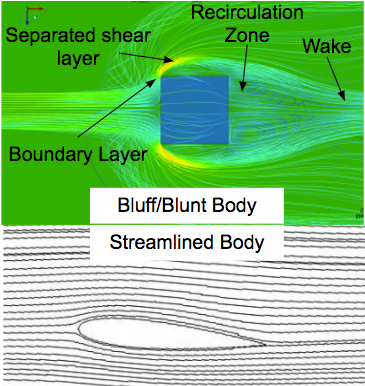
\includegraphics[width=0.45\textwidth]{Images/logan/bluntVSstreamline.png}
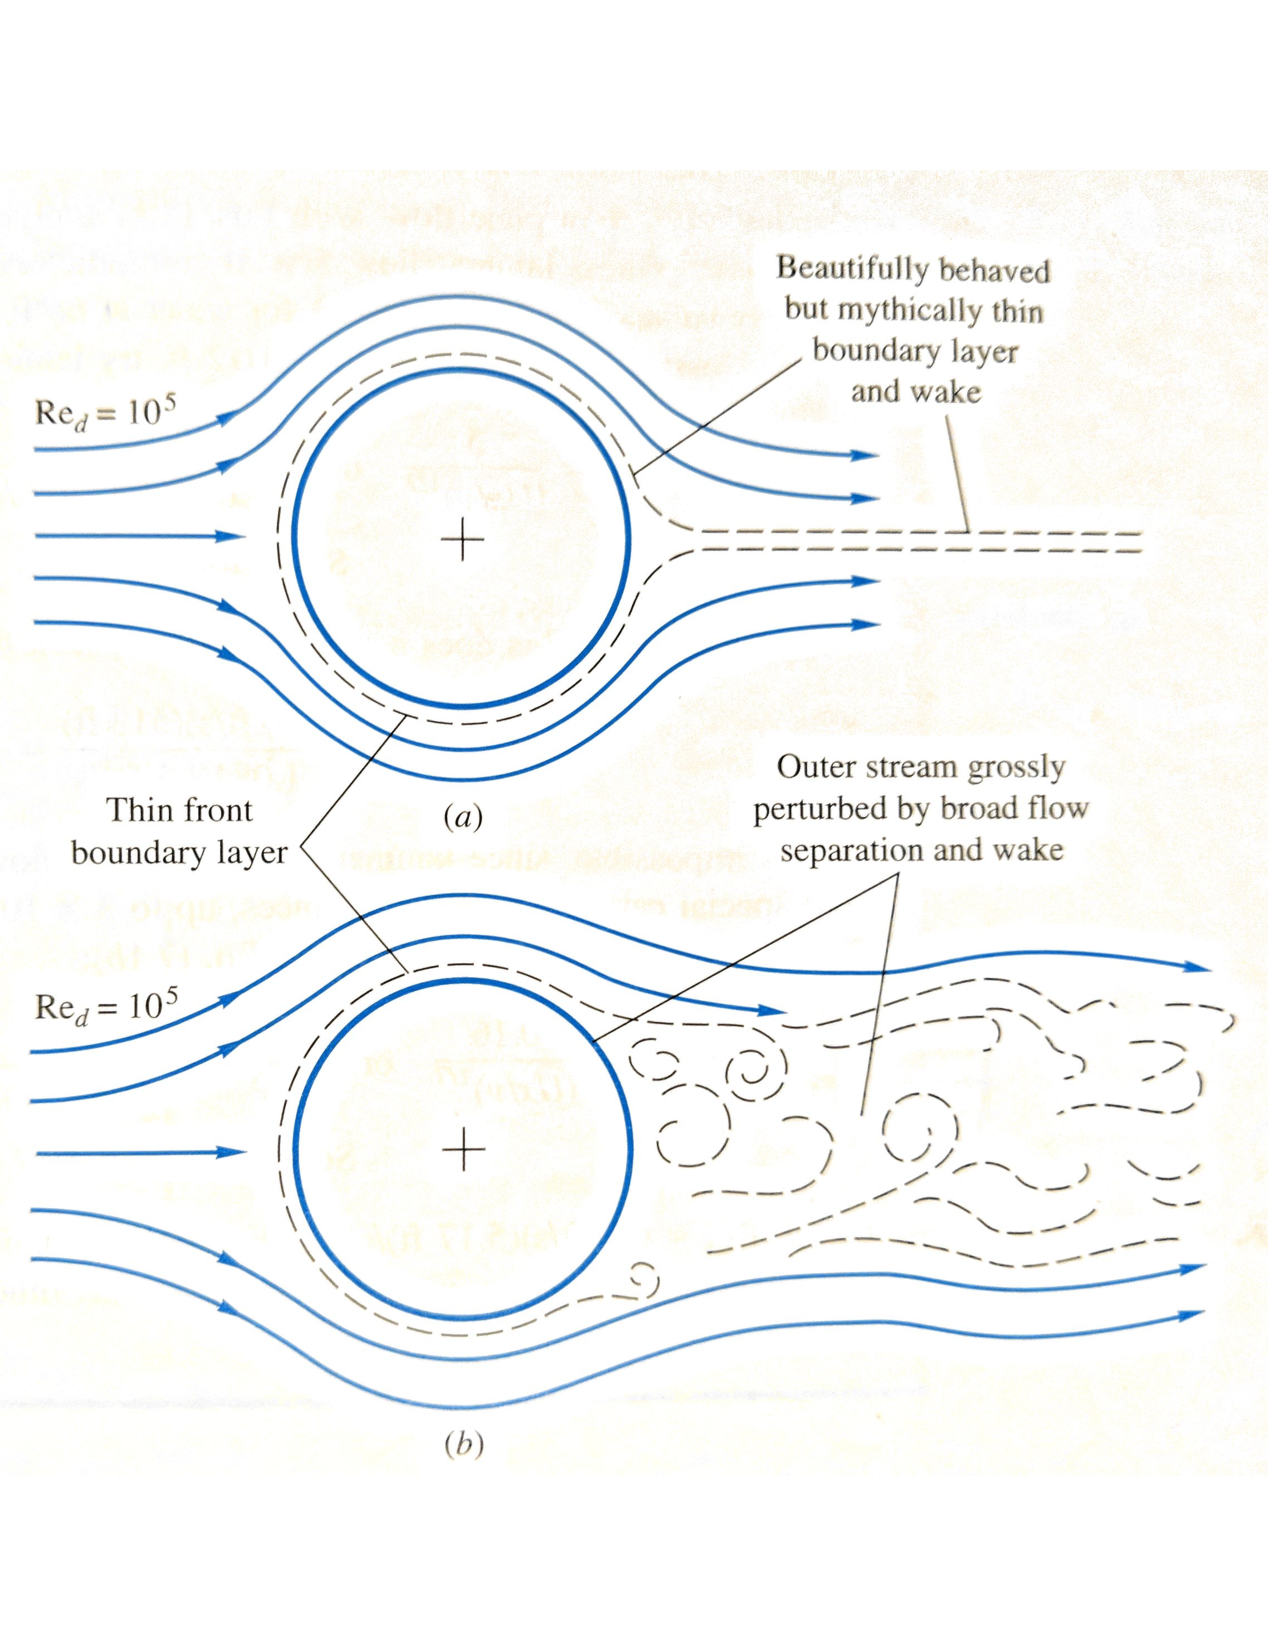
\includegraphics[width=0.49\textwidth]{Images/logan/white2011fluid_BluffBodyInviscidVSViscous.pdf}
\caption{ Demonstration of the flow differences between a bluff-body with massive separation \cite{richards2015modelling} and a streamlined body with primarily attached flow (left) and illustration of non-physical, inviscid flow over a bluff-body with no separation and realistic, viscous flow with massive separation (right) \cite{white2011fluid} }
\label{fig:bluffvsstreamlined}
\end{center}
\end{figure}
%%\vspace{-2em}

For the sake of terminology commonly found in the literature pertaining to bluff-bodies, it is also relevant to define the concept of base pressure \cite{tanner1998theories}. Because the flow over bluff-bodies is characterized by massive separation and a detached shear layer, it follows that there will be no pressure recovery along the surface of the body in the separated region. Thus, the surface pressure along the aft of a bluff-body remains at a nearly constant value, which is commonly described as a ``base pressure''.  This base pressure value is lower than that which would be found in an equivalent but non-physical ``inviscid'' flow, as is illustrated by Frank White in the right of Fig~\ref{fig:bluffvsstreamlined}, where attached flow would allow the pressure to rise again to stagnation values at the back of the sphere.  Base pressure is thus the primary contributor the the dominating pressure drag of the bluff-body. It is also important to note that bluff-body flows may be called ``base flows'' in reference to the base pressure.












%%%%%%%%%%%%%%%%%%%%%%%%%%%%%%%%%%%%%%%%%%%%%%%%%%%%%%%%%%%%
%REAL WORLD APPLICATIONS

Bluff-body flow is applicable to a plethora of real-world applications.  Massively separated wakes are characterized by complex, unsteady, and sometime unstable turbulent phenomena, which can lead to design concerns throughout the fields of engineering. A few examples of bluff-body flow in engineering applications include wall-mounted cubes representative of a high-rise buildings \cite{elkhoury2016assessment}, bridge spans \cite{yuan2017investigation} as modeled in Fig~\ref{fig:tacomanarrowswake}, ground vehicles \cite{mendonca2002towards} like the passenger sedan shown in Fig~\ref{fig:carwake}, atmospheric reentry vehicles \cite{ross2013comprehensive} like the Orion wind tunnel model in Fig~\ref{fig:orionwakeandejectionseat}, humans in ejection seats and parachutes, both demonstrated in Fig~\ref{fig:orionwakeandejectionseat}, aircraft protuberances such as landing-gear trucks, space launch vehicles, and flame holders \cite{tanaka2013bluff} in combustors (Fig~\ref{fig:flameholder}).

Bluff-bodies are common in civil engineering applications, where engineers might be concerned in predicting unsteady wind loading leading to structural resonance, which was a major design flaw for the Tacoma Narrows Bridge.  Fig~\ref{fig:tacomanarrowswake} demonstrates a model bridge span undergoing wake-induced vibration due to the vortex shedding caused by the gap in the center \cite{yuan2017investigation}.

%%% TACOMA NARROWS WAKE
%%\vspace{-2em}
% \begin{figure}[htb]
\begin{figure}[H]
\begin{center}
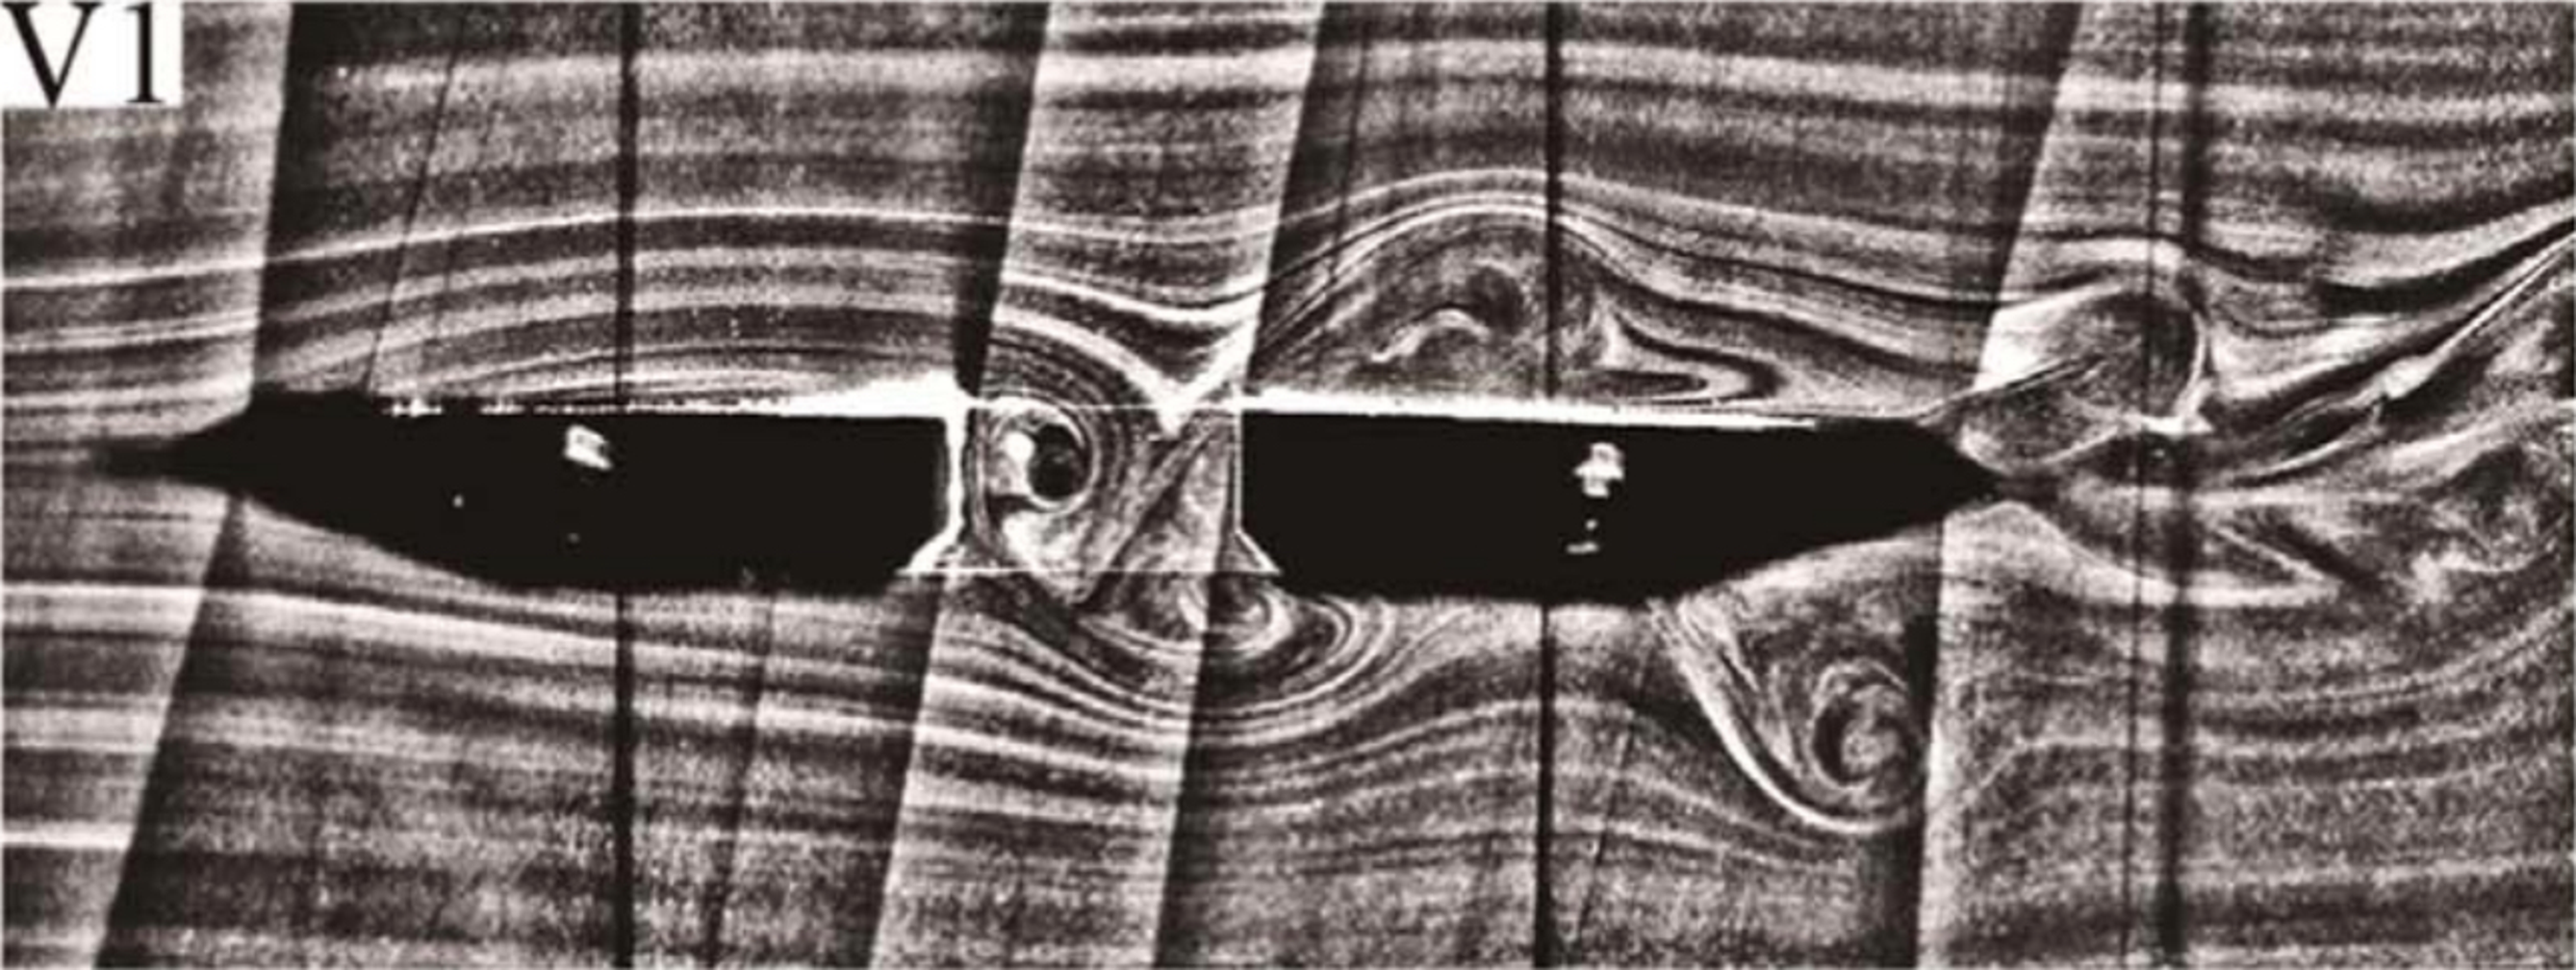
\includegraphics[width=0.7\textwidth]{Images/logan/yuan2017investigation_TacomaNarrowsWake.pdf}
\caption{ Instantaneous PIV flow field of bridge model similar to Tacoma Narrows bridge (Re=587) \cite{yuan2017investigation} }
\label{fig:tacomanarrowswake}
\end{center}
\end{figure}
%%\vspace{-2em}

Unsteady loading and buffeting can also be a potentially catastrophic bluff-body wake effect for mechanical and aerospace engineering applications.  The dynamic situation of a cockpit emergency egress system as depicted in Fig~\ref{fig:orionwakeandejectionseat} requires precise understanding of the unsteady forces on the ejection seat and human in order to mitigate any injuries the escaping pilot might experience.

Dynamic stability can also be adversely affected by bluff-body wake behavior.  The drogue parachute in Fig~\ref{fig:orionwakeandejectionseat} and the model Orion capsule in Fig~\ref{fig:orionwakeandejectionseat} are both situations where dynamic instability of the bluff-body could lead to potentially fatal situations for the humans involved.

%%% EJECTION SEAT and ORION WAKE
%%\vspace{-2em}
% \begin{figure}[htb]
\begin{figure}[H]
\begin{center}
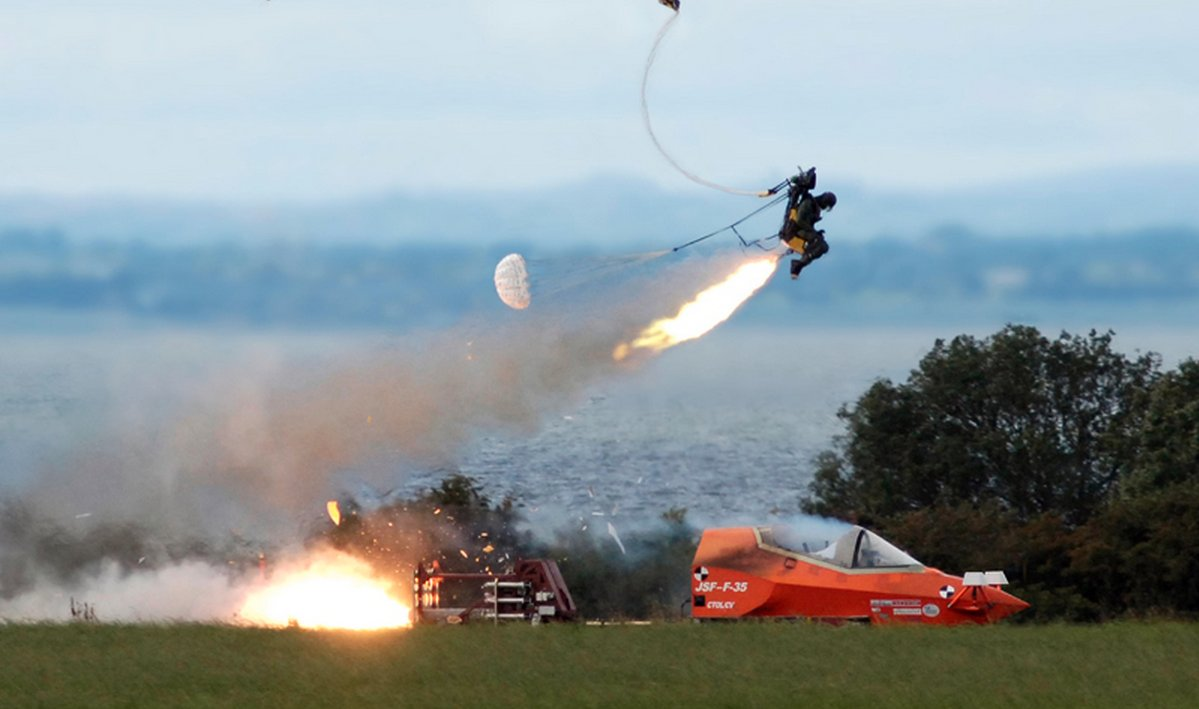
\includegraphics[width=0.48\textwidth]{Images/logan/martinbaker_EjectionSeat.jpg}
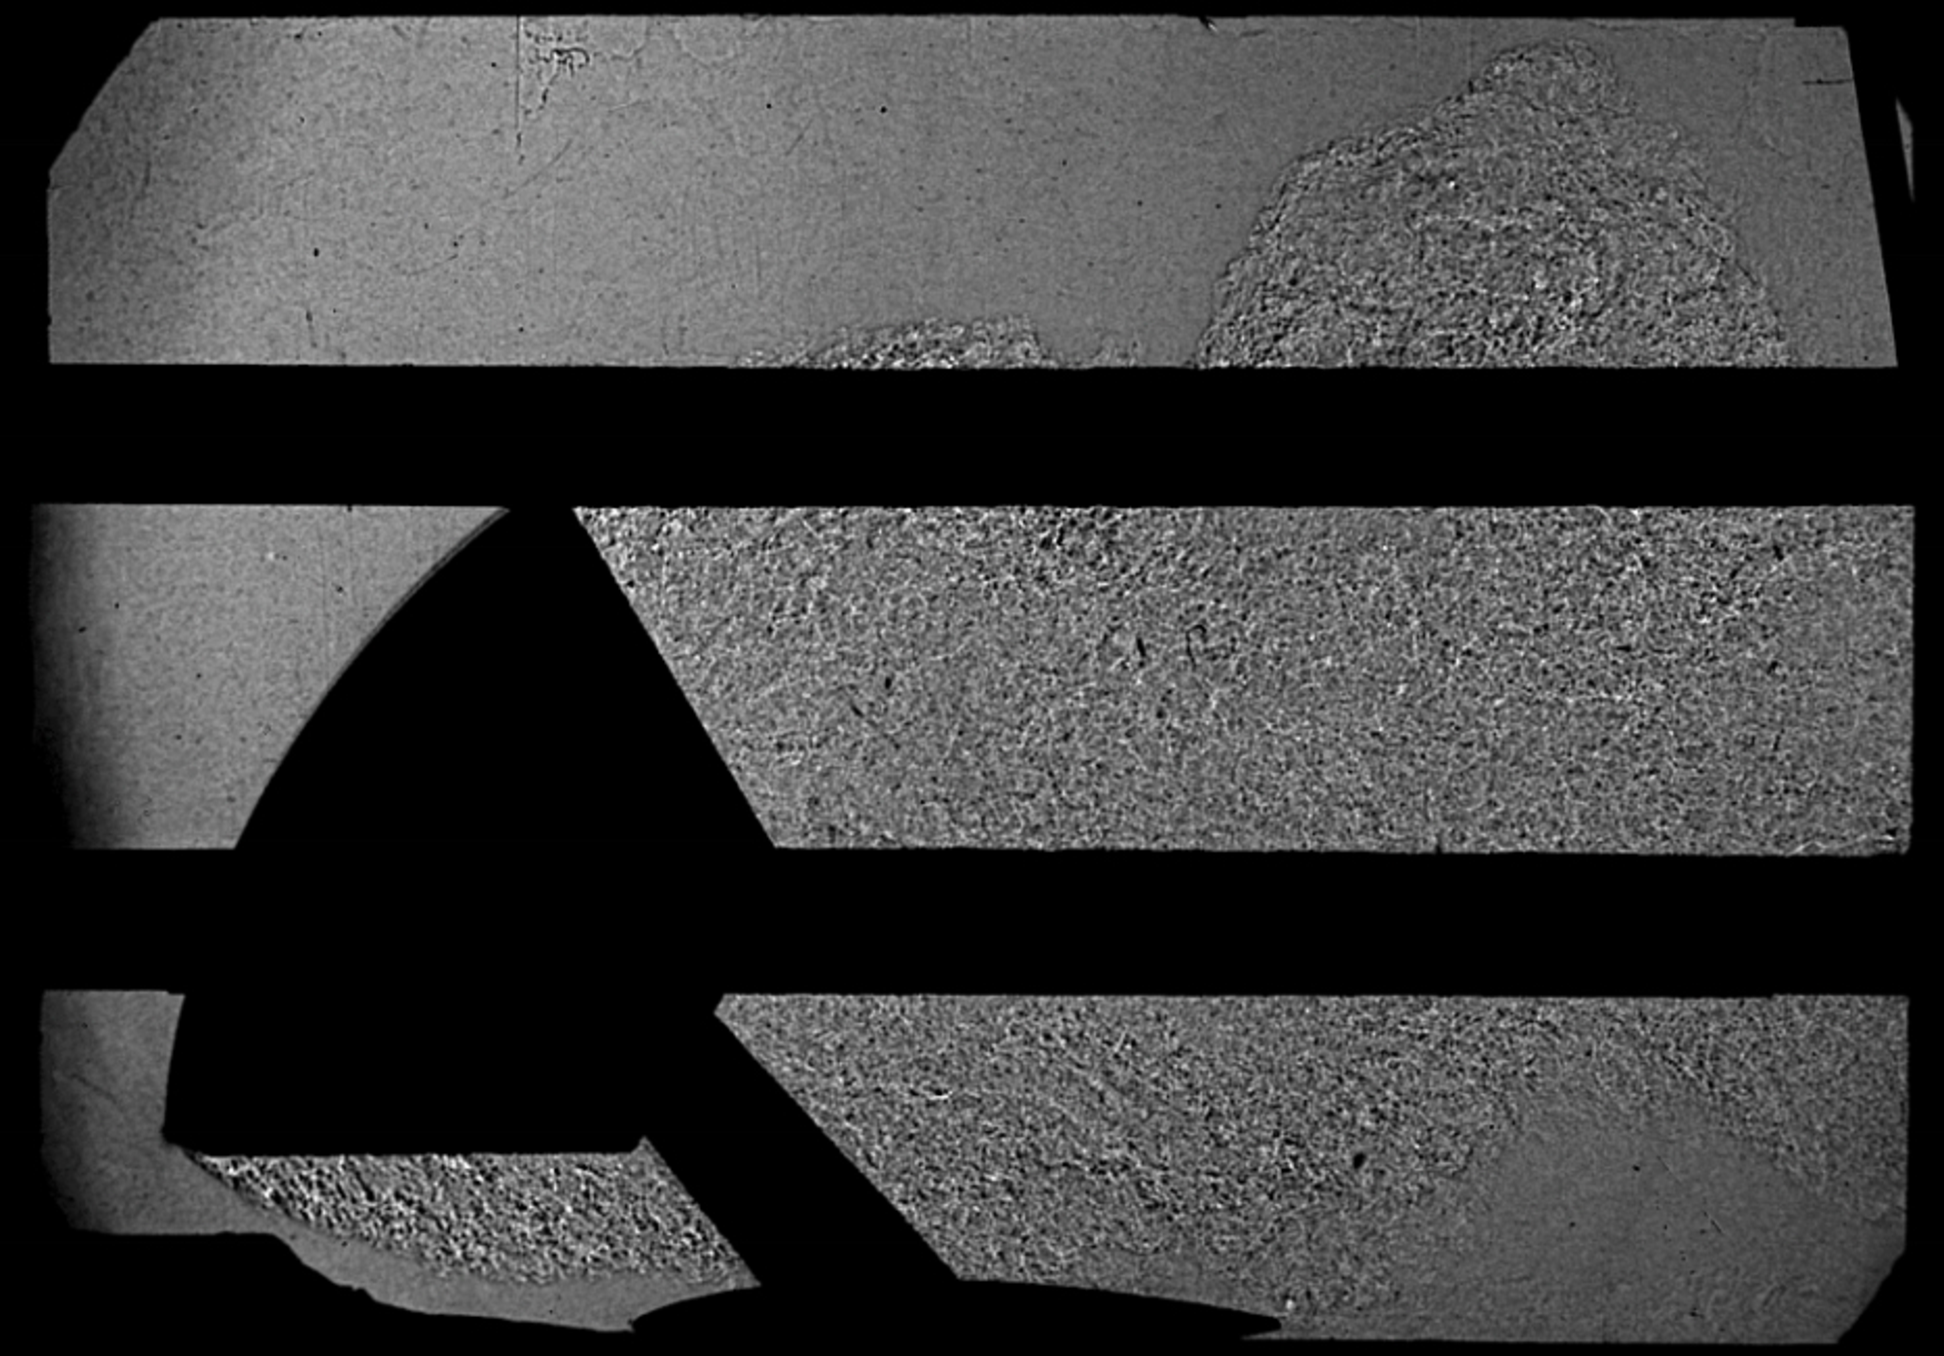
\includegraphics[width=0.41\textwidth]{Images/logan/ross2013comprehensive_CapsuleWakeShadowgraph.pdf}
\caption{ Left: Mk-16 ejection seat rocket sled test (Martin-Baker), Right: Shadowgraph wake of Orion capsule model ($M=0.3, \alpha=29.25^o, Re_D = 5.3\times10^6$) \cite{ross2013comprehensive}}
\label{fig:orionwakeandejectionseat}
\end{center}
\end{figure}
%%\vspace{-2em}



Acoustics can also be a design concern either due to unsteady loading as in the case of a launch vehicle or due to noise concerns or restrictions such as those for aircraft noise. Even passenger vehicles like the one shown in Fig~\ref{fig:carwake} can create a separated wake which can lead to acoustic disturbance of the passengers inside.

%%% CAR WAKE
%%\vspace{-2em}
% \begin{figure}[htb]
\begin{figure}[H]
\begin{center}
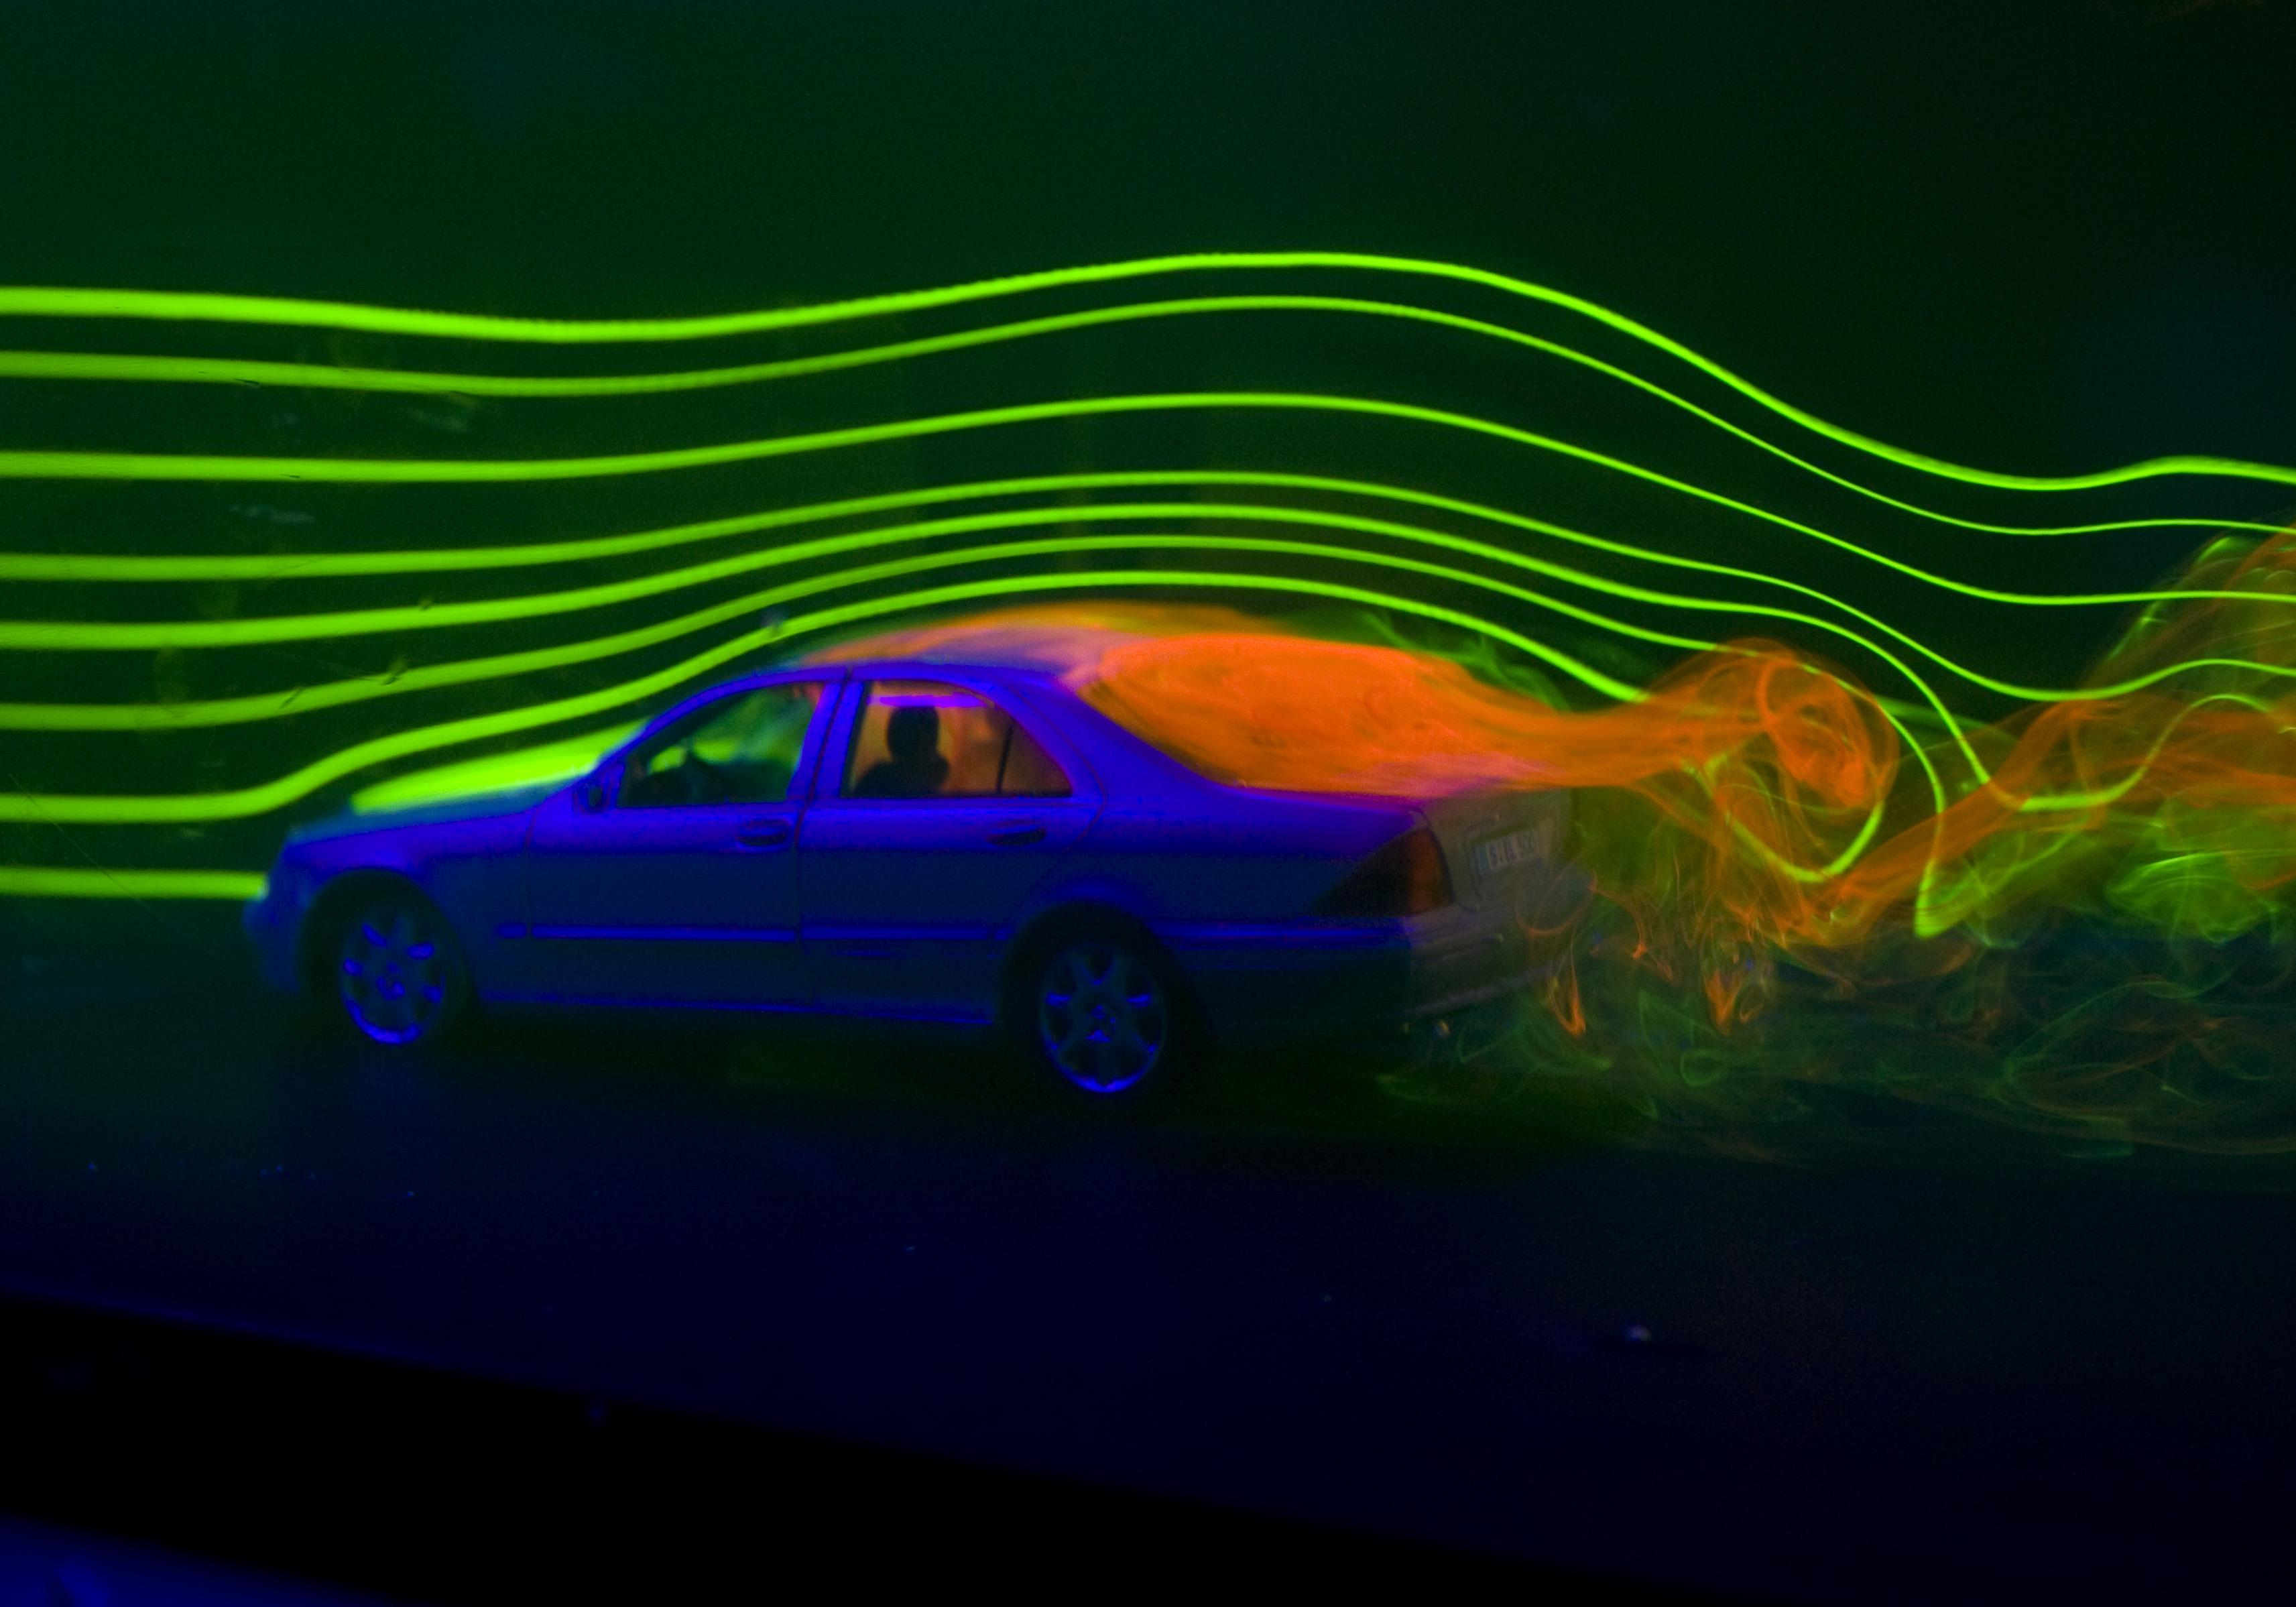
\includegraphics[width=0.5\textwidth]{Images/logan/james_CarWakePIV.jpg}
\caption{ Streamlines and separated flow over a car in a wind tunnel (NASA/Eric James) }
\label{fig:carwake}
\end{center}
\end{figure}
%%\vspace{-2em}

There are even applications of bluff-bodies outside the concepts of loading and acoustics. In industrial applications where a high-speed mixture must be ignited, it is necessary to both reduce the speed and mix the flow around an ignition source to allow a flame to stabilize. This effect can be created by placing a triangular bluff-body directly upstream of an ignitor such that its recirculation region entrains slower-moving mixture at the ignitor's location (Fig~\ref{fig:flameholder}) \cite{li2011large}.

%%% BLUFF BODY FLAME HOLDER
%%\vspace{-2em}
% \begin{figure}[htb]
\begin{figure}[H]
\begin{center}
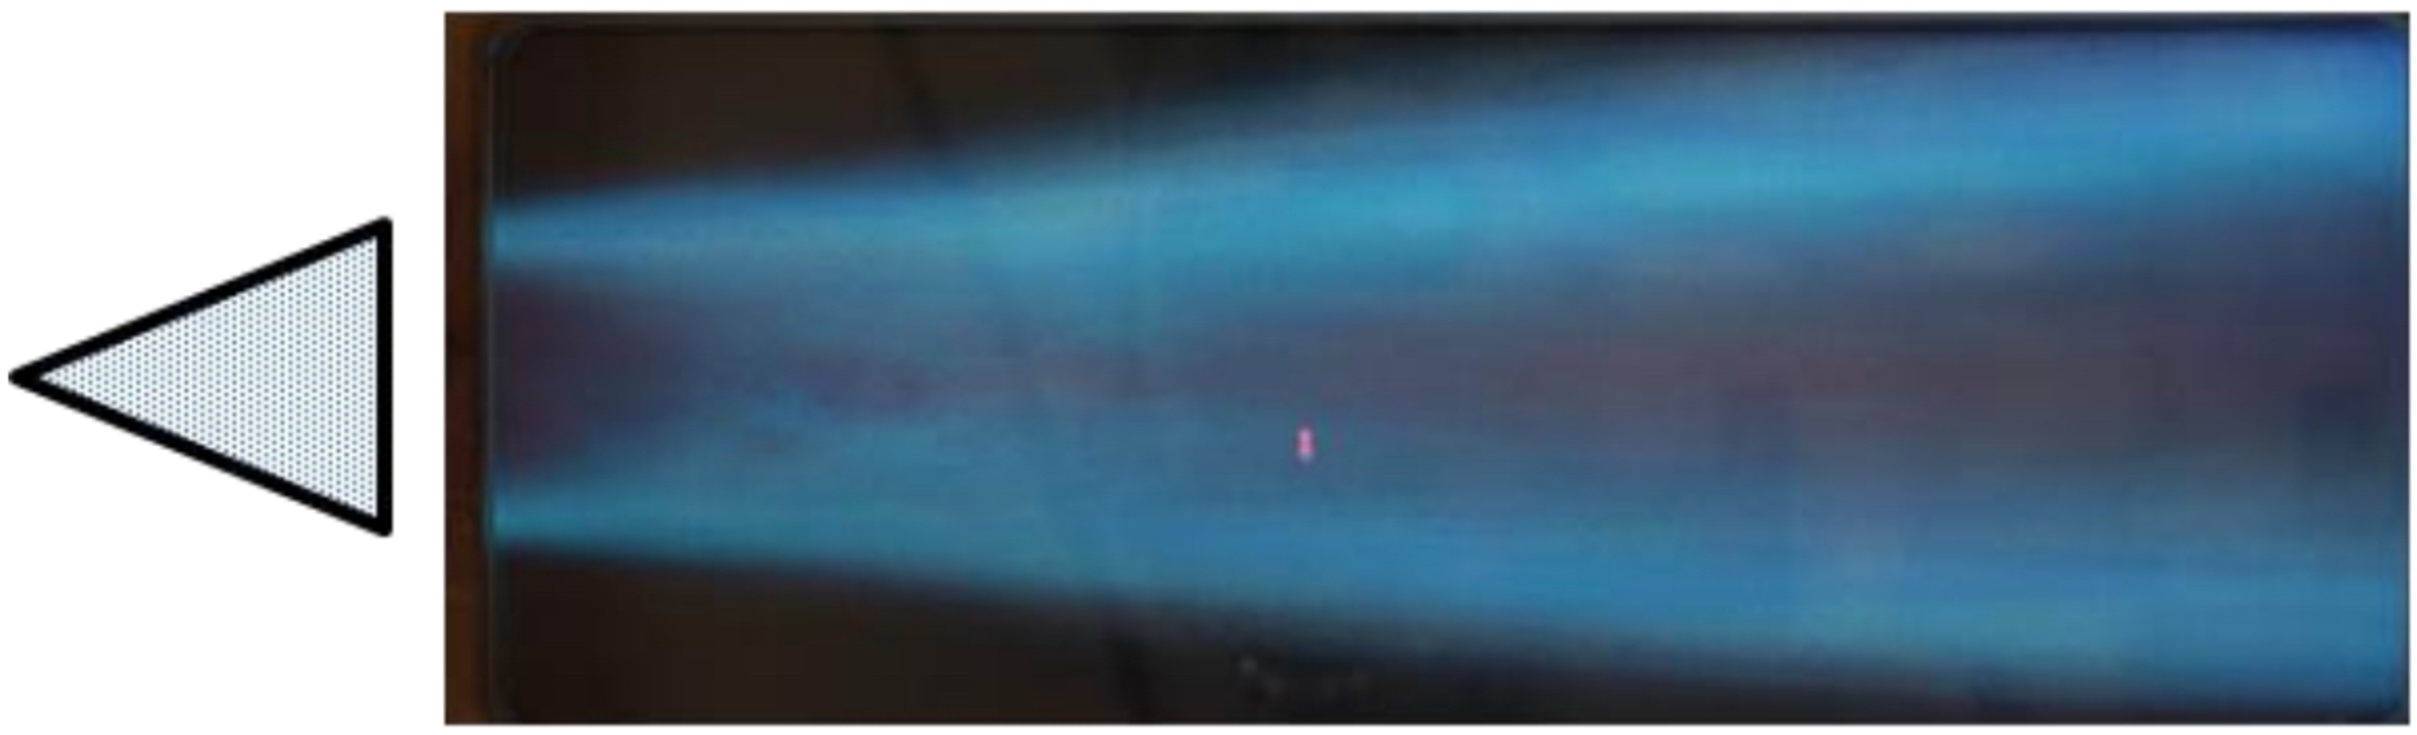
\includegraphics[width=0.7\textwidth]{Images/logan/tanaka2013bluff_FlameHolder.pdf}
\caption{ Image of a stabilized flame held in the wake of a bluff-body flame holder \cite{tanaka2013bluff} }
\label{fig:flameholder}
\end{center}
\end{figure}
%%\vspace{-2em}



The wakes of bluff-bodies are extremely complex, containing many scales of turbulent structures and can be highly unstable. These facts simultaneously impress upon the importance of understanding the effects of bluff-body flows for engineering applications and give rise to long-term difficulties in modeling and observing bluff-body flow. This review will attempt to connect the entire field of bluff-body fluid dynamics, archiving the fundamental concepts and historical approaches, assessing modern techniques of experimental and computational analysis, and discussing the challenges that remain.



% \emph{Big whorls have little whorls, which feed on their velocity, and little whorls have lesser whorls, and so on to viscosity (in the molecular sense).}
% Richardson (1922) \cite{richardson1922weather}





































%%%%%%%%%%%%%%%%%%%%%%%%%%%%%%%%%%%%%%%%%%%%%%%%%%%%%%%%%%%%%%%%%%%%%%%%
\section{Flow around a bluff body and transition}
%%%%%%%%%%%%%%%%%%%%%%%%%%%%%%%%%%%%%%%%%%%%%%%%%%%%%%%%%%%%%%%%%%%%%%%%

Despite the differences between the shapes of bluff bodies, the disturbed flow around them have some similarities. Bluff bodies generate an alteration in the surrounding velocity, and flow around them can be bigger than, equal to or smaller than the free stream velocity. When describing the flow around a cylinder, ideally  the description would be general for bluff bodies, independently of their shape. The present state of knowledge is still not capable of doing this, and so the description will depend on the shape of the body. In this section we are going to describe one of the most common and studied shapes of bluff bodies: circular cylinders. Figure \ref{fig:RegionsFlow} shows a scheme of the flow around a circular cylinder with the different regions of disturbed flow. The different regions are:

\begin{enumerate}[label=(\roman*)]
\item A thin region of retarded flow.
\item Two boundary layers attached to the surface.
\item Two regions adjacent to the cylinder with accelerated flow.
\item One region downstream the cylinder of separated flow, usually called wake.
\end{enumerate}

\begin{figure}[H]
\begin{center}
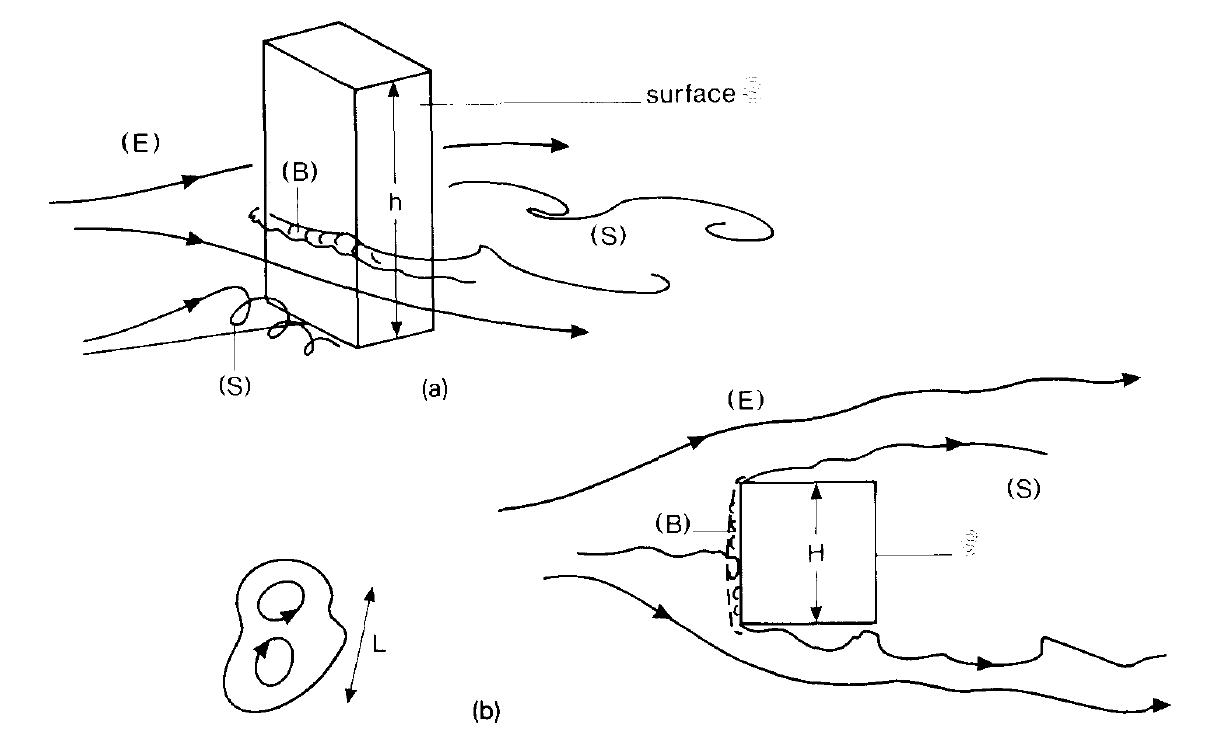
\includegraphics[width=0.7\textwidth]{Images/federico/Figure01}
\caption{ Regions of disturbed flow around a circular cylinder. Extracted from \cite{Zdravkovich1997} }
\label{fig:RegionsFlow}
\end{center}
\end{figure}

Although flow around circular cylinders usually present all these regions, their shape, size and flow structures depends on various parameters, but especially on the Reynolds number ($Re$). The Reynolds number is the parameter that usually describes the transition from laminar to turbulent flow. In the case of circular cylinders, transition can begin in different regions of the disturbed flow. The first transition appears in the wake, where turbulence is developed in the wake but the shear layer around the near-wake remain laminar. The second transition appears in the shear layer close to the near-wake and, as $Re$ increases, the transition gets closer to the boundary layer, leading to the third transition to turbulence, transition in the boundary layer. Transition in boundary layer was one of the most studied transitions in this type of flows, because it causes a sudden decrease in the drag force, usually denominated 'drag crisis'.

The Reynolds number is considered the governing parameter around a circular cylinder only for disturbance-free flows. In real flows, other variables may affect the flow around bluff bodies. These variables are usually called influencing parameters. When the effect of these parameters is important, they may become into governing parameters. Common influencing parameters found in real flows are free stream turbulence, surface roughness, wall proximity, non-uniform free stream flow, oscillatory free stream flow, between others. All these parameters will modify the beginning and the end of the different flows regimes around bluff bodies, and they even cause the disappearance of some of the regimes. A very known example is how a rough sphere generate transition to turbulent boundary layers for lower $Re$ than a smooth sphere.

In the following section we are going to describe the different flow regimes around a circular cylinder as a function of $Re$ for a free-disturbance flow. The regimes will be divided into five regimes, and those regimes into sub-regimes

\begin{enumerate}[label=(\roman*)]
\item Laminar regime (L)
\item Transition in wake regime regime (TrW)
\item Transition in shear-layer regime (TrSL)
\item Transition in boundary-layer regime (TrBL)
\item Fully turbulent Regime (T)
\end{enumerate}

%%%%%%%%%%%%%%%%%%%%%%%%%%%%%%%%%%%%%%%%%%%%%%%%%%%%%%%%%%%%%%%%%%%%%%%%
\subsection{Laminar regime (L)}

The laminar state can be divided into three different flow regimes:

\begin{enumerate}[label=(\roman*)]
\item L1: Creeping flow regime  $0<Re<4-5$
\item L2: Steady separation regime $4-5<Re<30-48$
\item L3: Periodic laminar regime $30-48<Re<180-200$
\end{enumerate}

Creeping flow (L1) only occurs for very low $Re$ and its dominated by viscous forces. In this regime there is not visible separation, and the flow is similar to the one predicted by the potential theory.  When  $Re$ increases the effect of the viscous forces decrease, until at a $Re$ of 4 or 5 the flow separates. This separation is cause due to a favorable pressure gradient in the surface of the cylinder. The steady separation regime (L2) is characterized for two shear layers that form a steady, closed and symmetric wake. Behind the cylinder there is a weak recirculating flow that form two symmetric eddies.

This wake becomes unstable for $Re > 30-48$, starting the denominated periodic laminar regime (L3). In this regime any disturbance generates an oscillation that is amplified, causing a wavy trail after the cylinder. The amplitude of the oscillation increase with $Re$ until the two shear layers begin to interact with each other, forming eddies that are shed downstream, forming the well known Von-Karman eddy street.


\begin{figure}[H]
\begin{center}
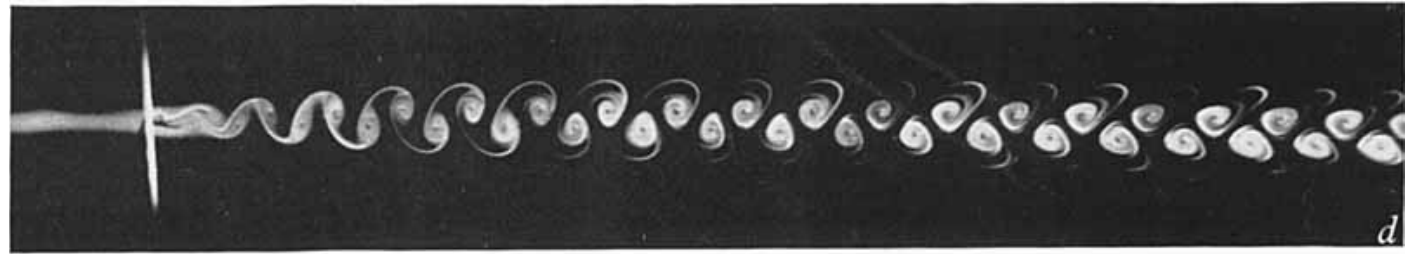
\includegraphics[width=1\textwidth]{Images/federico/Figure02}
\caption{Kárman-Bénard eddy street at \textbf{\textit{Re = 100}}. Extracted from \cite{Zdravkovich1968} }
\label{fig:Laminar}
\end{center}
\end{figure}

A picture of a fully developed Von-Karman eddy street is shown in Figure \ref{fig:Laminar}. It was generated by Zdravkovich (1968) \citep{Zdravkovich1968} in a wind tunnel using liquid kerosene in the form of a fog of fine droplets. We can see that the eddies initiated at the end of the closed near wake and that after some length downstream the cylinder the patterns become 'frozen', meaning that they practically do not change their shape. This effect appears because these 'frozen' eddies are present where the wake have already disappeared, and they are only the remaining shapes of smoke that are advected downstream by a uniform flow, without affecting their structure. Another feature that can be noticed in Figure \ref{fig:Laminar} is that the widening of the wake occurs due to the entrainment of the external fluid.

The periodic laminar regime is truly two dimensional for $40<Re<80$. For  $80<Re<100$ the wake become sensitive to perturbations and may become three dimensional and it is always three dimensional for  $100<Re<160$ \cite{Phillips1956}. This three dimensionality of the flow may lead to transition for higher $Re$.

\Huge{\textcolor{red}{STROUHAL NUMBER}}

\normalsize



%%%%%%%%%%%%%%%%%%%%%%%%%%%%%%%%%%%%%%%%%%%%%%%%%%%%%%%%%%%%%%%%%%%%%%%%
\subsection{Transition in wake (TrW)}

Only in rare cases a flow instability does not lead to transition to turbulence. The flow in the wake of a circular cylinder will eventually become turbulent if $Re$ is increased. The transition in wake may be divided into two regimes:

\begin{enumerate}[label=(\roman*)]
\item TrW1: Lower transition regime. $180-200<Re<220-250$
\item TrW2: Upper transition regime. $220-250<Re<350-400$
\end{enumerate}

In the lower transition regime (TrW1) the eddies are formed laminar but become turbulent downstream after they have been shed (Figure \ref{fig:TrW1}). This transition will spread upstream with increasing $Re$. In the upper transition regime (TrW2) the eddies are formed laminar but become turbulent before they are shed (Figure \ref{fig:TrW2}). The shear layers remain laminar, even for the TrW2 regime.

\begin{figure}[H]
\begin{center}
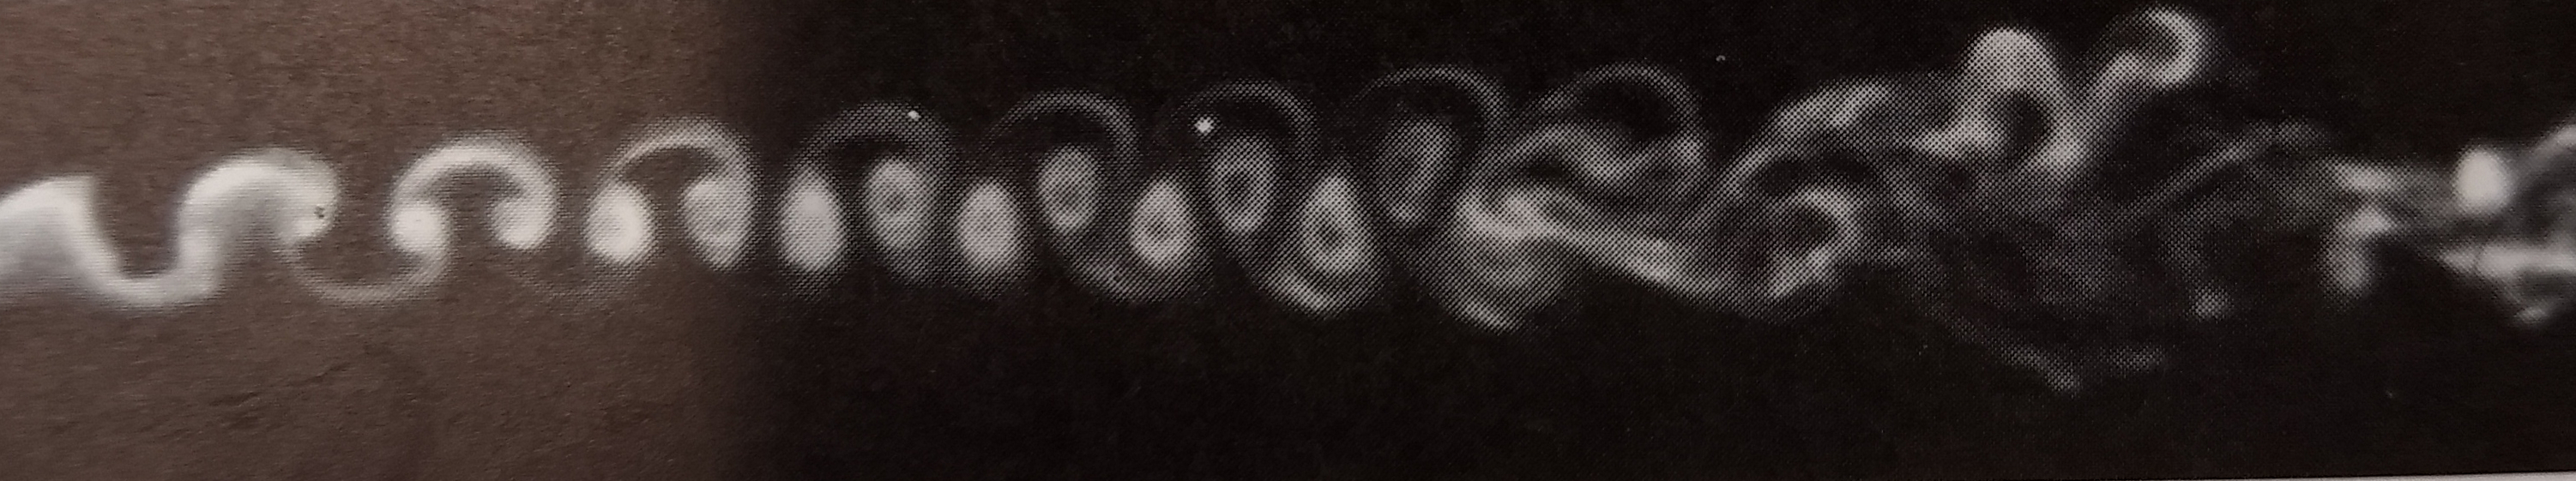
\includegraphics[width=1\textwidth]{Images/federico/Figure03}
\caption{Transition in wake 1 at \textbf{\textit{Re = 190}}. Extracted from \cite{Zdravkovich1968} }
\label{fig:TrW1}
\end{center}
\end{figure}

When $Re>150$ a peculiar type of distortion of the eddy filaments next to the cylinder appear. Gerrard (1978) \cite{Gerrard1978} called them 'fingers' because these distortions pointed towards the cylinder. These 'fingers' do not produce turbulent eddies, but they do produce a highly three dimensional flow which is still laminar. At some point downstream these structures desintegrate themselves becoming turbulent.


\begin{figure}[H]
\begin{center}
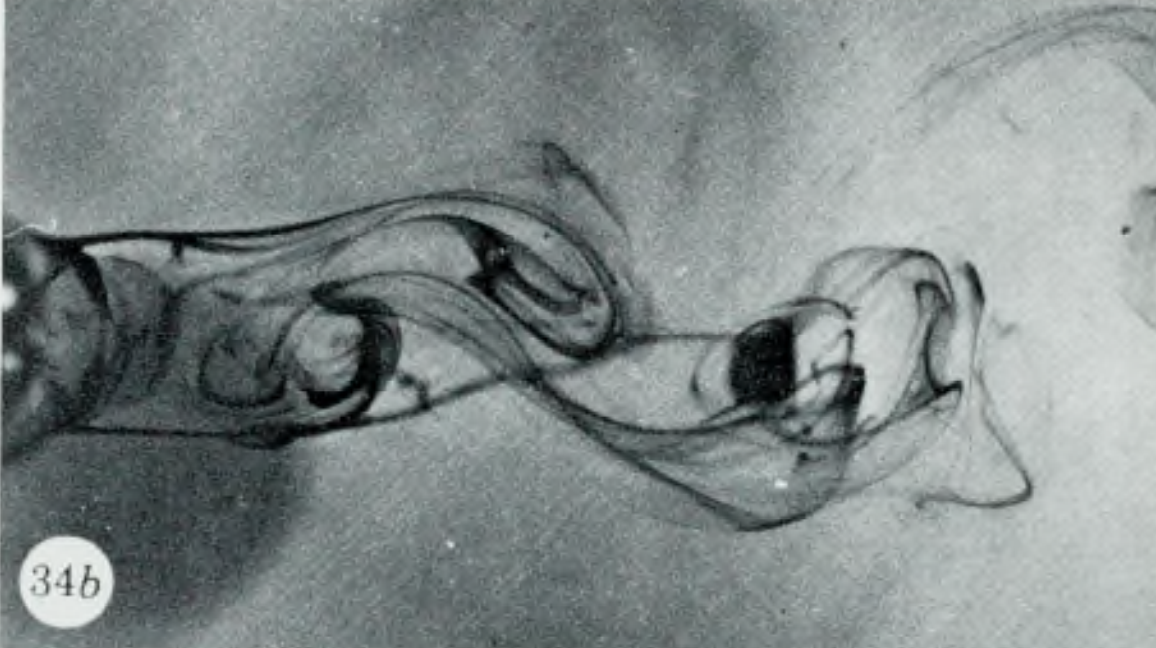
\includegraphics[width=0.5\textwidth]{Images/federico/Figure04}
\caption{Transition in wake 2 at \textbf{\textit{Re = 344}}. Extracted from \cite{Gerrard1978} }
\label{fig:TrW2}
\end{center}
\end{figure}

%%%%%%%%%%%%%%%%%%%%%%%%%%%%%%%%%%%%%%%%%%%%%%%%%%%%%%%%%%%%%%%%%%%%%%%%
\subsection{Transition in shear layers (TrSL)}

In the TrW regime, the shear layer surrounding the near-wake eddies remain laminar. The transition to turbulence in shear layer can be divided into three regimes:

\begin{enumerate}[label=(\roman*)]
\item TrSL1: Development of transition waves. $350-400<Re<1k-2k$
\item TrSL2: Formation of transition eddies. $1k-2k<Re<20k-40k$
\item TrSL3: Burst to turbulence. $20k-40k<Re<100k-200k$
\end{enumerate}

In the TrSL1 regime transition waves appear in the free surface. Similar waves to those found in boundary layer (Tollmien-Schlichting waves) were observed in the transition of the shear layer behind a bluff body (Figure \ref{fig:TrSL}). The Gerrard-Bloor transition waves were found in the shear layer behind cylinders beyond $Re=500$ \cite{Gerrard1978}. These waves are characterized for being symmetric and parallel to the wake axis, indicating that they are two dimensional. The wake becomes irregular downstream the wake, after the transition to turbulence.

\begin{figure}[H]
\begin{center}
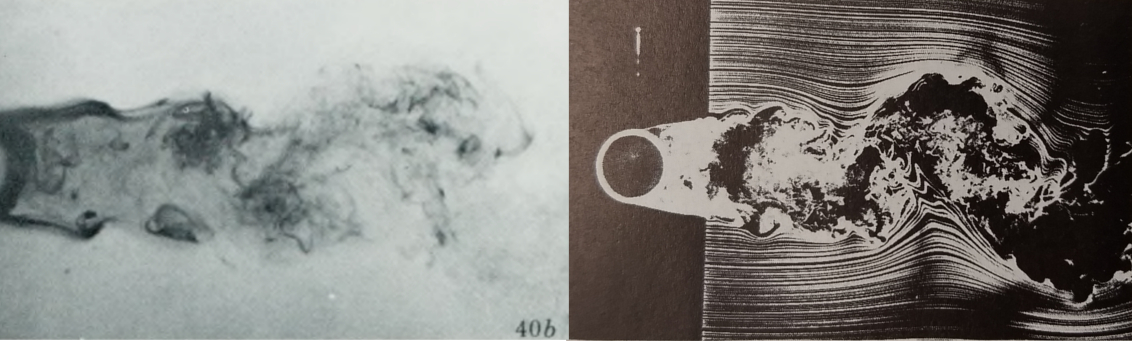
\includegraphics[width=1\textwidth]{Images/federico/Figure05}
\caption{Transition in free shear layer. Left: \textbf{\textit{Re = 1083}}. Extracted from \cite{Gerrard1978}. Right: \textbf{\textit{Re = 8000}}. Extracted from \cite{Zdravkovich1997}}
\label{fig:TrSL}
\end{center}
\end{figure}

In the TrSL2 regime, a chain of transition eddies are formed along the shear layer, incorporating free stream flow to the wake (Figure \ref{fig:TrSL}). They eventually roll up forming a large turbulent eddy.  As $Re$ increases the formation of eddies  gets closer to the cylinder, until the shear layer becomes fully turbulent, marking the beginning of TrSL3 regime. Once this regime starts, the formation of eddies do not change its position (e.g. do not get closer to the cylinder) and the transition is reduced to a spot of sudden burst into turbulence.

%%%%%%%%%%%%%%%%%%%%%%%%%%%%%%%%%%%%%%%%%%%%%%%%%%%%%%%%%%%%%%%%%%%%%%%%
\subsection{Transition in boundary layer (TrBL)}

The advance of transition to turbulence to the separated boundary layer in the TrSL regime is limited because  the separated shear layers are squeezed beyond the separation by the accelerated free stream. This effect is reduced with increasing $Re$, allowing the  beginning of the transition in boundary layer regime (TrBL). The turbulent boundary layer reattaches to the surface and the separation point gradually moves downstream. In order to be able to create a physical model that represent this regime, cylinders should be large enough and so huge wind tunnels are necessary to place them. Because of this reason many of the experiments performed to study this regime are affected by many influencing parameters. The TrBL state can be divided in five regimes:

\begin{enumerate}[label=(\roman*)]
\item TrBL0: Precritical regime. $100k-200k<Re<300k-340k$
\item TrBL1: One-bubble regime. $300k-340k<Re<380k-400k$
\item TrBL2: Two-buble regime. $380k-400k<Re<0.5M-1M$
\item TrBL3: Supercritical regime. $0.5M-1M<Re<3.4M-6M$
\item TrBL4: Post-critical regime. $3.4M-6M<Re<unkown$
\end{enumerate}

The precritical regime (TrBL0) in characterized by a gradual displacement of the separation downstream with rising $Re$. This regime end abruptly with a discontinuous fall in the drag coefficient and a jump in the frequency of the eddy shedding. The one-bubble regime in characterized for an asymmetric pressure distribution on the sides of the cylinder. This effect appears because only on one side of the cylinder the boundary layer reattached to the surface. This effect also leads to an asymmetric near wake (Figure \ref{fig:TrBL}). The formation of the bubble may appear in any of the two sides, but once it appear, it does not change side \citep{Zdravkovich1997}. The reattachment of the boundary layer lead to a reduction in the wake's width and an increase in the shedding frequency. 


\begin{figure}[H]
\begin{center}
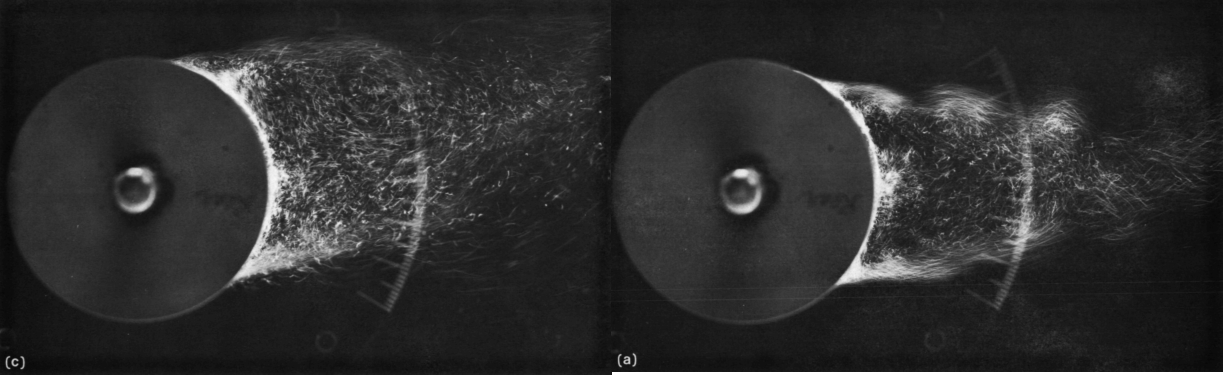
\includegraphics[width=1\textwidth]{Images/federico/Figure06}
\caption{Transition in boundary layer. Left: One-bubble regime \textbf{\textit{Re = 338k}}. Right: Two-bubble regime \textbf{\textit{Re = 374k}}. Extracted from \cite{Almosnino1984}}
\label{fig:TrBL}
\end{center}
\end{figure}


The one-bubble regime is only stable for a low range of $Re$. When $Re$ increases this regime ends abruptly as the two-bubble regime starts (TrBL2). The two-bubble regime is characterized for a second abrupt decrease in the drag coefficient, an increase in the base pressure, and a reattachment of the second boundary layer. TrBL1 and TrBL2  regimes are very sensitive to perturbations and can be eliminated with a rough surface.

If $Re$ increases the primary laminar separation becomes transitional, leading to a disruption and fragmentation in the separation bubbles along the cylinder. This fragmentation prevents eddy shedding, which is the most notable characteristic of the supercritical regime (TrBL3).As $Re$ increases the beginning of the turbulent boundary layers move upstream. The post-critical regime (TrBL4) is defined when they start somewhere between the separation and the stagnation points. As $Re$ increases the transition region advance downstream asymptotically in the direction of the stagnation point and this is why the limit of the TrBL4 is hard to define.   




%%%%%%%%%%%%%%%%%%%%%%%%%%%%%%%%%%%%%%%%%%%%%%%%%%%%%%%%%%%%%%%%%%%%%%%%
\subsection{Fully turbulent regime}

The fully turbulent regime is reached when all the disturbed flow regions become turbulent. It is unexpected to have any other type of transition when this state is reached, but this hypothesis in extremely difficult to test experimentally. This state would be achieved with extremely high $Re$, and this can be done by increasing the size of the cylinder or the velocity. The former is limited by the size of the wind tunnels while the former by effect of compressibility in air, and cavitation in water. Some examples of this type of flows can be found in geophysical flows of high scale, like ocean currents or atmospheric wind past islands (Figure \ref{fig:T}).

\begin{figure}[H]
\begin{center}
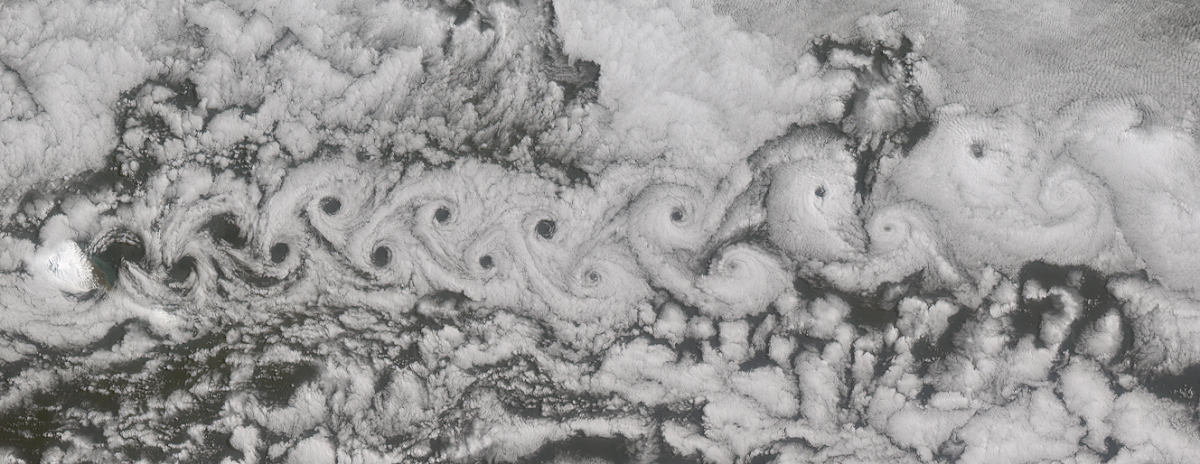
\includegraphics[width=1\textwidth]{Images/federico/Figure07}
\caption{Flow around a volcanic island. Retrieved from  \url{https://karlgaff.wordpress.com/karman-vortex-streets/}}
\label{fig:T}
\end{center}
\end{figure}


%%%%%%%%%%%%%%%%%%%%%%%%%%%%%%%%%%%%%%%%%%%%%%%%%%%%%%%%%%%%%%%%%%%%%%%%
\section{Free stream turbulence and non-uniform free stream}
%%%%%%%%%%%%%%%%%%%%%%%%%%%%%%%%%%%%%%%%%%%%%%%%%%%%%%%%%%%%%%%%%%%%%%%%

In the previous section, flow around a cylinder was analyzed for a free-disturbance flow. One of the parameters that affects flow around bluff bodies is free stream turbulence. Most flows in engineering applications are turbulent, and approaching turbulence interacts with flow structures past bluff bodies. One of the most classical examples of the influence of the free stream turbulence is the the reduction in the drag coefficient in cylinder and spheres \cite{Nakamura1988}. On the other hand, turbulence can increase the drag coefficient in square plates with its flat plate normal to the flow. 

In general, assuming a uniform and isotropic turbulence, the effect of free stream turbulence can be characterized by two parameters, turbulence intensity ($u'/U$) and turbulence lengthscale ($L_t$). Usually the lengthscale is used in its non-dimensional form, dividing it by the length of the bluff body ($L_t/h$).     

Free stream turbulence has an important effect the three types of transition to turbulence (TrW, TrSL, TrBL). Most experiments are made in wind tunnels with low-turbulence intensity, so the parameters obtained in these experiments cannot be extrapolated for real flows. Initiation of transition is particularly sensible to adverse pressure gradient, and fluctuating pressure due to turbulence imposes this gradient generating transition for lower $Re$ than those that generate transition in smooth flows.  

The interaction between free stream turbulence and flow structures is extremely complicated, and many research has been done to address this problem. In some cases the interaction is really important, like in the cases previously mentioned, and in some cases, the effect is almost negligible. An example of the latter is the interaction between free stream turbulence and eddies for TrW1 and TrW2 regime. In TrW1 regime, the effect of turbulence is only relevant when the velocity fluctuations are of the order of the intensity of the free stream turbulence \citep{Zdravkovich1997}. In the TrW2 regime, the transition to turbulence is almost insensitive to the free stream turbulence due to a stable laminar shear layer surrounding it.

The effect of free stream turbulence depends also on the shape of the bluff body. Nakamura \cite{nakamura1993bluffbody} tested the effect of turbulence intensity and turbulence lengthscale on the base pressure for a 3D square rod, a 2D rectangular cylinder and a 2D flat plate.  

\begin{figure}[H]
\begin{center}
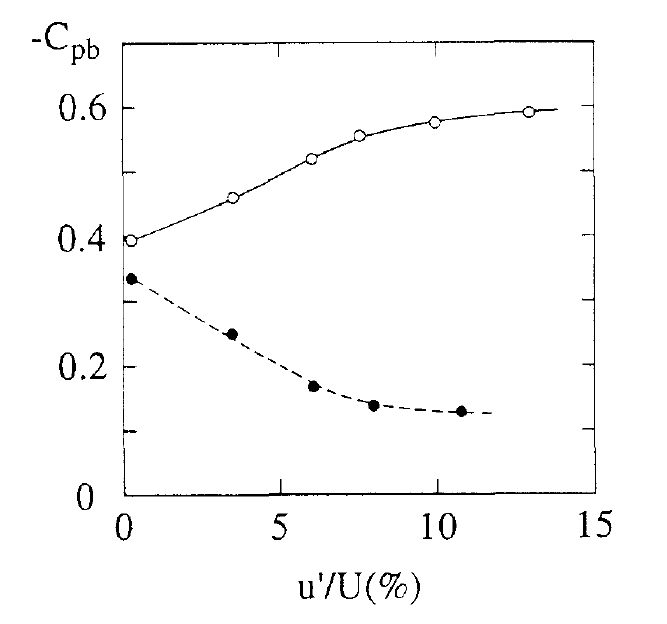
\includegraphics[width=0.4\textwidth]{Images/federico/Figure09}
\caption{Flow around a volcanic island. Retrieved from  \url{https://karlgaff.wordpress.com/karman-vortex-streets/}}
\label{fig:T}
\end{center}
\end{figure}


\begin{figure}[H]
\begin{center}
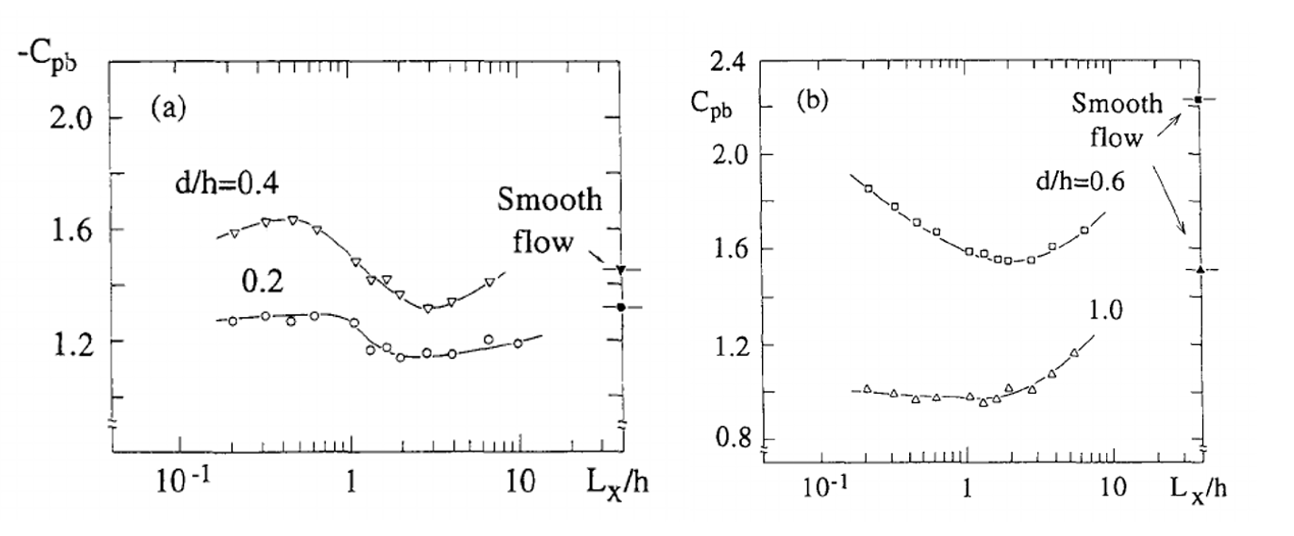
\includegraphics[width=0.8\textwidth]{Images/federico/Figure08}
\caption{Flow around a volcanic island. Retrieved from  \url{https://karlgaff.wordpress.com/karman-vortex-streets/}}
\label{fig:T}
\end{center}
\end{figure}



%%%%%%%%%%%%%%%%%%%%%%%%%%%%%%%%%%%%%%%%%%%%%%%%%%%%%%%%%%%%%%%%%%%%%%%%
\section{Experimental Methods And Results} \label{sec:experimentalmethods}
%%%%%%%%%%%%%%%%%%%%%%%%%%%%%%%%%%%%%%%%%%%%%%%%%%%%%%%%%%%%%%%%%%%%%%%%

\textcolor{red}{\emph{FZ}}

\begin{itemize}
    \item Historical Study
    \item Experimental techniques
    \begin{itemize}
        \item ballistic range?
    \end{itemize}
    \item Applications
    \begin{itemize}
        \item Simple cases: cylinder/sphere
        \begin{itemize}
            \item Drag vs Re?
            \item Wake velocity profiles?
            \item Wake structure?
        \end{itemize}
        \item Sharp vs bluff: sphere vs cube
        \item Complex cases: capsule/building
    \end{itemize}
\end{itemize}








%%%%%%%%%%%%%%%%%%%%%%%%%%%%%%%%%%%%%%%%%%%%%%%%%%%%%%%%%%%%%%%%%%%%%%%%
\subsection{Current State of Experimental Methods for Bluff-Body Flows} \label{subsec:currentstateexperimental}
































\clearpage

%%%%%%%%%%%%%%%%%%%%%%%%%%%%%%%%%%%%%%%%%%%%%%%%%%%%%%%%%%%%%%%%%%%%%%%%
\section{Computational Methods and Results} \label{sec:computationalmethods}
%%%%%%%%%%%%%%%%%%%%%%%%%%%%%%%%%%%%%%%%%%%%%%%%%%%%%%%%%%%%%%%%%%%%%%%%

Due to the highly complex nature of bluff-body wake separation and behavior, the primary realistic method of simulation for these flows is discrete solution of the Navier-Stokes equations (Eqn~\ref{eqn:navierstokes}) or Computational Fluid Dynamics (CFD). Analytic, inviscid formulations such as potential flow methods yield the non-physical results depicted in the top image of Fig~\ref{fig:bluffvsstreamlined}, where there is no separation or corresponding base pressure, making this fictional flow a non-bluff-body. The same deficiencies apply to numeric, inviscid formulations, such as panel method or Euler's equation. Within the field of CFD, there is a diverse set of techniques for handling the simulation of turbulence, but the detailed description of each of these is beyond the scope of this study. Instead, the key concept of each method relevant to bluff-body flow will be listed here to provide the basis for the comparisons to follow.


%%%%%%%%%%%%%%%%%%%%%%%%%%%%%%%%%%%%%%%%%%%%%%%%%%%%%%%%%%%%%%%%%%%%%%%%
\subsection{Turbulence Modeling Overview} \label{subsec:turbulencemodeling}

 Discrete solution of the full Navier-Stokes equations is referred to as Direct Numeric Simulation (DNS). The incompressible form of the continuity and momentum equations for this formulation are provided in Eqn~\ref{eqn:navierstokes}. No turbulence modeling is required for this simulation, so results will be as realistic as the domain discretization and continuum, Newtonian fluid constraints allow. The disadvantage of DNS lies in the requirement that all scales of turbulence must be resolved within the domain to achieve realistic results, which makes simulation of the majority of flows infeasible with the current state of computational technology.

\begin{equation}
\label{eqn:navierstokes}
\begin{split}
\vec{\nabla}\vec{V} &= 0 \\
\rho \dfrac{D \vec{V}}{D t}
    &= \rho\vec{g} - \vec{\nabla} P + \mu \vec{\nabla}^2 \vec{V}
\end{split}
\end{equation}

The Navier-Stokes equations can be reduced to a form that is solvable by todays standards by separating them in to mean and fluctuation components via the process of Reynolds decomposition. This results in the Reynolds-Average Navier-Stokes (RANS) equations of which the incompressible momentum equation is provided for example in Eqn~\ref{eqn:rans}.



\begin{equation}
\label{eqn:rans}
\rho \dfrac{D \overline{\vec{V}}}{D t}
    = \rho\vec{g} - \vec{\nabla} \overline{P}
    + \mu \vec{\nabla}^2 \overline{\vec{V}}
    - \rho \dfrac{\partial}{\partial x_j} \left( \overline{u'_i u'_j} \right)
\end{equation}

\noindent where the overbar represents the time average and the vertical tick represents a perturbation quantity. Unfortunately, the infamous turbulence closure problem requires that some relation must be derived for the additional unknown ``Reynolds stress'' term $\rho \overline{u'_i u'_j}$. Turbulence models allow the estimation of this term and the closure of the RANS equations to notable success, but inherent inaccuracy is introduced by the nature of modeling.

A slight variation of RANS is Unsteady RANS (URANS), which is a time-accurate method that requires all grid cells to be fixed to the same global time step.  This allows URANS to capture unsteady behavior of the mean flow.

In recent years, the advantages of DNS in resolving fine turbulent behavior have been brought into use through the compromising strategy of Large Eddy Simulation (LES), where turbulent structures that are large enough to be resolved on the chosen computational grid are solved with DNS, and smaller turbulent scales are solved with a turbulence model called a Subgrid-Scale (SGS) model. This methodology results in much higher-fidelity turbulence spectra and unsteady behavior but comes at the cost of more computational time required. This method was enhanced by Spalart to operate with RANS as the Subgrid Scale Model, effectively combing the two methods into a hybrid RANS/LES method coined Detached Eddy Simulation (DES) \cite{spalart2009detachededdy}.

Finally, Scale Adaptive Simulation (SAS) is a RANS-like method developed by Menter \cite{menter2005scaleadaptive} that uses a dynamic von Karman length-scale in its turbulence model, which allows the resolution of the full turbulent spectrum and produces LES-like results.











%%%%%%%%%%%%%%%%%%%%%%%%%%%%%%%%%%%%%%%%%%%%%%%%%%%%%%%%%%%%%%%%%%%%%%%%
\subsection{Initial Methodology Comparisons for a Circular Cylinder} \label{subsec:initialcompare}

The fundamental differences between the CFD methodologies previously described in Section~\ref{subsec:turbulencemodeling} can result in noticeable variations in simulation results; especially for massively separated wakes. A first look at these differences is offered in Fig~\ref{fig:cylinderturbmodels}, which is a comparison of flow over a circular cylinder calculated using various RANS and DES methods from Spalart and Travin \cite{spalart2009detachededdy} and comparable SAS cases from Menter \cite{menter2005scaleadaptive}. The circular cylinder is arguably the simplest bluff-body shape and therefore offers a relatively unbiased platform upon which to compare these different solvers. In this instance, we are observing simulations for a diameter-based Reynolds number of $Re_D = 5 \times 10^4$, which corresponds to laminar separation, and we are comparing the time-averaged result for drag coefficient $C_d$ from each simulation to the range of instantaneous $C_d=1.15-1.25$ observed in experiment at a similar Reynolds number \cite{travin2000detachededdy}.


The simplest of all of these models is the steady RANS case (a), where the wake vorticity isocontours demonstrate that only the two-dimensional separated shear layer is predicted. This very low-fidelity wake results in a correspondingly inaccurate $C_d$ compared to the wind tunnel range. RANS simulations can be significantly improved, however, by modeling time-accurate changes in the mean and allowing three-dimensional flow effects to develop, as is the case for 3D URANS.  In this simulation, the flow is significantly more realistic than steady RANS, though much of the three-dimensionality is still suppressed \cite{spalart2009detachededdy}.  Averaging and integration of this wake behavior results in a $C_d$ that is just within the upper range of the wind tunnel values, which is a significant improvement upon steady RANS.



Even higher-fidelity results may be obtained from LES-based methods such as DES, for which three cases are shown in Fig~\ref{fig:cylinderturbmodels}. For all three cases, it is obvious that the application of DNS to the larger turbulence scales results in a more three-dimensional and life-like simulation of turbulent wake effects. This improvement in modeling can be useful for engineering design cases that require unsteady loading or acoustic profile data. The time-averaged $C_d$ values for each DES case, however, remain on the fringes of the experimental range, suggesting that the increased computational cost of DES may not always be justified by higher accuracy in time-averaged results. Still, it is important to note that these comparisons are highly dependent on the method and window of averaging and a single metric such as $C_d$ is insufficient on its own to determine the superiority of a CFD method \cite{travin2000detachededdy}. Further comparison of the capabilities of RANS and LES-like methods will be made in Section~\ref{subsec:desvsrans}.




The three DES results can also be used to illustrate uncertainties in the method due to discretization and turbulence modeling. The DES-SA (Spalart-Allmaras) cases demonstrate that grid refinement in the LES-regions allows resolution of fine turbulent scales and can significantly alter the time-averaged results. The comparison of the SA and Shear-Stress Transport (SST) RANS models demonstrates that the choice of RANS model has little effect on the LES-regions of the DES solution, but can noticeably influence the separation prediction in the RANS-regions.

Lastly, SAS simulations for a similar circular cylinder with $Re_D=3.6 \times 10^6$ are shown in the bottom of Fig~\ref{fig:cylinderturbmodels}, with the pure URANS case on the left and the dynamic length-scale turbulence model functionality on the right \cite{menter2005scaleadaptive}. Qualitative comparison shows that SAS can produce bluff-body flow features that are quite comparable to DES without any direct simulation. A more detailed comparison of accuracy and computational cost of these two methods can be found in Section~\ref{subsec:desvssas}.



%%% CYLINDER WITH VARIOUS TYPES OF NUMERICAL MODELING
%%\vspace{-2em}
% \begin{figure}[htb]
\begin{figure}[H]
\begin{center}
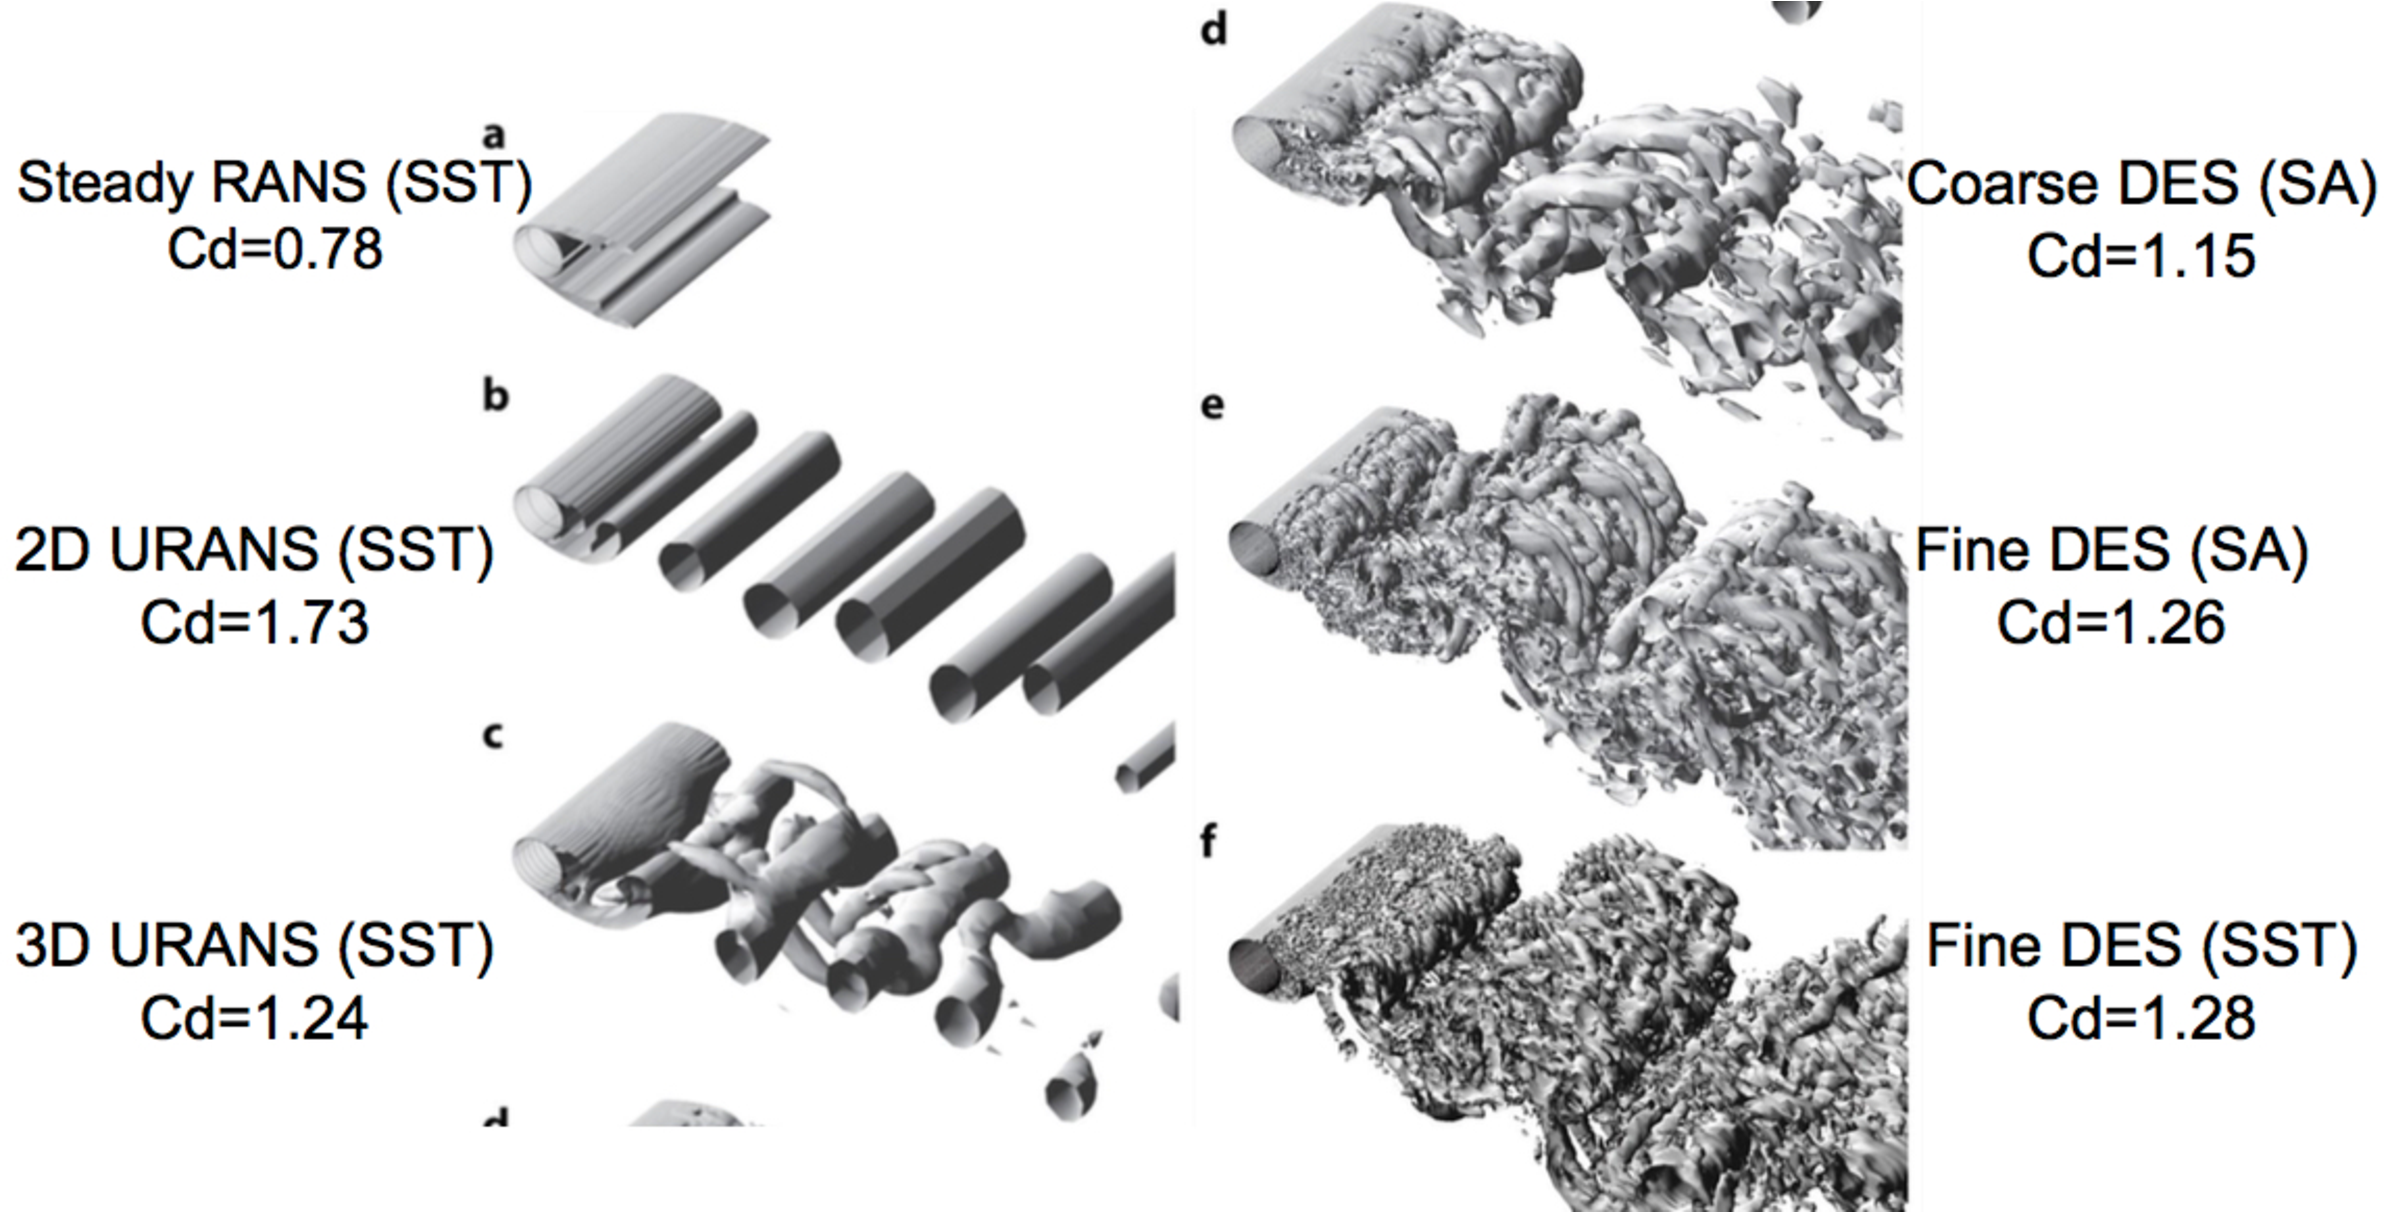
\includegraphics[width=1.0\textwidth]{Images/logan/spalart2009detachededdy_cylindersCD.pdf}
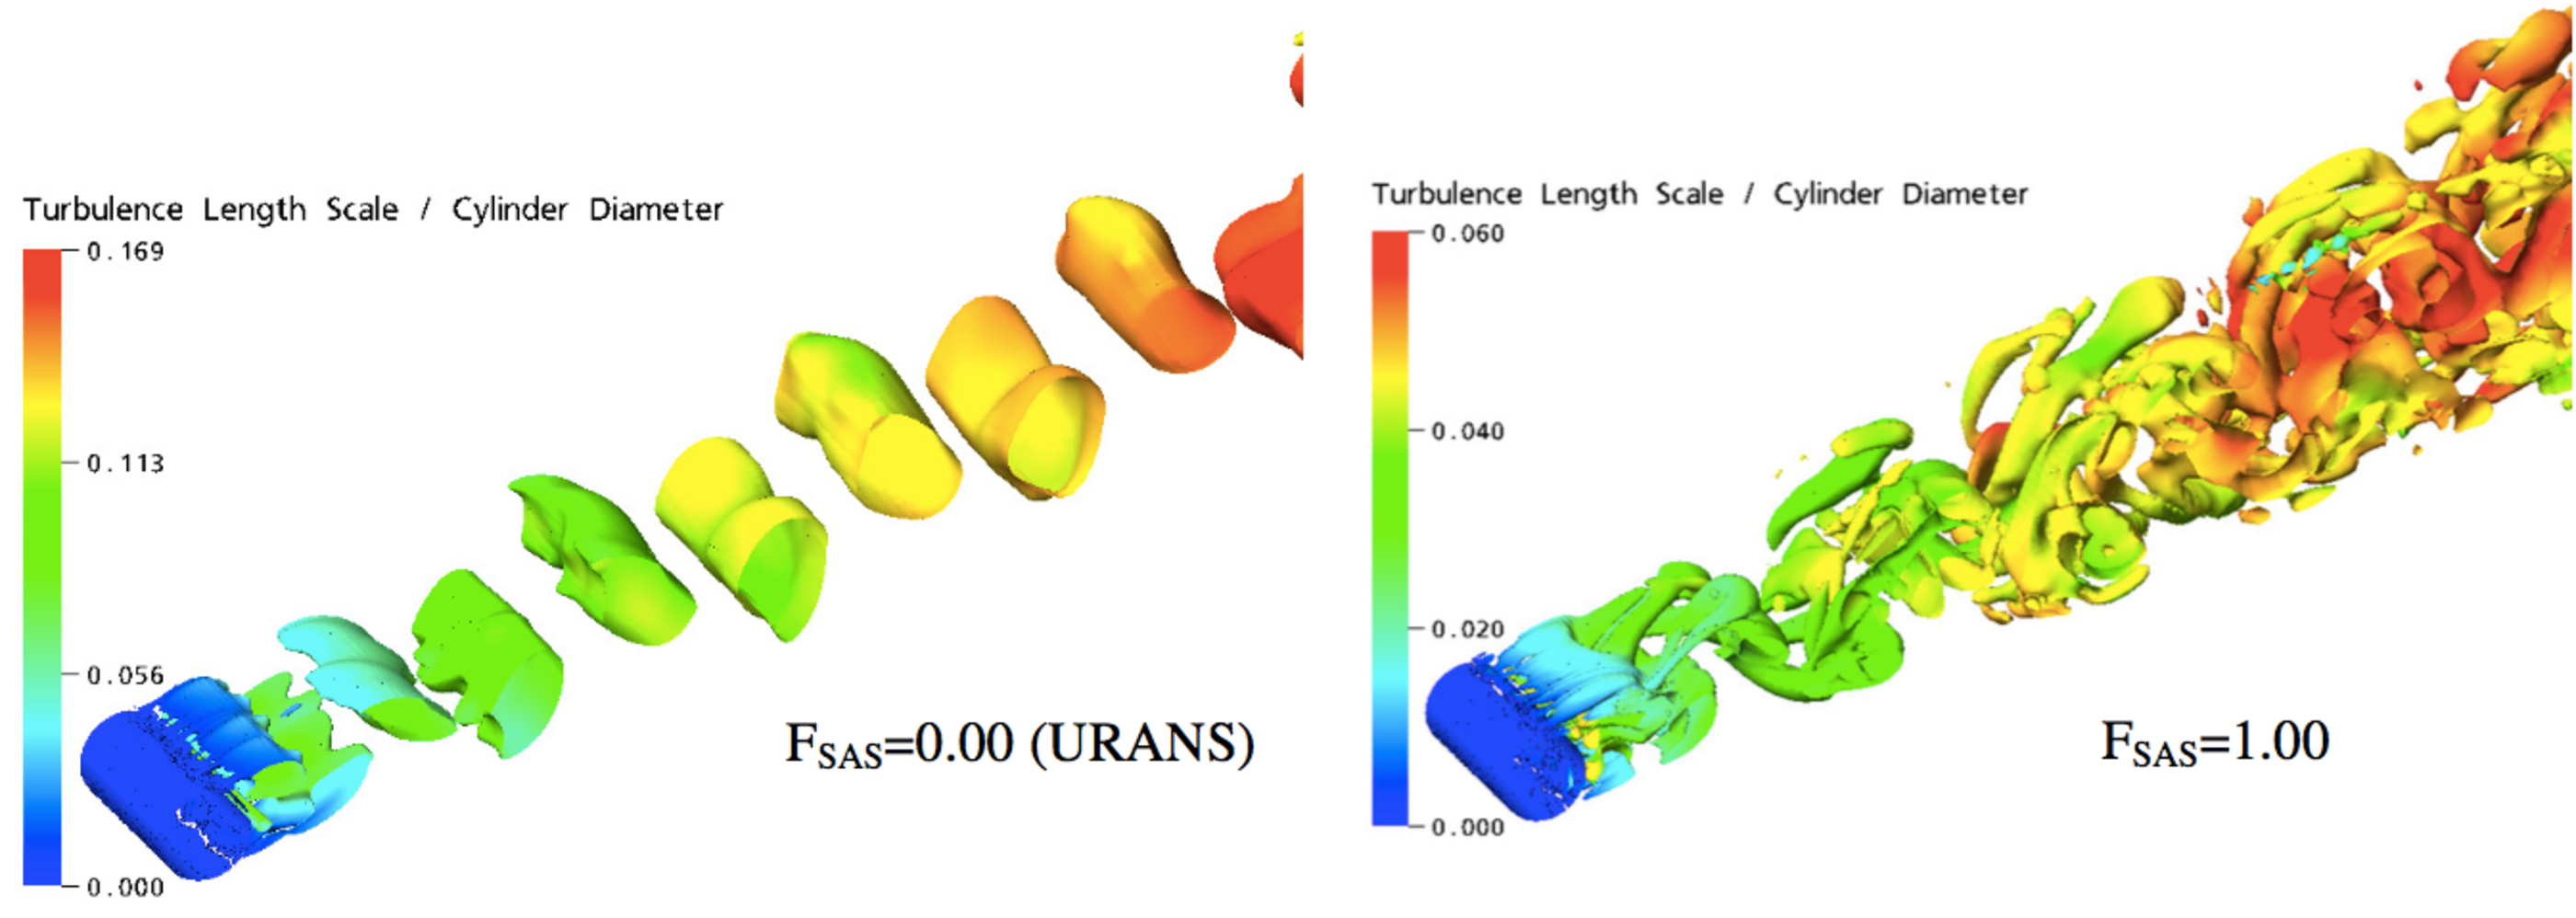
\includegraphics[width=0.65\textwidth]{Images/logan/menter2005scaleadaptive_cylinderwake.pdf}
\caption{ Comparison of wind tunnel test of a circular cylinder with drag fluctuating coefficient ranging from $C_d=1.15-1.25$ compared with time-averaged $C_d$ values from simulations using RANS (a), 2D URANS (b), 3D URANS (c), DES-SA on a coarse grid (d), DES-SA on a fine grid (f), and DES-SST on a fine grid (e) \cite{spalart2009detachededdy} in black and white and SAS simulations with null (left) and finite (right) adjustable length-scales in color \cite{menter2005scaleadaptive}. Visualizations are isocontours of vorticity }
\label{fig:cylinderturbmodels}
\end{center}
\end{figure}
%%\vspace{-2em}









%%%%%%%%%%%%%%%%%%%%%%%%%%%%%%%%%%%%%%%%%%%%%%%%%%%%%%%%%%%%%%%%%%%%%%%%
\subsection{Comparison of RANS and LES/DES Methodologies for Bluff-Bodies} \label{subsec:desvsrans}

Though Section~\ref{subsec:initialcompare} demonstrates that higher-fidelity CFD methodologies like LES are undoubtedly capable of more realistic, unsteady bluff-body simulation than RANS methods, the ambiguity of the accuracy of time-averaged results for each method calls for further comparison of the strengths and weaknesses of URANS and LES/DES in predicting time-averaged quantities for bluff-body flows.

First, URANS will be compared directly to LES in the study by Catalano et al. (2003) \cite{catalano2003numerical} of a circular cylinder at a relatively high Reynolds number of $Re_D = 1.0 \times 10^6$. A qualitative flow comparison of the two solutions in Fig~\ref{fig:cylinderransvslesflow} demonstrates that there is a obvious difference in both the instantaneous and time-averaged flow behavior between the two methods, which is consistent with the discussion in Section~\ref{subsec:initialcompare}.



%%% LES VS RANS CYLINDER FLOW
%%\vspace{-2em}
% \begin{figure}[htb]
\begin{figure}[H]
\begin{center}
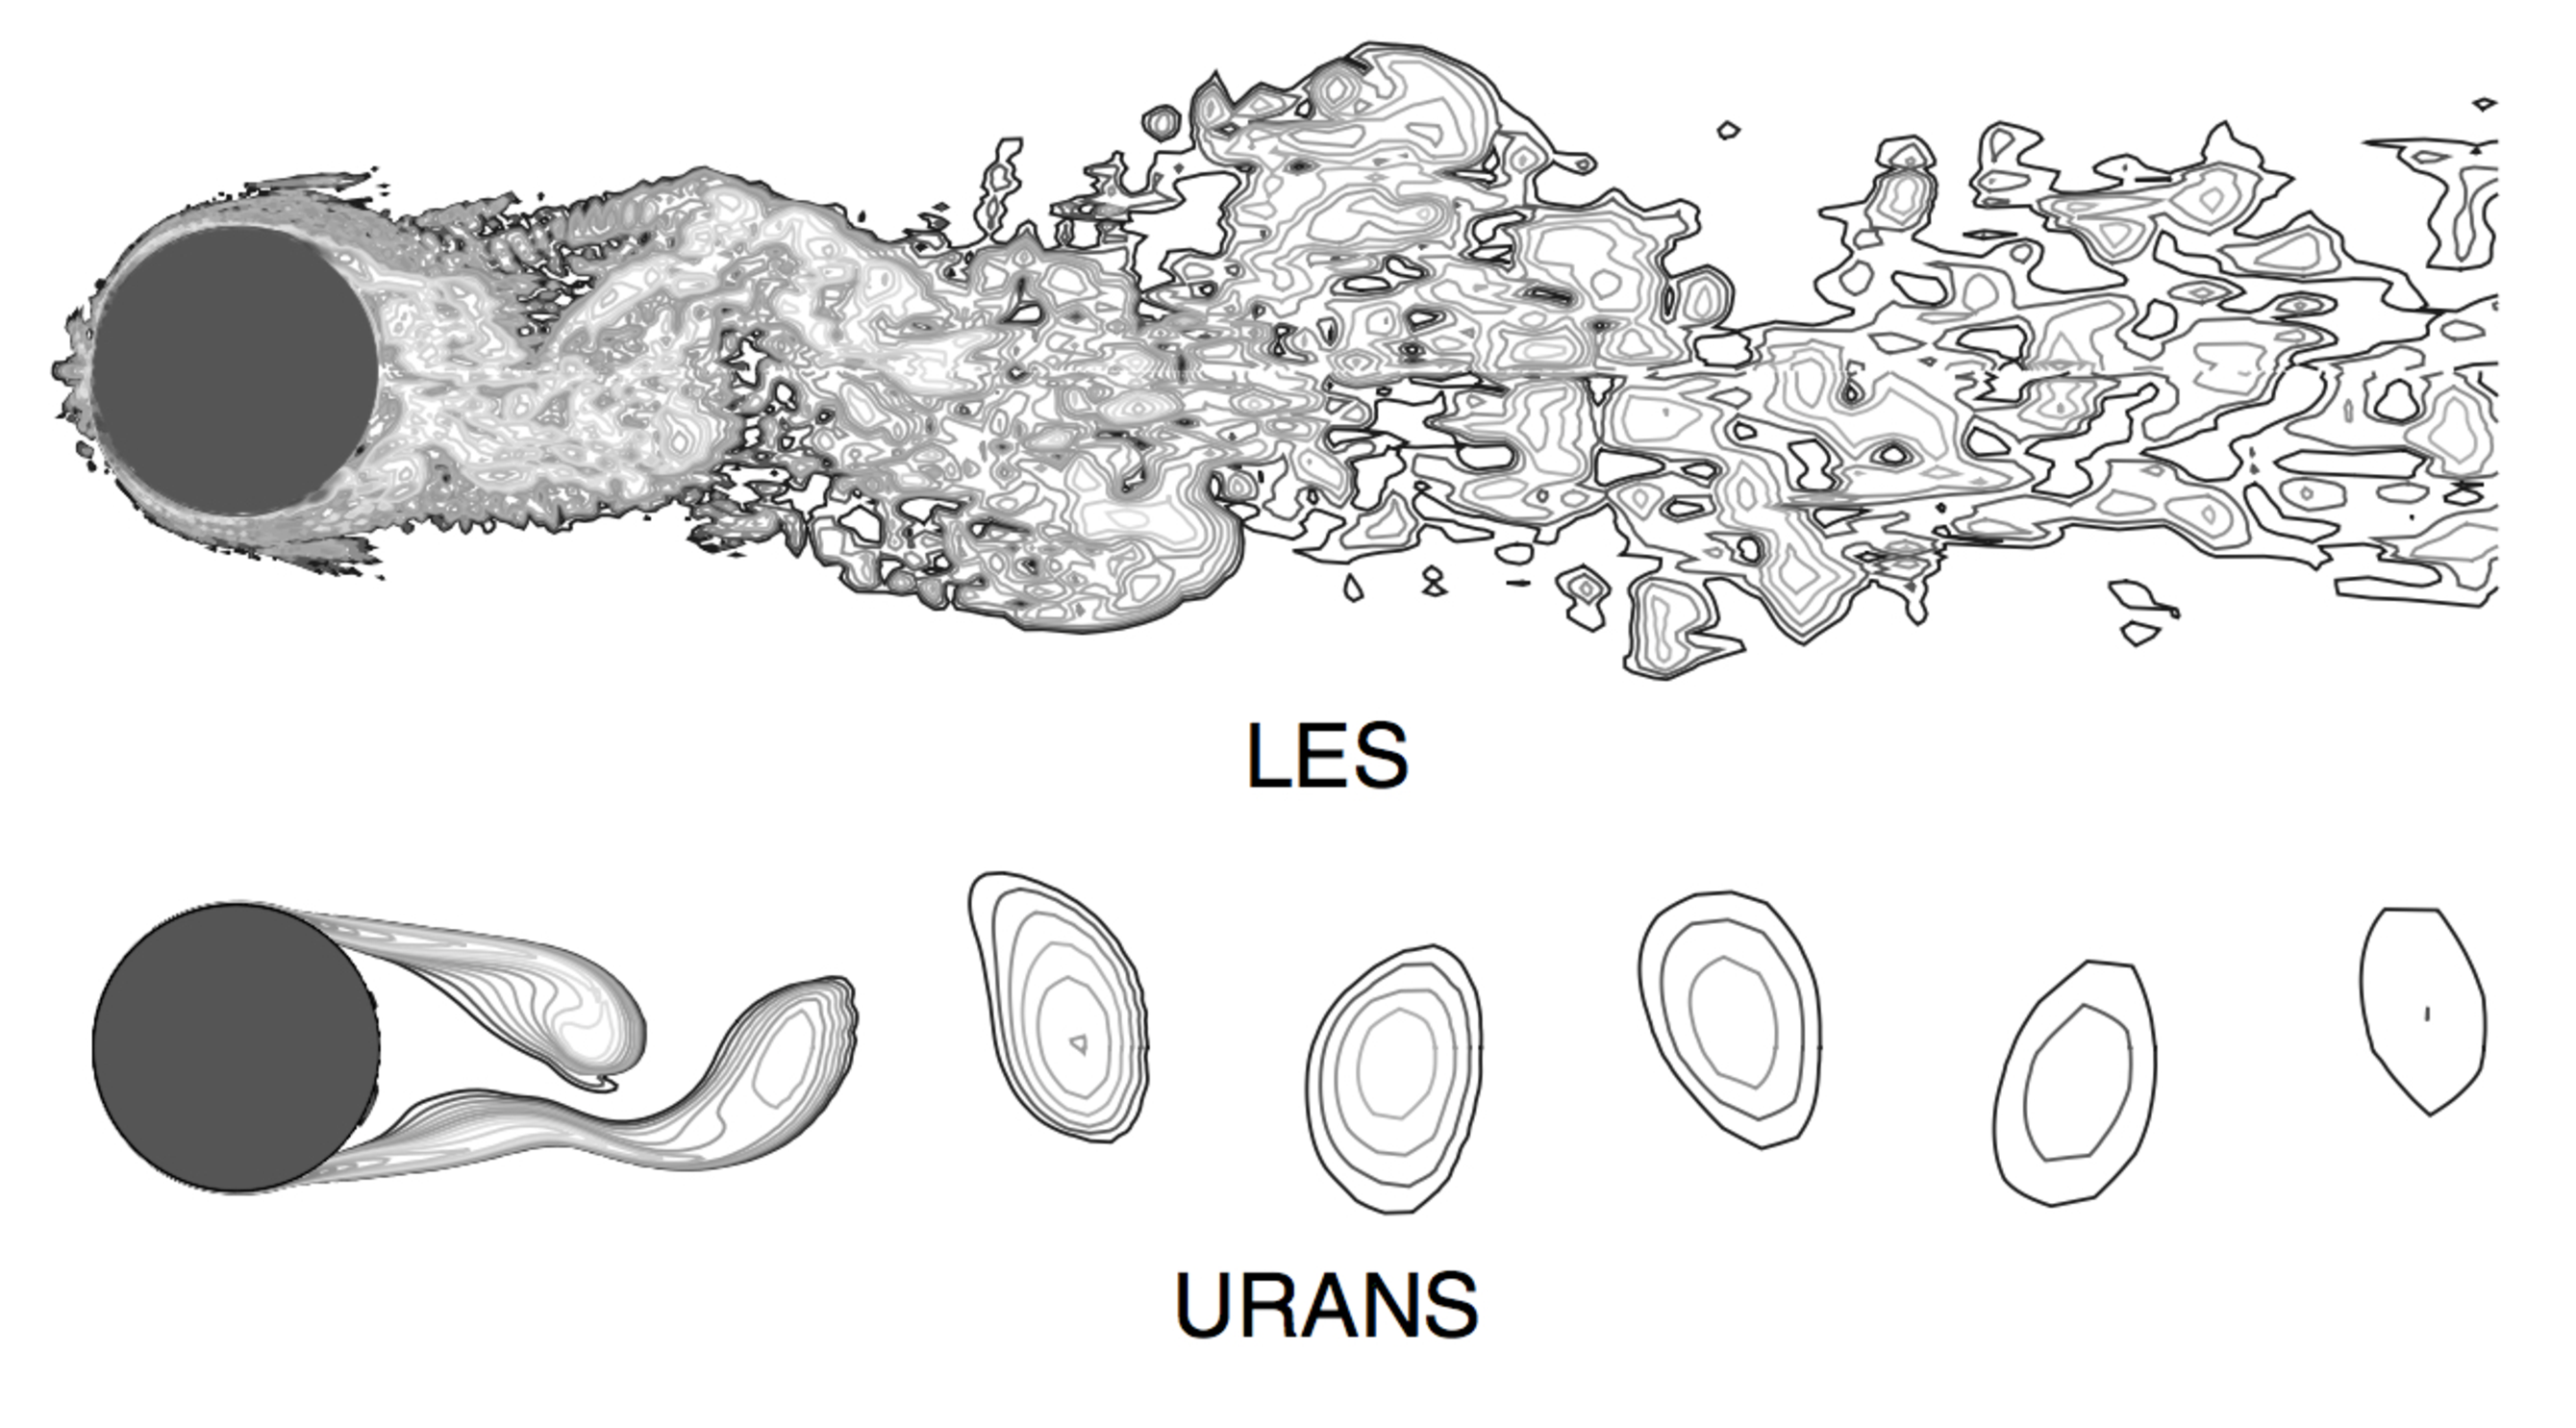
\includegraphics[width=0.45\textwidth]{Images/logan/catalano_2003numerical_UnsteadyURANSvsLES.pdf}
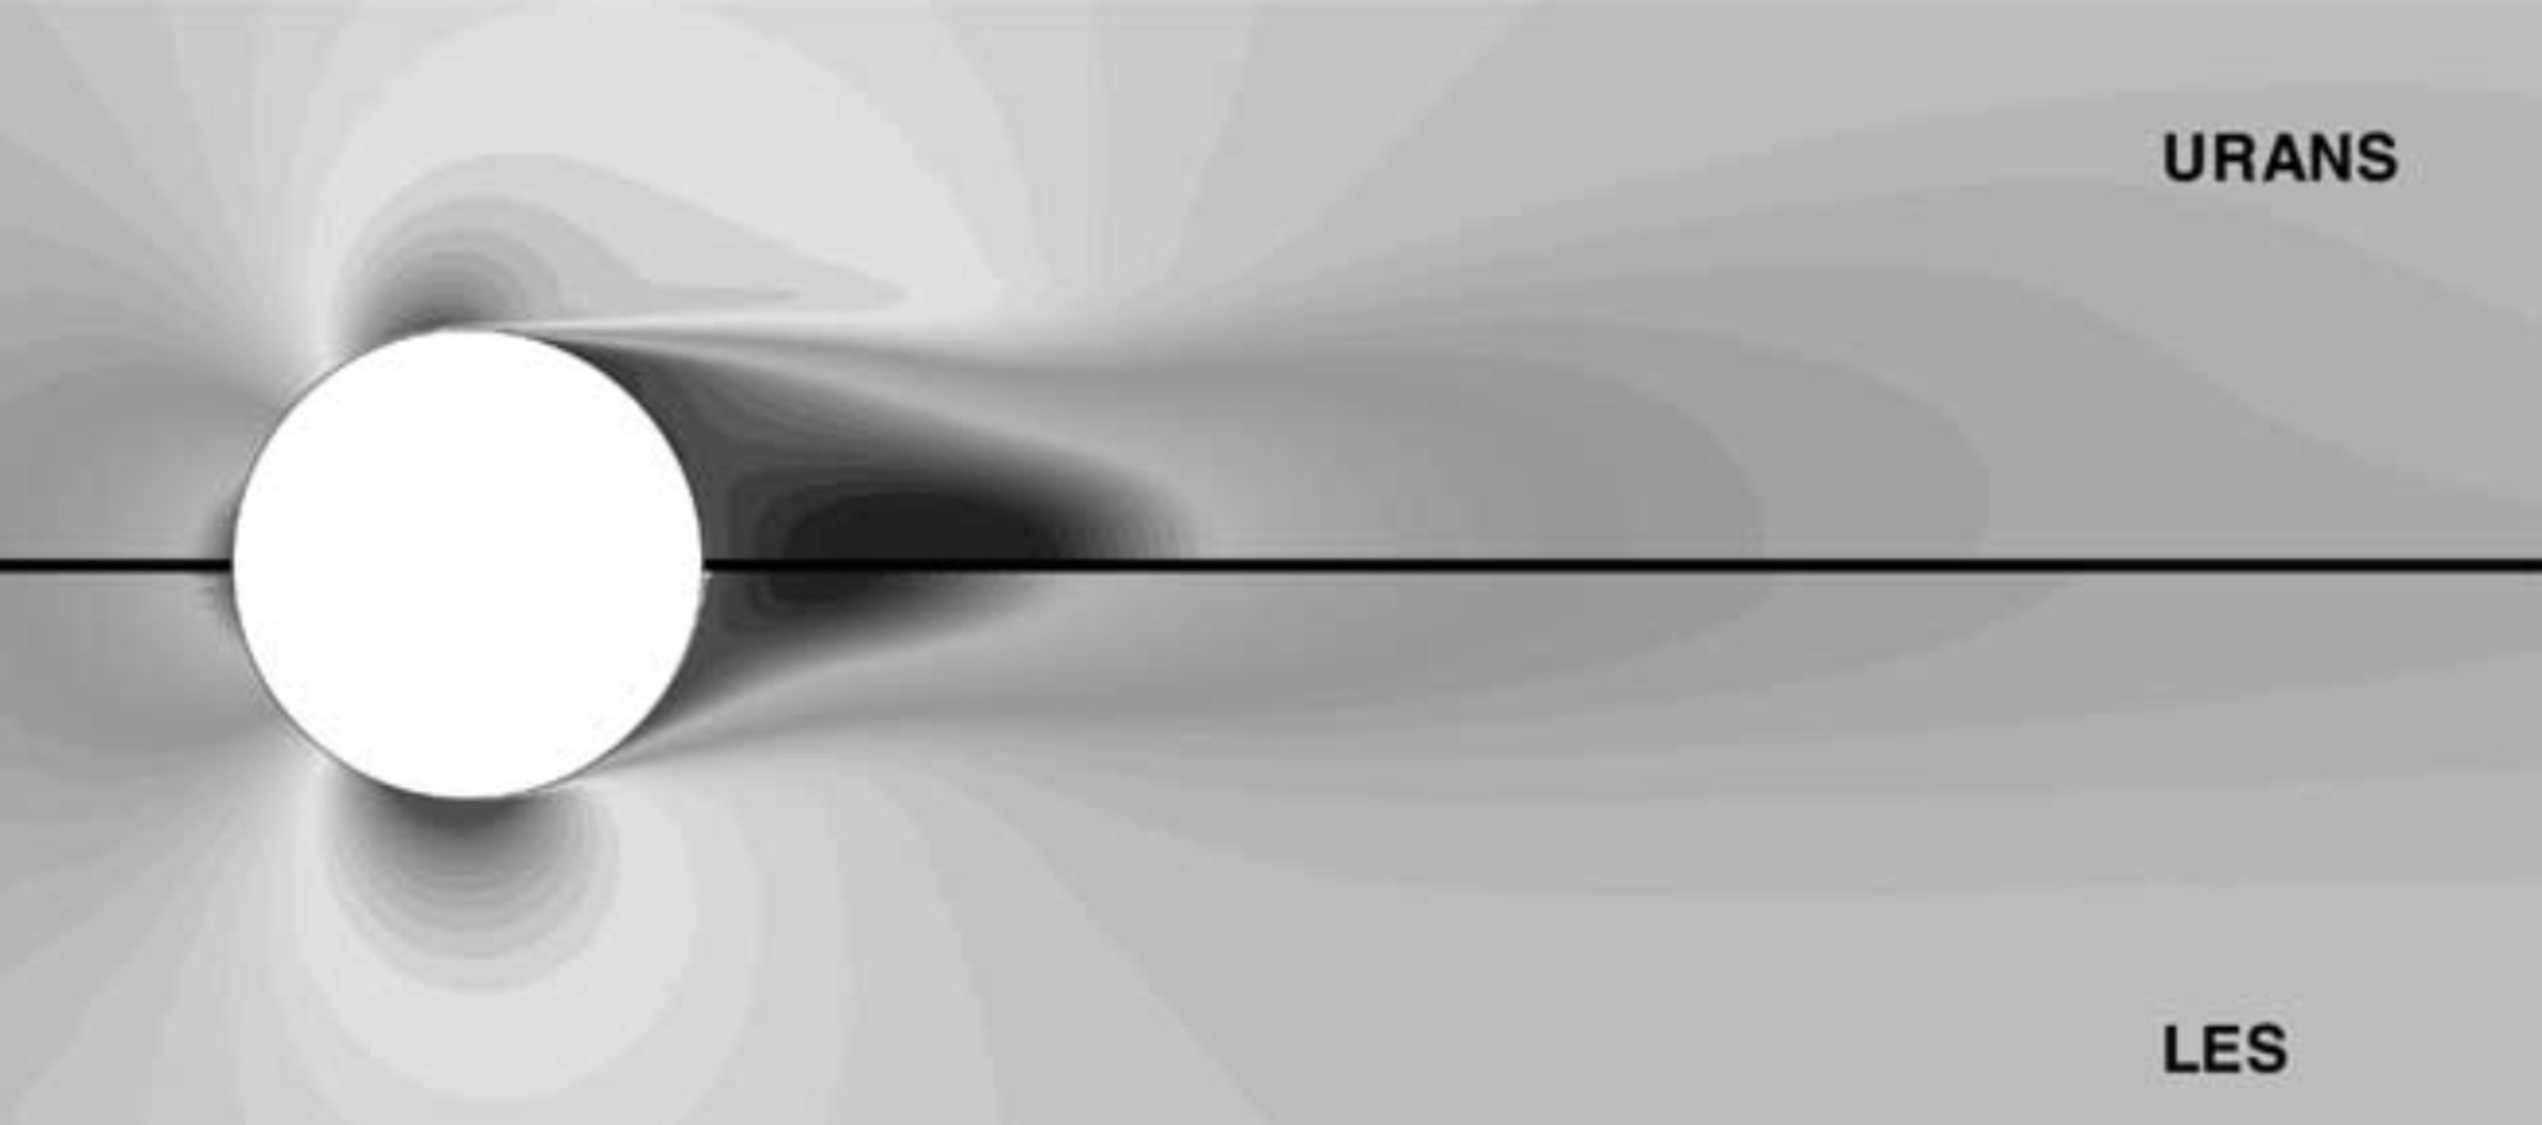
\includegraphics[width=0.54\textwidth]{Images/logan/catalano_2003numerical_SteadyURANSvsLES.pdf}
\caption{ Instantaneous vorticity magnitude (left) and time-averaged streamwise velocity distribution of numeric solutions for circular cylinder at $Re_D = 1.0 \times 10^6$ \cite{catalano2003numerical} }
\label{fig:cylinderransvslesflow}
\end{center}
\end{figure}
%%\vspace{-2em}


Quantitative comparison of the two methodologies against experiment can be found in Fig~\ref{fig:cylinderransvslesvalidation}. To the left, it can be seen that LES matches both the suction peak before separation (near $\theta=90^o$) and the constant base pressure in the separated wake ($\theta=130-180^o$) of the $Re_D = 1.2 \times 10^6$ experiment more closely than URANS. However, the advantage of LES over URANS in this application diminishes with increasing Reynolds number, since more grid refinement is required by LES to resolve finer turbulence scales. Thus, as can be seen in the right of Fig~\ref{fig:cylinderransvslesvalidation}, URANS begins to predict drag coefficient more correctly at higher Reynolds numbers using the same computational resources as the $Re_D = 1.2 \times 10^6$ case.





%%% CYLINDER RANS VS LES VALIDATION
%%\vspace{-2em}
% \begin{figure}[htb]
\begin{figure}[H]
\begin{center}
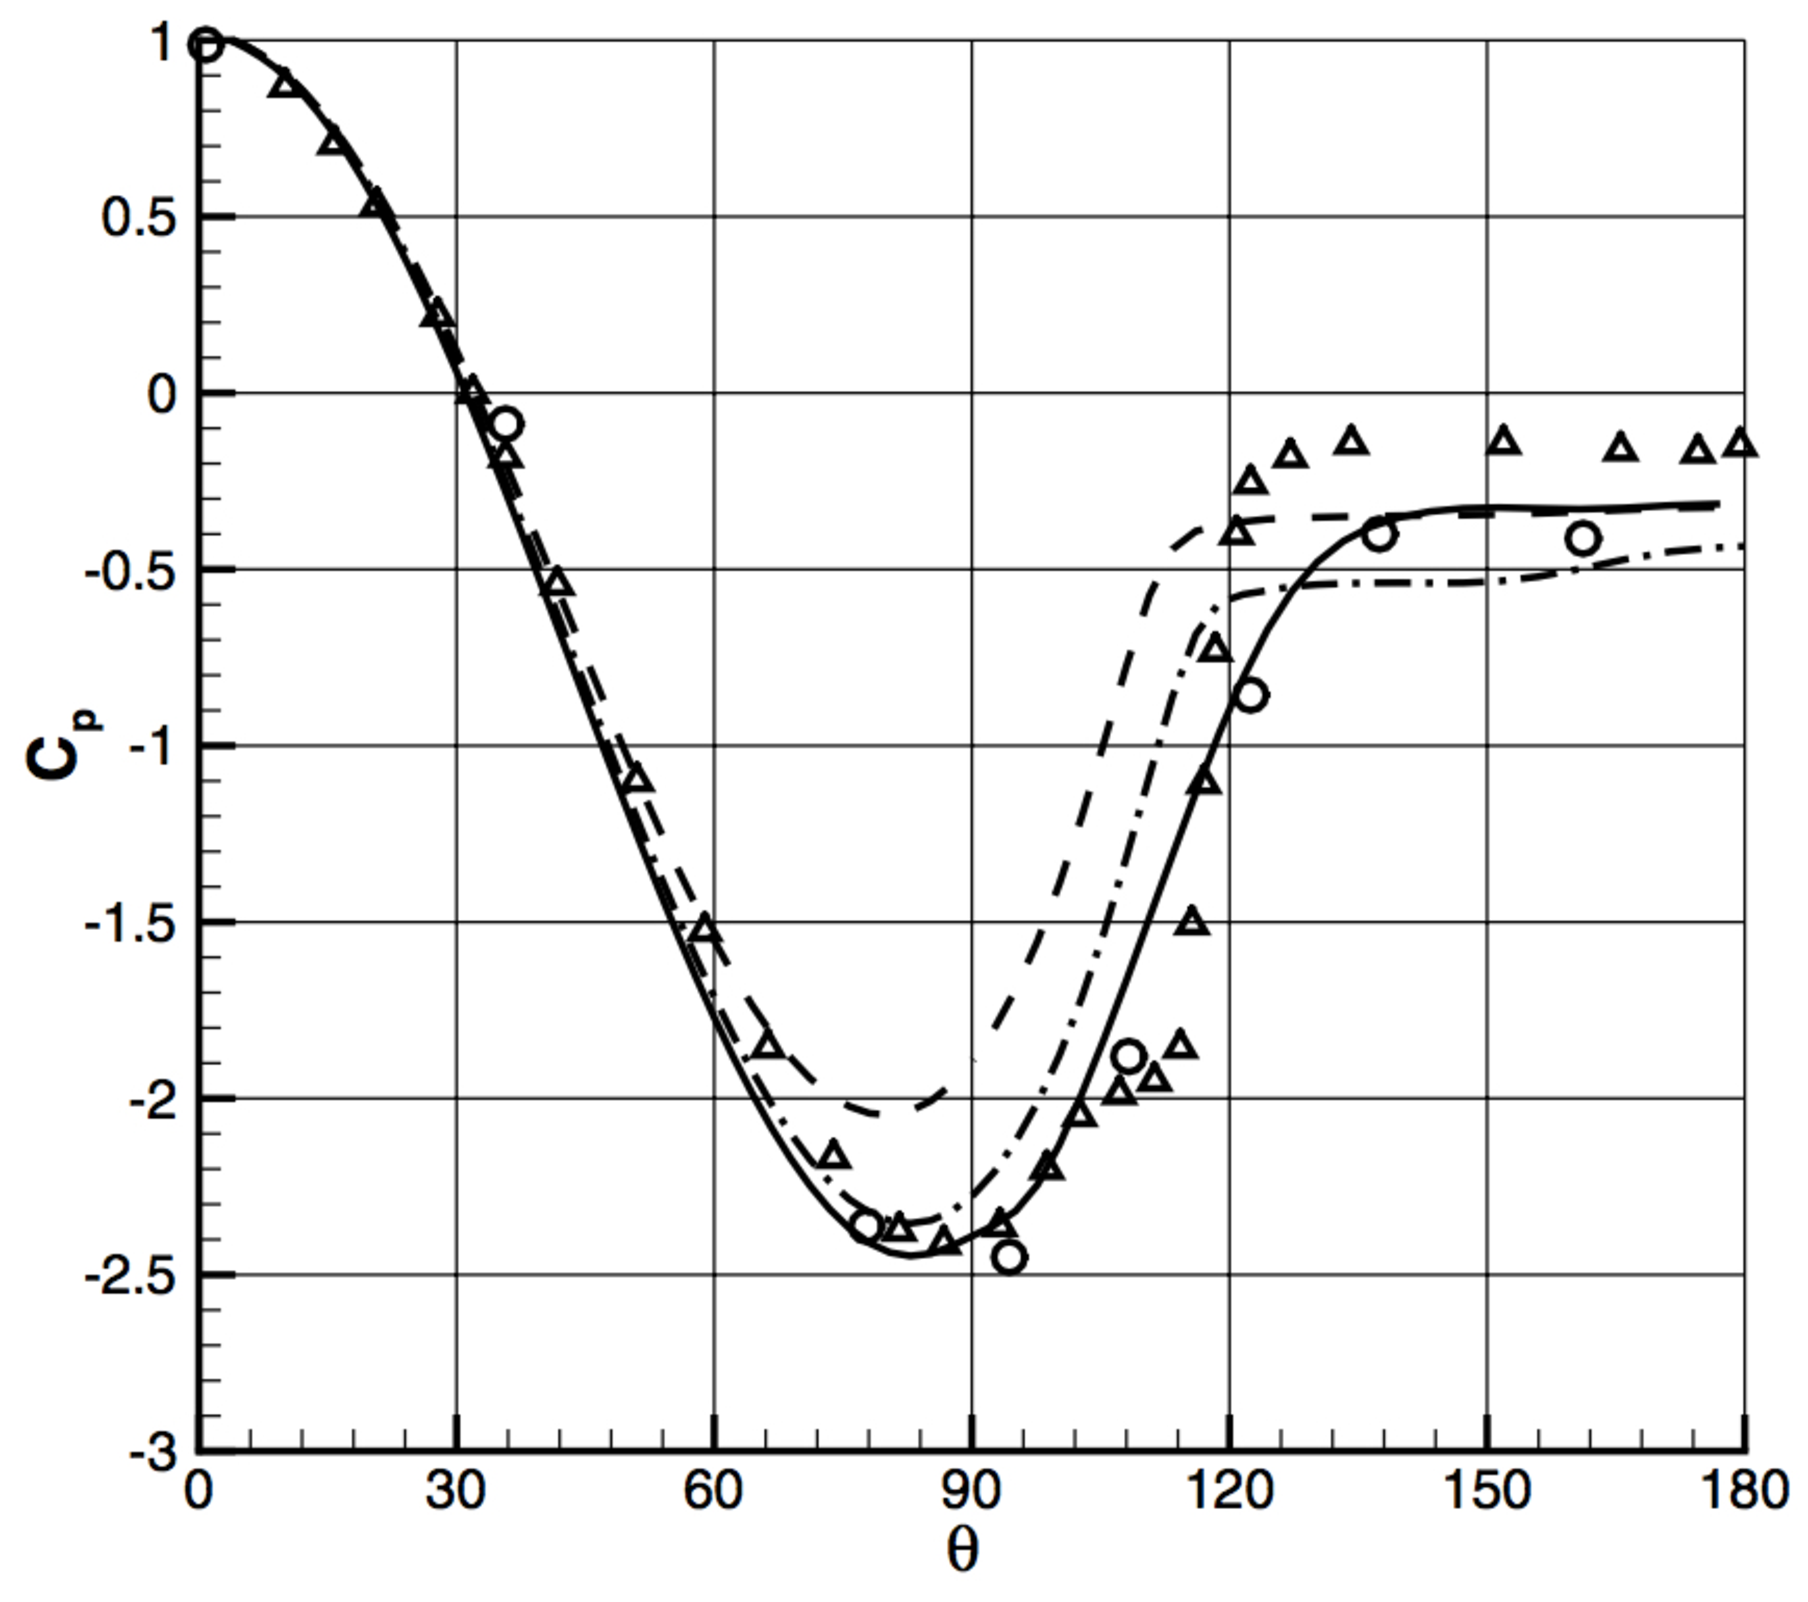
\includegraphics[width=0.49\textwidth]{Images/logan/catalano2003numerical_CylinderCp.pdf}
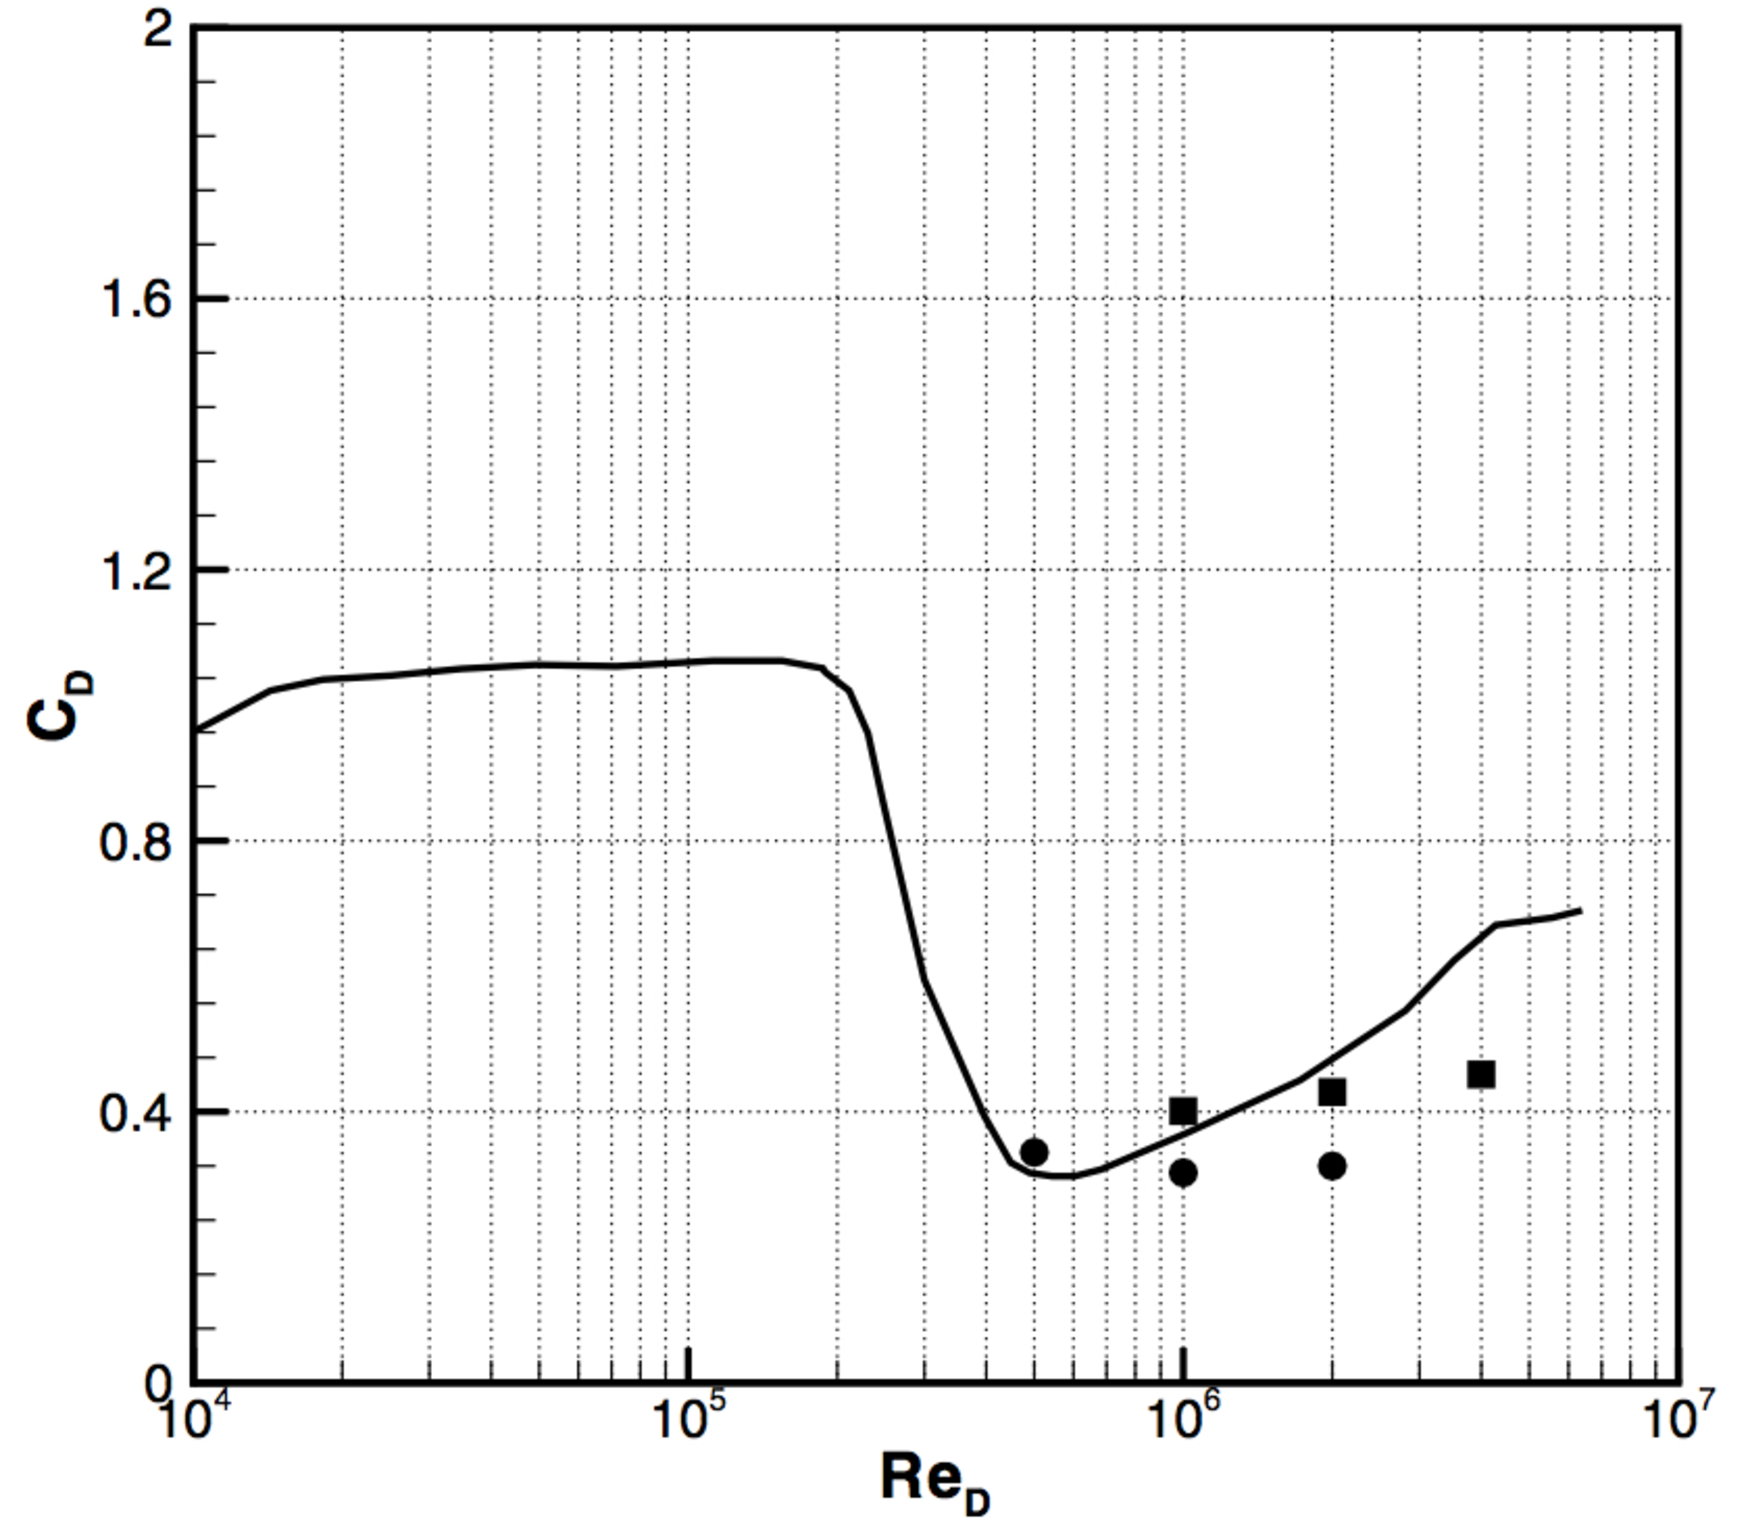
\includegraphics[width=0.49\textwidth]{Images/logan/catalano2003numerical_CylinderDrag.pdf}
\caption{ Mean surface pressure distribution on a cylinder (left) for computational methods: (---) LES, (- -) RANS, (-.-) URANS at $Re_D = 1.0 \times 10^6$ and experiments at (o) $Re_D = 1.2 \times 10^6$ and ($\triangle$) $Re_D = 6.7 \times 10^5$ and computed cylinder drag coefficient as a function of Reynolds number (right) for (--) experiment, (o) LES, and ($square$) URANS \cite{catalano2003numerical} }
\label{fig:cylinderransvslesvalidation}
\end{center}
\end{figure}
%%\vspace{-2em}


The results of this study suggest that the undisputed superiority of LES over URANS in resolving instantaneous turbulence of bluff-bodies can remain an advantage in accuracy even when time-averaging is applied. However, this conclusion is case-specific, as URANS can prevail in mean flow prediction accuracy when the flow exceeds the resolution of the LES grid due to the greater computational cost of LES.




















%%% CAPSULE DES VS RANS VS WIND TUNNEL
%%\vspace{-2em}
% \begin{figure}[htb]
\begin{figure}[H]
\begin{center}
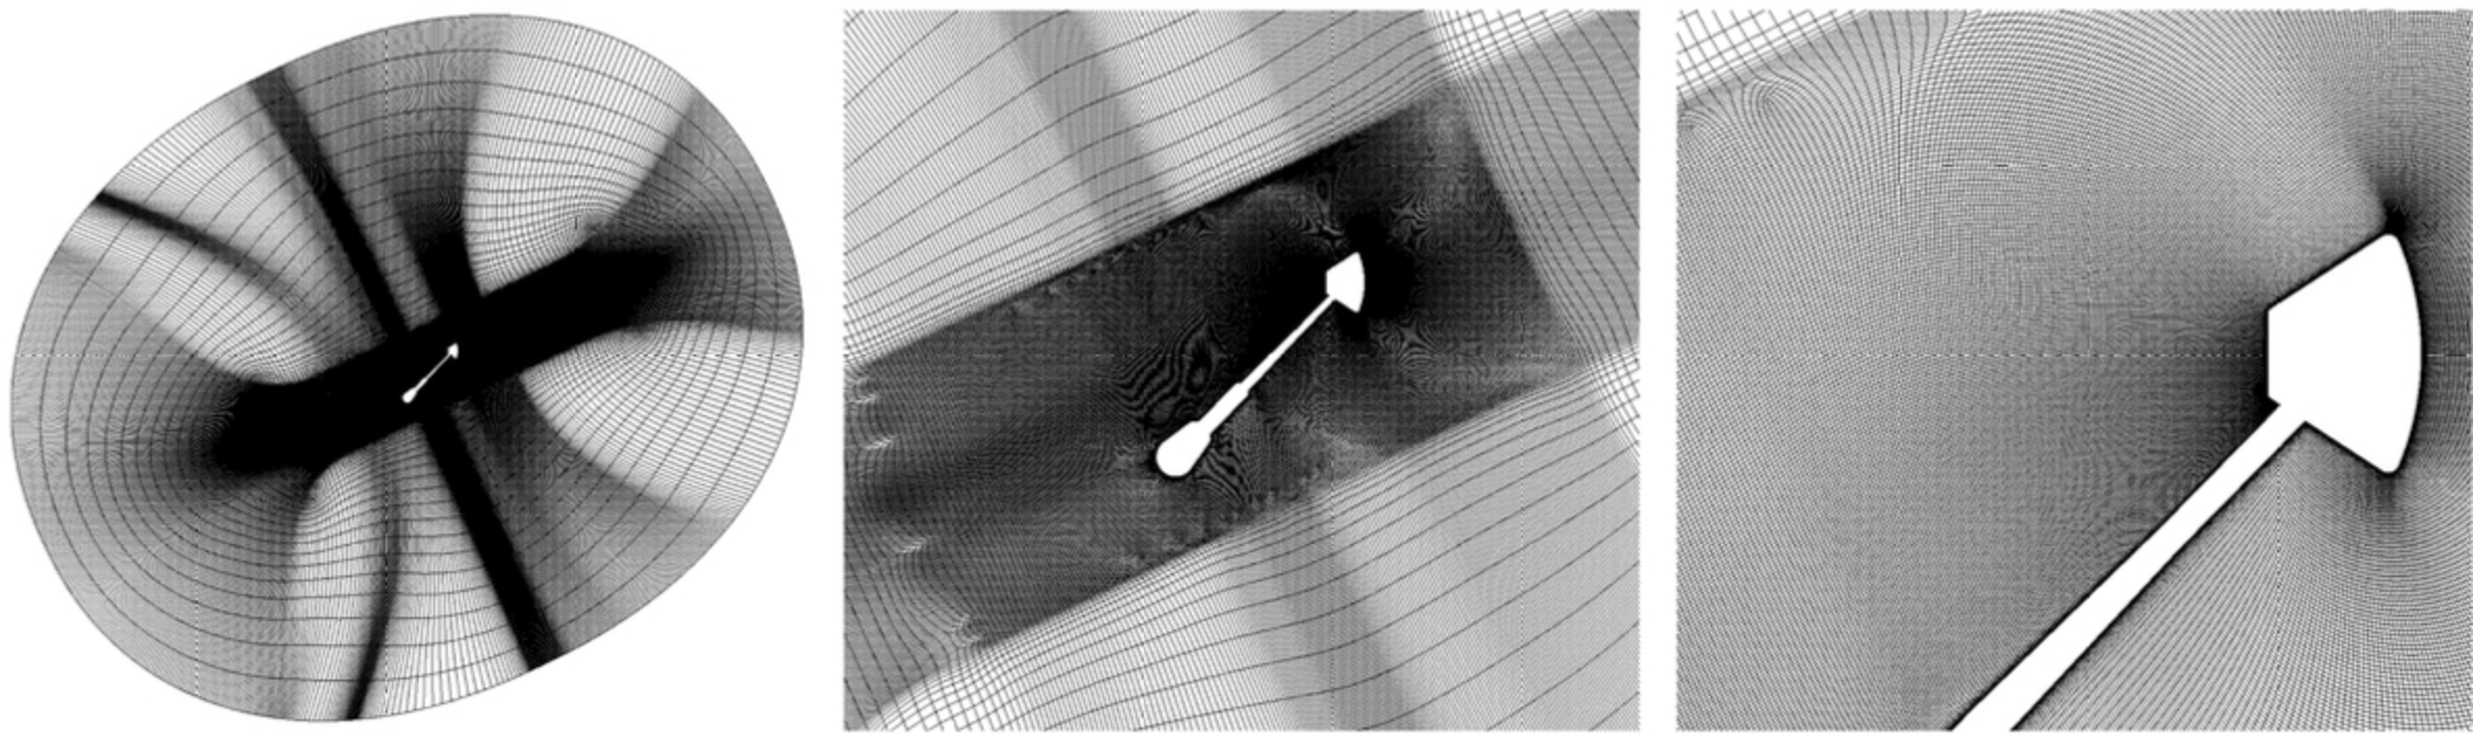
\includegraphics[width=0.95\textwidth]{Images/logan/schwing2015detachededdy_grid.pdf}
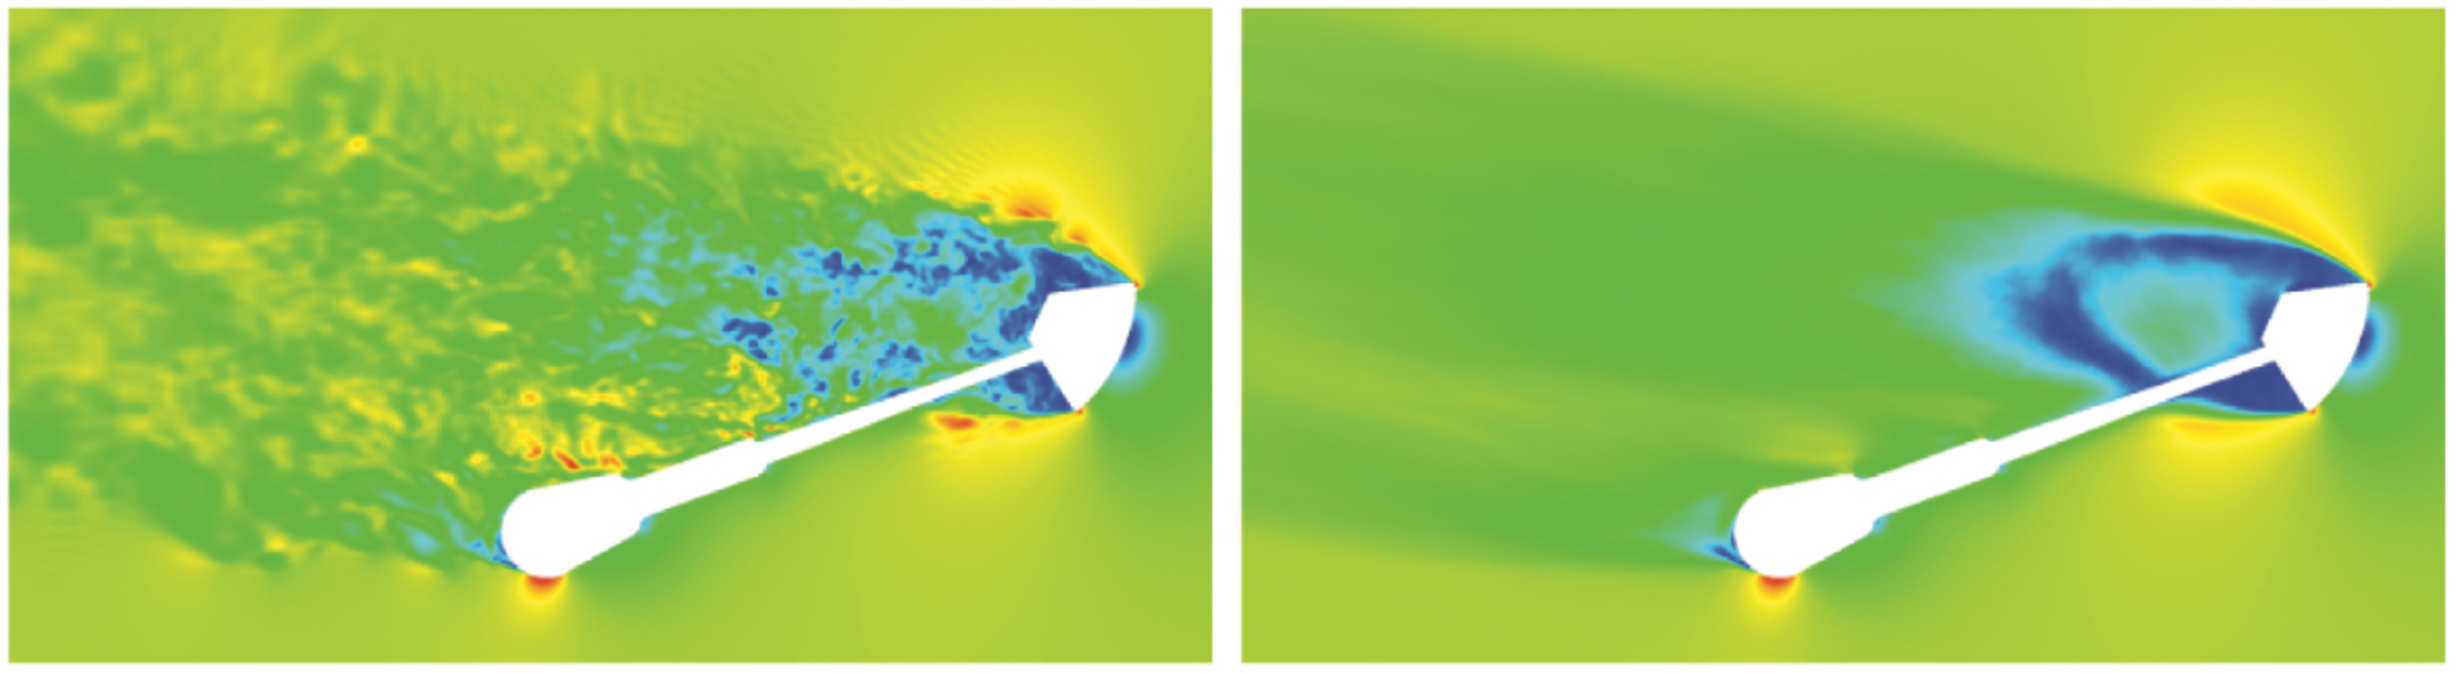
\includegraphics[width=0.95\textwidth]{Images/logan/schwing2015detachededdy_flow.pdf}
\caption{ Orion capsule and wind tunnel sting unstructured grid and instantaneous (left) time-averaged (right) Mach number (DES, $M_{\infty
}=0.5$) \cite{schwing2015detachededdy} }
\label{fig:oriongridflow}
\end{center}
\end{figure}
%%\vspace{-2em}

Next, the functionality of DES (a close sibling to LES with less computational demand) will be compared to URANS for the applied bluff-body case of an atmospheric reentry capsule during the subsonic portion of its trajectory at notably high $Re=5.0 \times 10^6$.  The study by Schwing et al. (2009) \cite{schwing2015detachededdy} compared DES and URANS simulations of the Orion capsule at subsonic and transonic Mach numbers to wind tunnel pressure data. Analysis of the prediction of both the instantaneous and mean turbulence features was performed in the study, but this review will focus on the accuracy of the simulations with regards to the time-averaged results during subsonic flight.

The mean surface pressure results for each CFD method are presented in the top image of Fig~\ref{fig:orionpressure} for $\alpha=155^o$ and are compared to the mean pressures measured by the taps in the wind tunnel test. In this example, it is obvious that the DES-KES method (which will be referred to as DES for the remainder of this section) predicts the backshell pressure distribution with vastly superior accuracy to its URANS equivalent. This advantage does not occur in all tested conditions, however, as there are many cases where the less-expensive URANS formulation produces compatible pressure distributions to DES.

A more quantitative analysis of capsule wake prediction accuracy for each model is supplied in the lower image of Fig~\ref{fig:orionpressure}, which is a line plot of the surface pressure at taps along the centerline of the capsule's cross-section. Here, two suction peaks can be seen near X/D=0.75, which correspond to the flow separation at the capsule shoulder that can be seen in Fig~\ref{fig:oriongridflow}. The magnitude of each of these peaks is most closely predicted by DES. In addition, the nearly constant base pressure on the backshell of the capsule in the separated wake is very accurately predicted by DES, while the URANS equivalent is incorrect in both magnitude and in its varying nature.  These differences in wake behavior prediction result in a much more accurate drag prediction by DES in comparison to wind tunnel results. However, DES was not the overall victor in mean load prediction since the integration of lift of for the URANS pressure distribution proved to be more accurate. The author attributes this discrepancy to separation prediction, which highlights the potential ambiguity of hybrid RANS/LES behavior in response to grid and geometry.






%CAPSULE SURFACE PRESSURE
%%\vspace{-2em}
% \begin{figure}[htb]
\begin{figure}[H]
\begin{center}
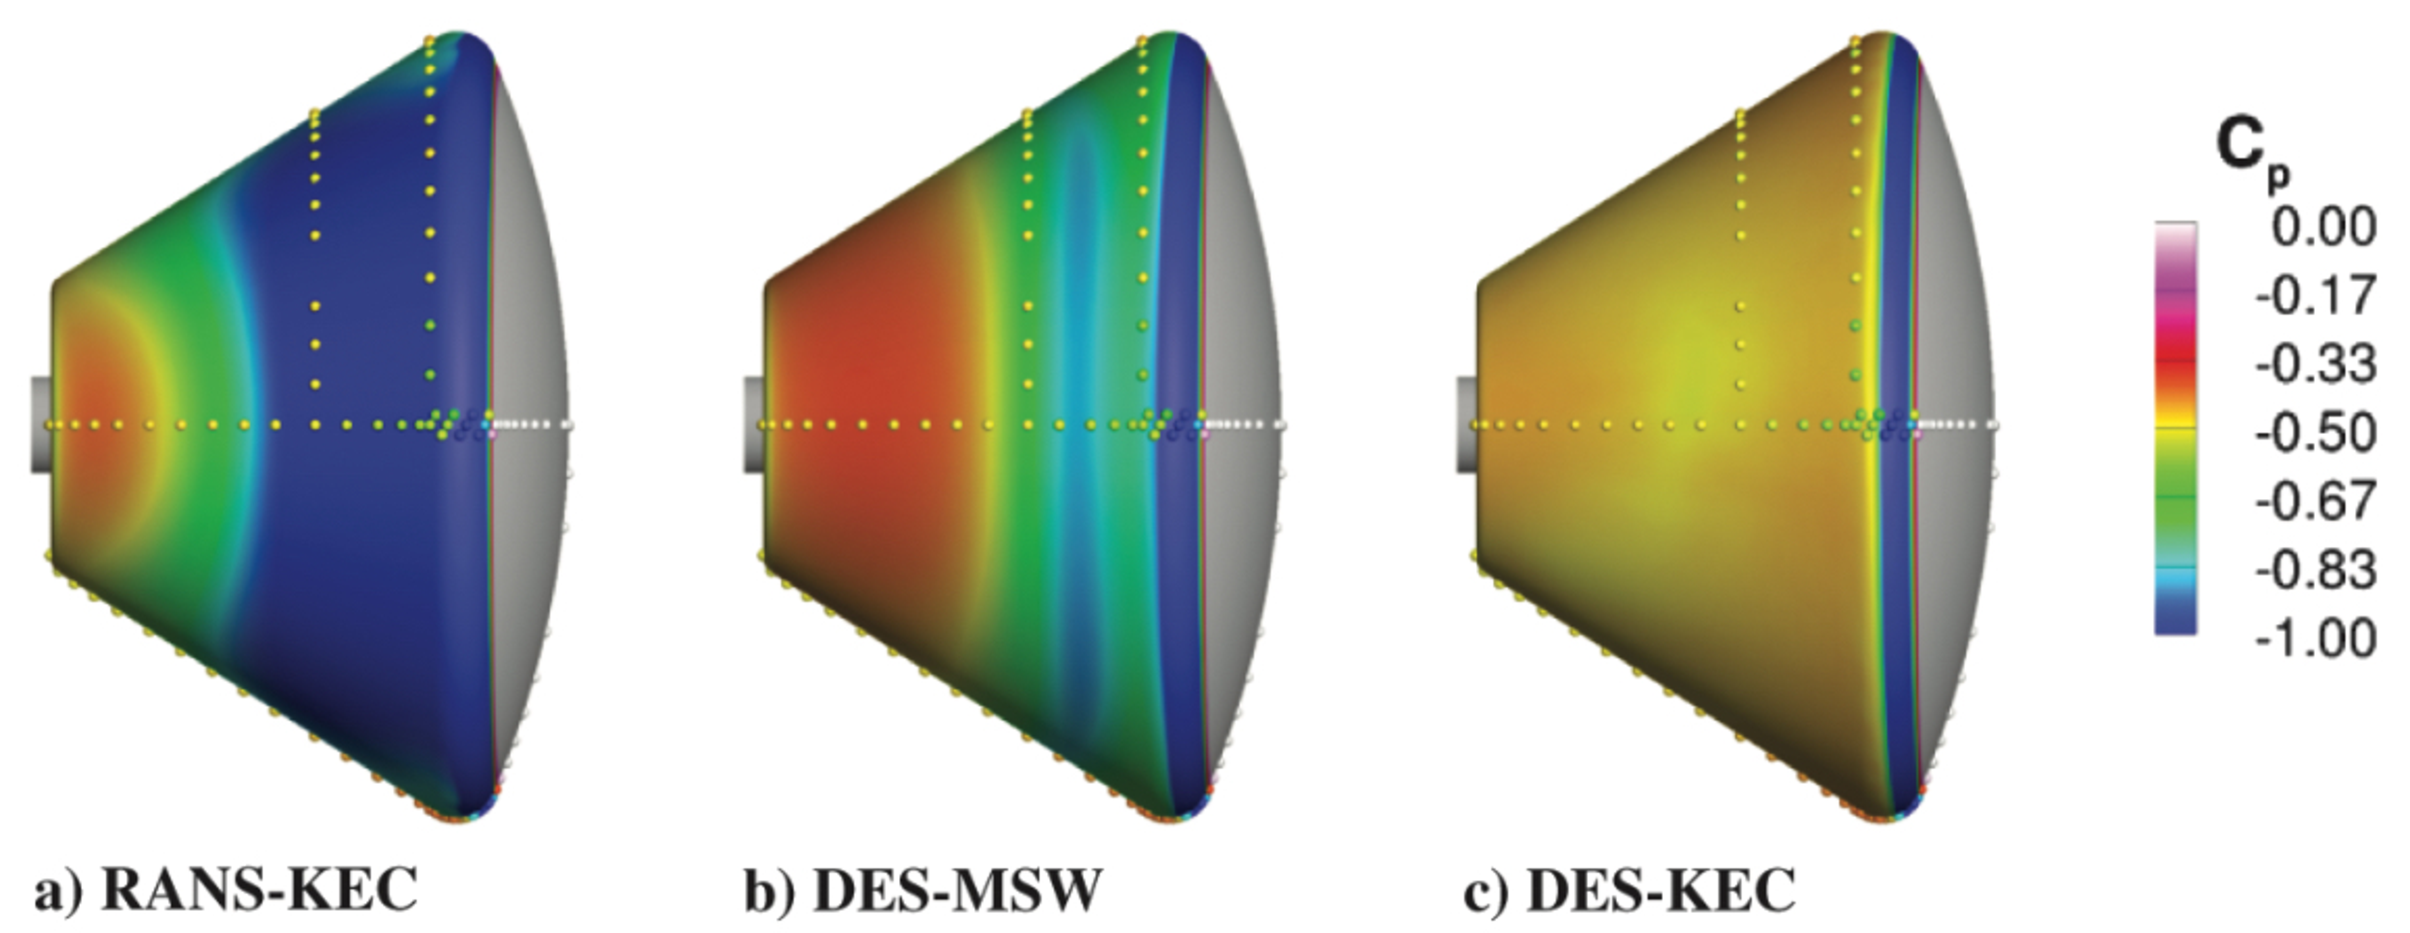
\includegraphics[width=0.95\textwidth]{Images/logan/schwing2015detachededdy_surfacepressure.pdf}
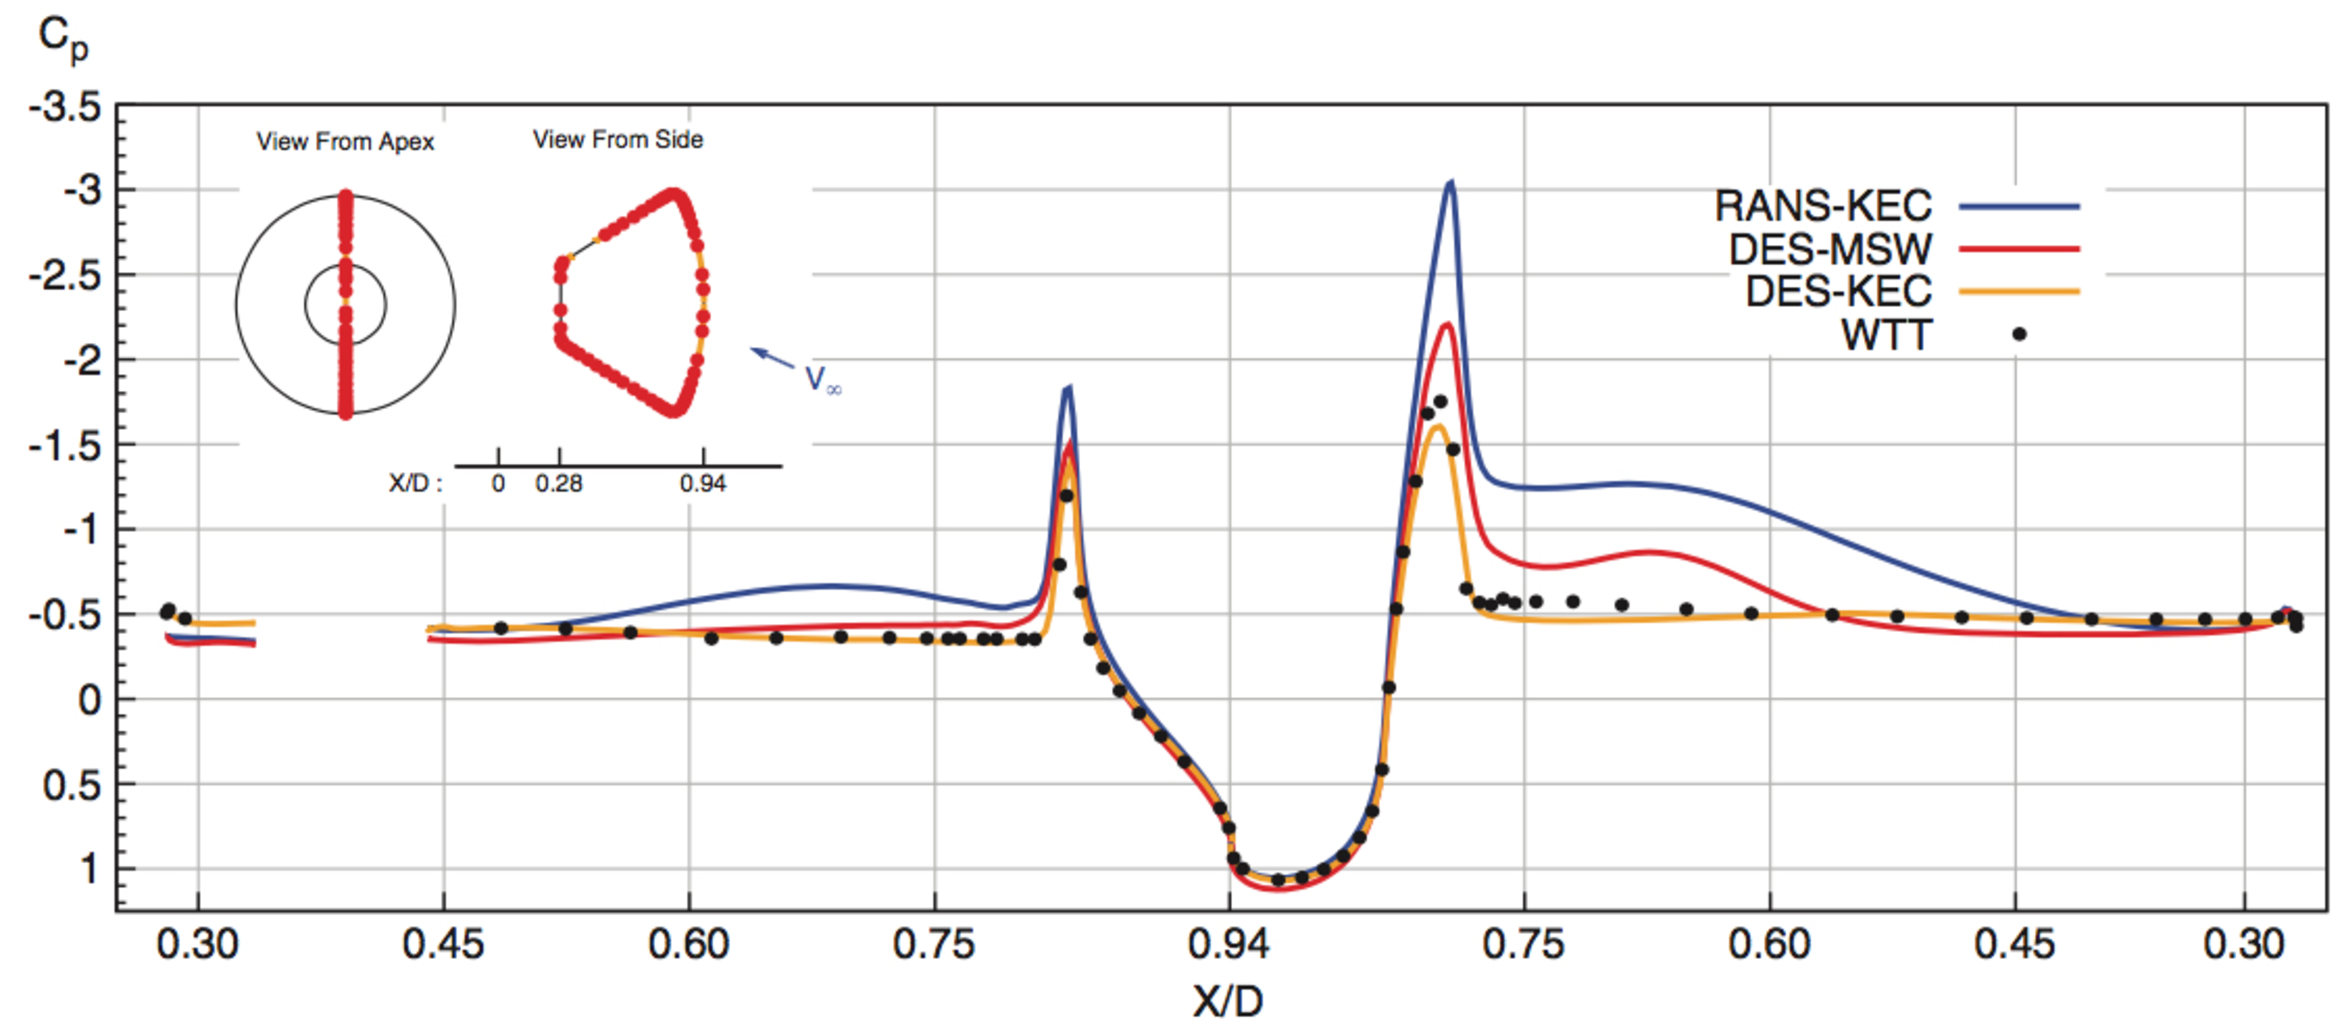
\includegraphics[width=0.95\textwidth]{Images/logan/schwing2015detachededdy_surfacetaps.pdf}
\caption{ Top: Mean simulation surface pressure contours compared to wind tunnel test (WTT) freckle plot. Bottom: Line plots of pressure tap data along a surface cross-section ($M_{\infty}=0.5,\;\alpha=155^o$) \cite{schwing2015detachededdy} }
\label{fig:orionpressure}
\end{center}
\end{figure}
%%\vspace{-2em}


The results of this study demonstrate that CFD techniques are mature enough to accurately simulate complex, realistic bluff-body flows like this high-Reynolds number reentry capsule.  Both URANS and DES proved capable in many sets of conditions, but the increased computational cost of DES became more justified at high angle of attack flight conditions where URANS was insufficient for accurate wake modeling.  The ambiguity of mean load prediction accuracy between methods demonstrates that no one method is superior for all conditions and that user intuition toward flow realism is still an essential component of an accurate bluff-body simulation.





%%%%%%%%%%%%%%%%%%%%%%%%%%%%%%%%%%%%%%%%%%%%%%%%%%%%%%%%%%%%%%%%%%%%%%%%
\subsection{Comparison of DES and SAS Methodologies for Bluff-Bodies} \label{subsec:desvssas}

It has been established in the previous sections that higher-fidelity CFD methods like LES and DES are capable of producing more realistic predictions of turbulent effects than URANS methods but that this superiority comes at the cost of significantly increased computational demand and other potential sources of inaccuracy like Grid Induced Separation, which will be discussed later. Scale-Adaptive Simulation was developed in an attempt to avoid some of these issues, so it is relevant in this study to compare the accuracy and performance of these methods in their application to bluff-bodies.

A study by Zheng et al. (2016) \cite{zheng2016comparative} compared DES and SAS simulations of flow over a circular cylinder at $Re_D = 1.4 \times 10^5$. Computations with each method were performed with the same grid resolution, and results for time-averaged streamwise velocity along the wake centerline for each method and an experimental comparison are provided in Fig~\ref{fig:cylinderdesvssas}.

%%% CYLINDER DES VS SAS VALIDATION
%%\vspace{-2em}
% \begin{figure}[htb]
\begin{figure}[H]
\begin{center}
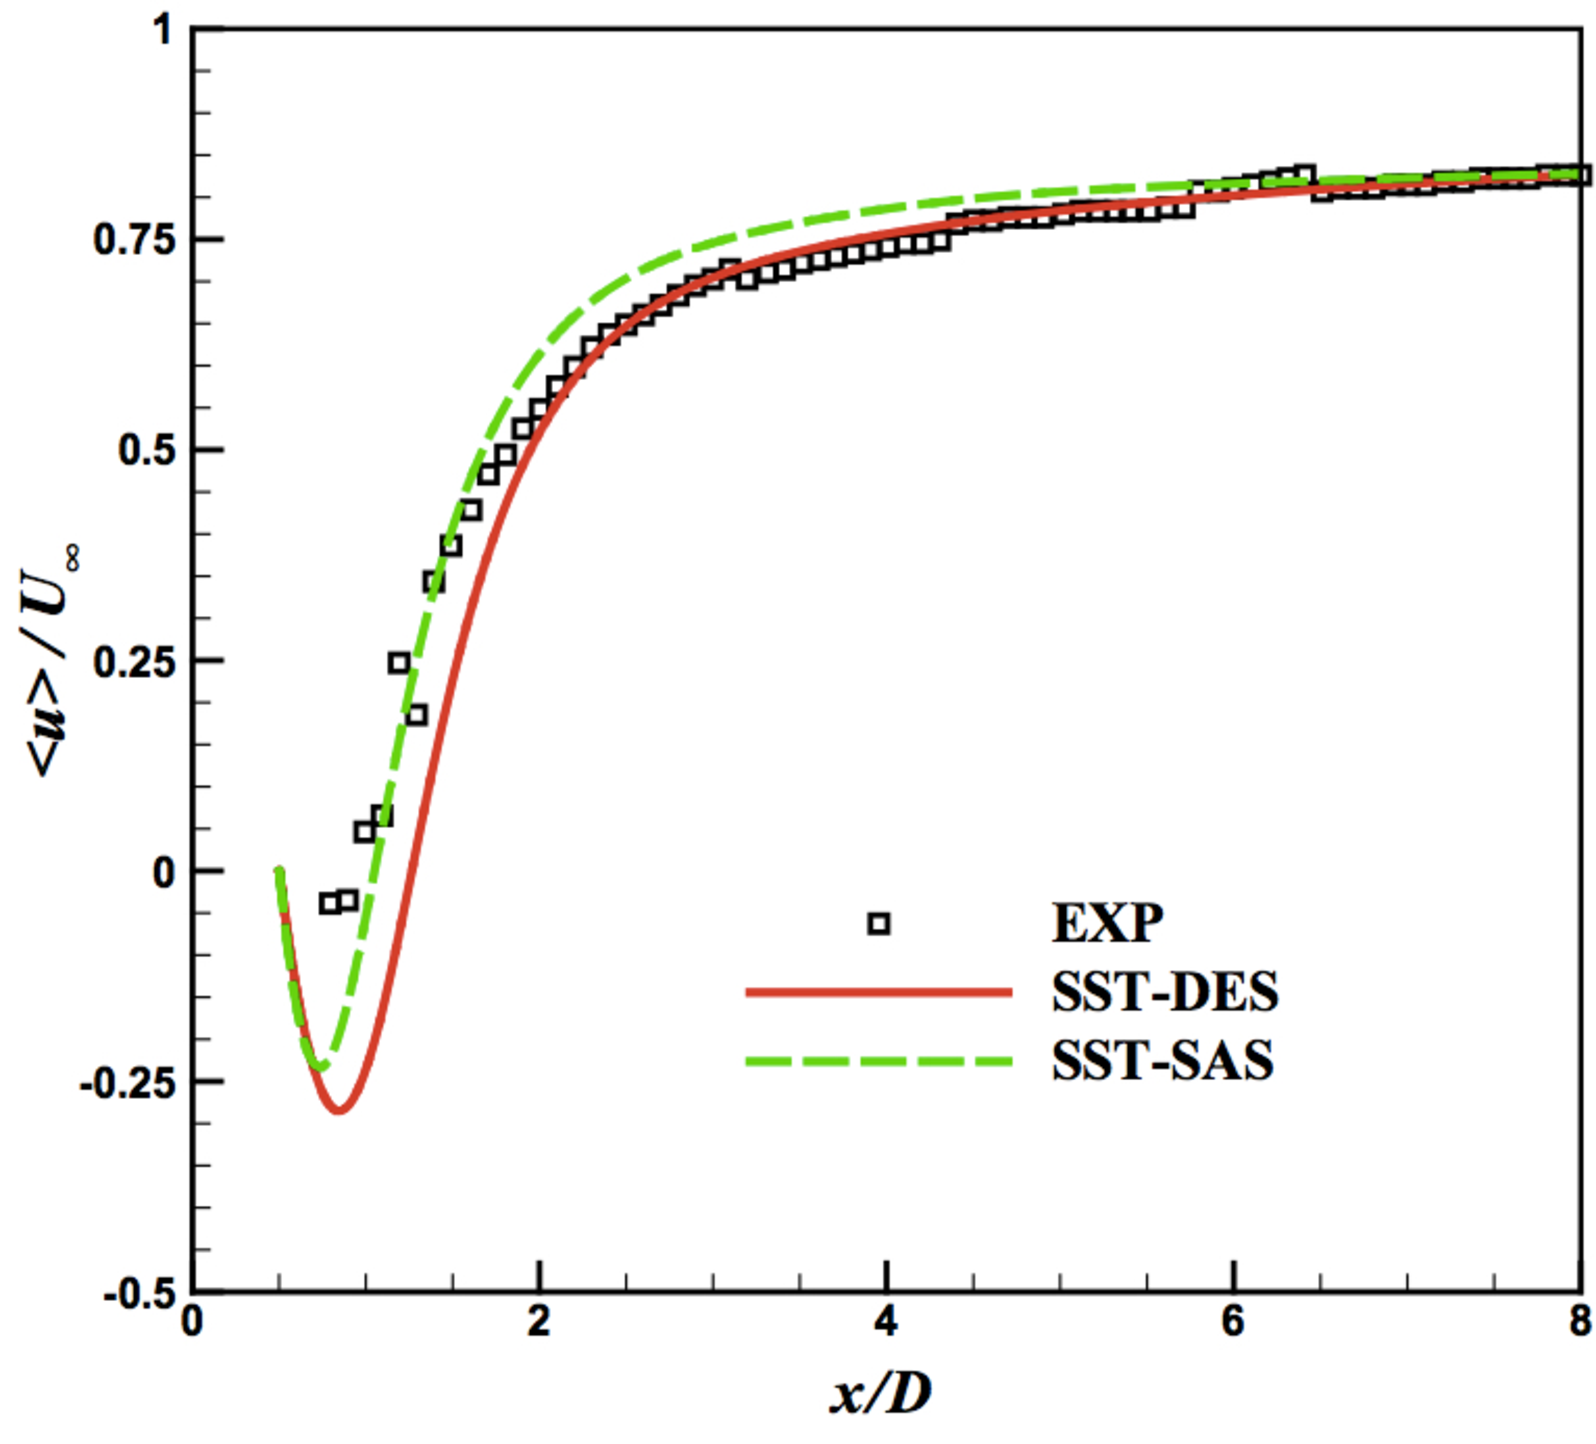
\includegraphics[width=0.49\textwidth]{Images/logan/zheng2016comparative_WakeVelocity.pdf}
\caption{ Time-averaged streamwise velocity along the wake centerline for a circular cylinder $Re_D = 1.4 \times 10^5$ \cite{zheng2016comparative} }
\label{fig:cylinderdesvssas}
\end{center}
\end{figure}
%%\vspace{-2em}

The results demonstrate that, in this application, SAS predicts flow phenomena in the near wake that are more similar to the experiment than DES, while DES becomes more accurate further downstream since SAS is more dissipative in this region. Both methods produce accurate results in the far wake. This single comparison does not necessarily demonstrate that either SAS or DES is superior to the other but rather highlights that both methods can be considered to have comparable accuracy and that each will have a unique and specific set of applications where it is superior.






It is also relevant to consider the differences in computational cost between the two methods, as this is often a limiting factor for realistic engineering tasks. A preliminary study by Wang et al. (2017) compared the simulation of flow over a high-speed train computed by URANS, SAS, and Delayed DES (an even more cost-intensive version of DES) to wind tunnel results \cite{wang2017performance}. The study found that the ratio of computational cost of the three methods URANS:SAS:DDES was on the order of 1:10:20. URANS was found to have inferior accuracy to the other two methods, and DDES was found to have slightly improved results compared to SAS. This study represents an extreme case of cost differences between SAS and DES, but shows that SAS can be used as a cost-saving alternative to DES in the correct applications.
















%%%%%%%%%%%%%%%%%%%%%%%%%%%%%%%%%%%%%%%%%%%%%%%%%%%%%%%%%%%%%%%%%%%%%%%%
\subsection{Current State of Computational Methods for Bluff-Body Flows} \label{subsec:currentstatenumeric}


The relative differences between CFD methodologies has been reviewed in the previous sections. This section will detail the current state-of-the-art in bluff-body flow modeling and the challenges that remain to be addressed. As the previous sections have established, URANS, though less complex in nature than SAS, LES, and DES, has proved to yield acceptable time-averaged results under the correct conditions. As this method is inarguably the least expensive and most widely used CFD methodology in the current industry, it is important to note that this technique will remain relevant until computer technology and LES/DES maturity have both improved enough to outweigh the benefits of this method.

However, the maturity of hybrid techniques like DES have been steadily improving.  Results in this review demonstrate successes in theoretical and real-world applications alike. Further proof of the maturity of this technology is offered in Spalart's review of DES (2009) \cite{spalart2009detachededdy} and is shown in Fig~\ref{fig:desspherevalidation}. Fig~\ref{fig:desspherevalidation} (a) and (b) show DES solutions for flow over a sphere with laminar separation at $Re_D = 1.0 \times 10^5$ and turbulent separation at $Re_D = 1.1 \times 10^6$ \cite{squires2004detachededdy}. With properly controlled separation, these two simulations are shown to match experimental data quantitatively for both surface pressure distributions as well as wake flow features. Fig~\ref{fig:desspherevalidation}d shows an impressive comparison of the simulation's averaged flow vorticity contours to those observed using Particle Image Velocimetry (PIV) in experiment (outlined in black) \cite{mockett2008demonstration}. This suggests that the DNS portion of hybrid RANS-LES methods allows for realistic turbulent features to develop within the wake. Fig~\ref{fig:desspherevalidation}c demonstrates that the surface pressure distribution (solid lines are simulation and open markers are experiment) is predicted almost perfectly for both conditions in the attached flow regions, including the suction peak disparity that is the source of the famous ``drag crisis'' relationship for circular bodies. Still, the constant base pressure in the separated wake region for the turbulent separation case is predicted with significant offset, suggesting that integration of drag coefficient may not perfectly reproduce Reynolds number-dependent behavior observed for experiments, and that there is still room for improvement with this method of modeling.

It is important to note that separation location, which is so important in determining the correct base pressure and drag of this bluff-body, was controlled for these DES simulations. The turbulence modeling in the RANS portion of the hybrid method is not sufficient to accurately predict this specific location, especially for detailed geometry such as the dimples on a golf ball that might create this kind of turbulent separation in a real-world flow. Spalart notes that more advanced techniques such as DNS are required for this level of prediction accuracy and will be discussed later in this section.


%%% DES SPHERE DEMONSTRATING COMPARISON TO EXPERIMENT
%%\vspace{-2em}
% \begin{figure}[htb]
\begin{figure}[H]
\begin{center}
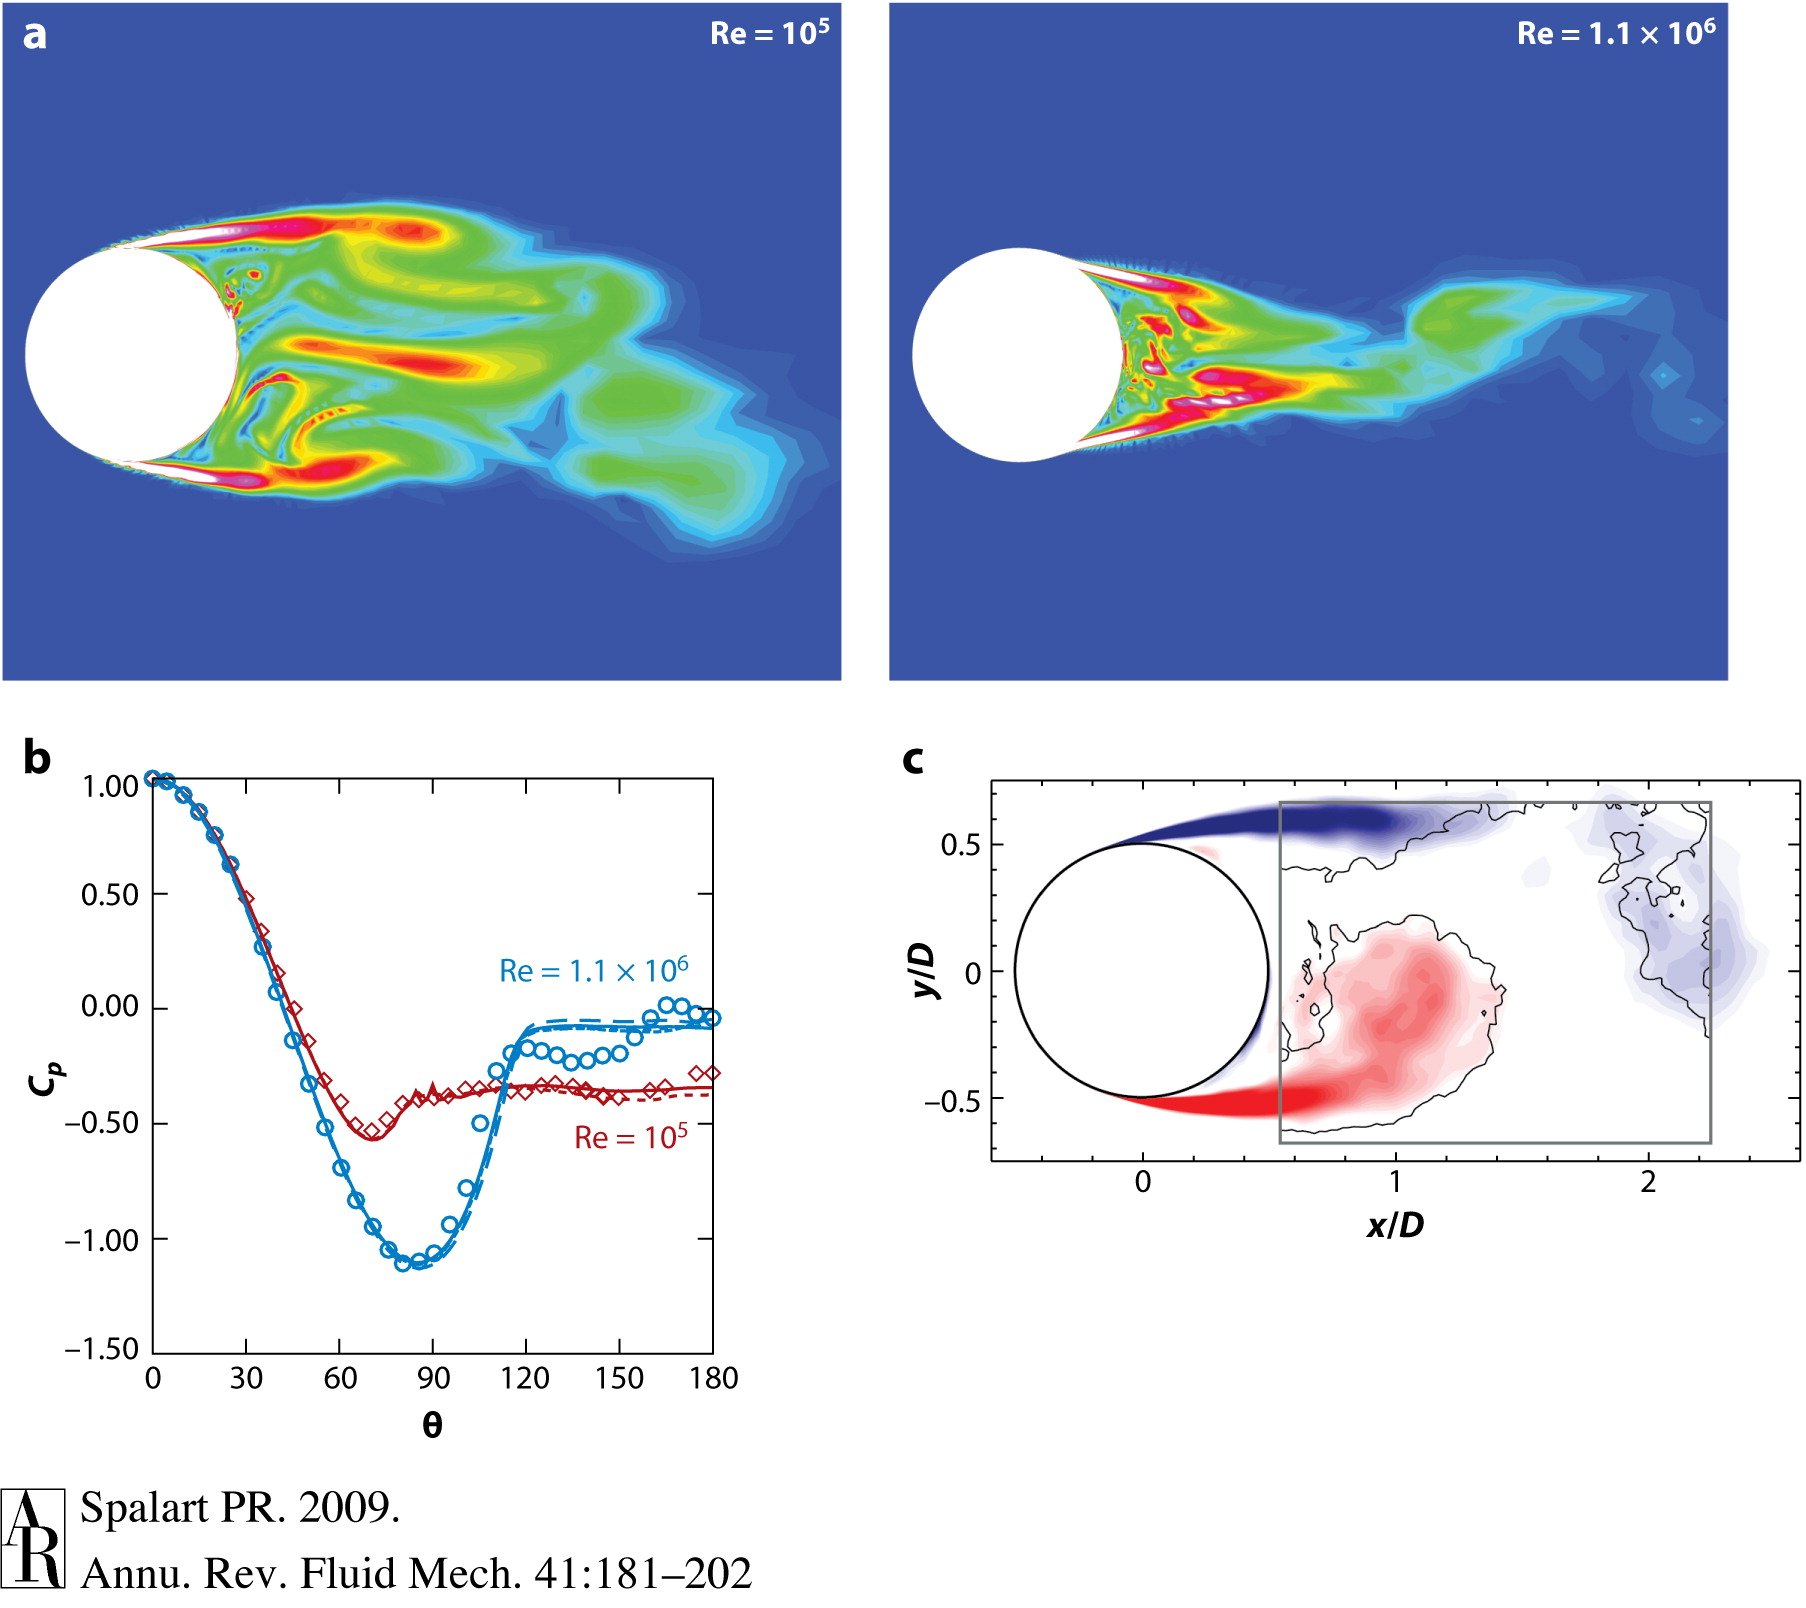
\includegraphics[width=0.8\textwidth]{Images/logan/spalart2009detachededdy_SphereSeparation.jpeg}
\caption{ DES results of velocity contours for flow over spheres from \cite{spalart2009detachededdy}. Simulation surface pressure distribution (solid line) compared to experiment (open marker) from \cite{squires2004detachededdy}.  Vorticity contours from simulation and experiment (outline) from \cite{mockett2008demonstration} }
\label{fig:desspherevalidation}
\end{center}
\end{figure}
%%\vspace{-2em}








Hybrid RANS/LES techniques have also demonstrated maturity for highly complex bluff-body geometries. Fig~\ref{fig:f15des} shows DES simulation vorticity isocontours for the complete geometry of an F-15 aircraft at high angle of attack $\alpha=65^o$, high Reynolds number $Re=13.6\times10^6$, and for a relatively incompressible wake at $M_{\infty}=0.3$ \cite{forsythe2004detachededdy}. In this study, DES simulation results were compared to Boeing’s stability and control database and similar RANS CFD simulations. It was found that the DES results agreed with the database more favorably than RANS for time-averaged load results such as lift and drag. However, both methods of simulation were within 10\% of the database and DES was shown to be seven times more expensive than RANS, so this is another an example of a situation where engineering judgment would be necessary to determine the most appropriate and efficient technique to use for the specific application. DES might prove advantageous in providing more accurate data for building an empirical model but RANS might be a more feasible tool for building an extensive CFD database for this fighter aircraft.

%%% F15 DES
%%\vspace{-2em}
% \begin{figure}[htb]
\begin{figure}[H]
\begin{center}
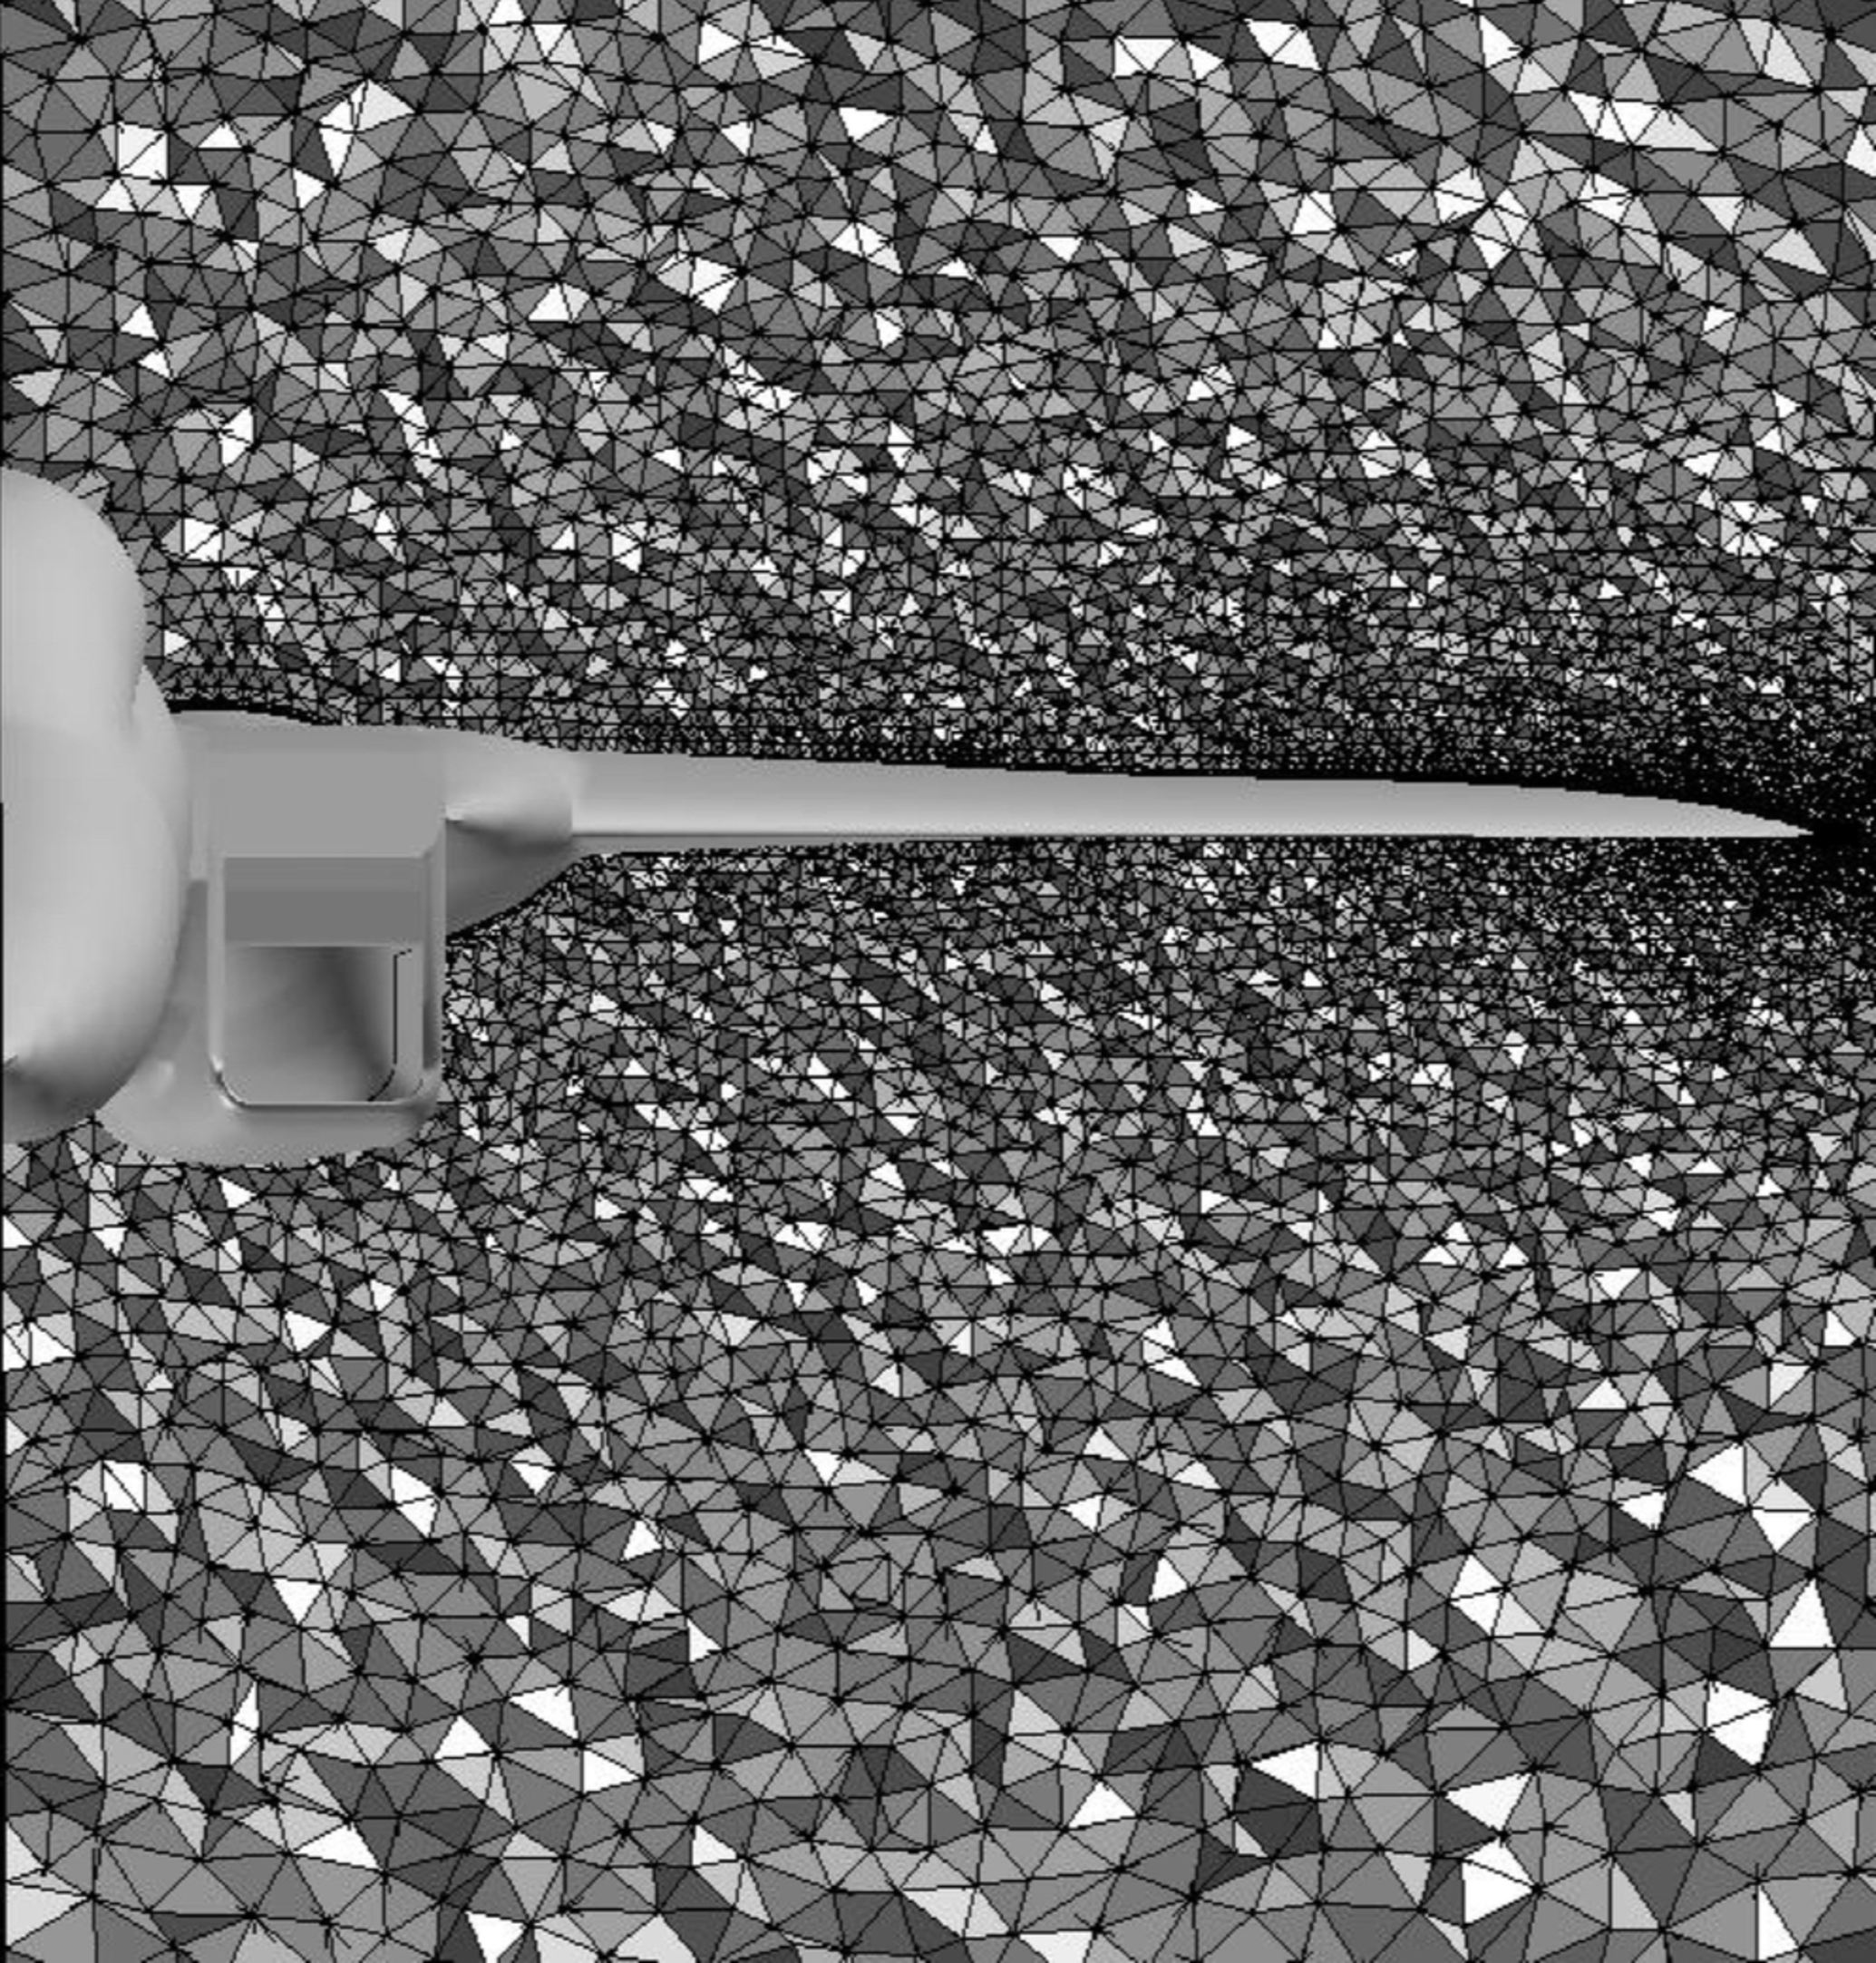
\includegraphics[width=0.45\textwidth]{Images/logan/forsythe2004detachededdy_f15grid.pdf}
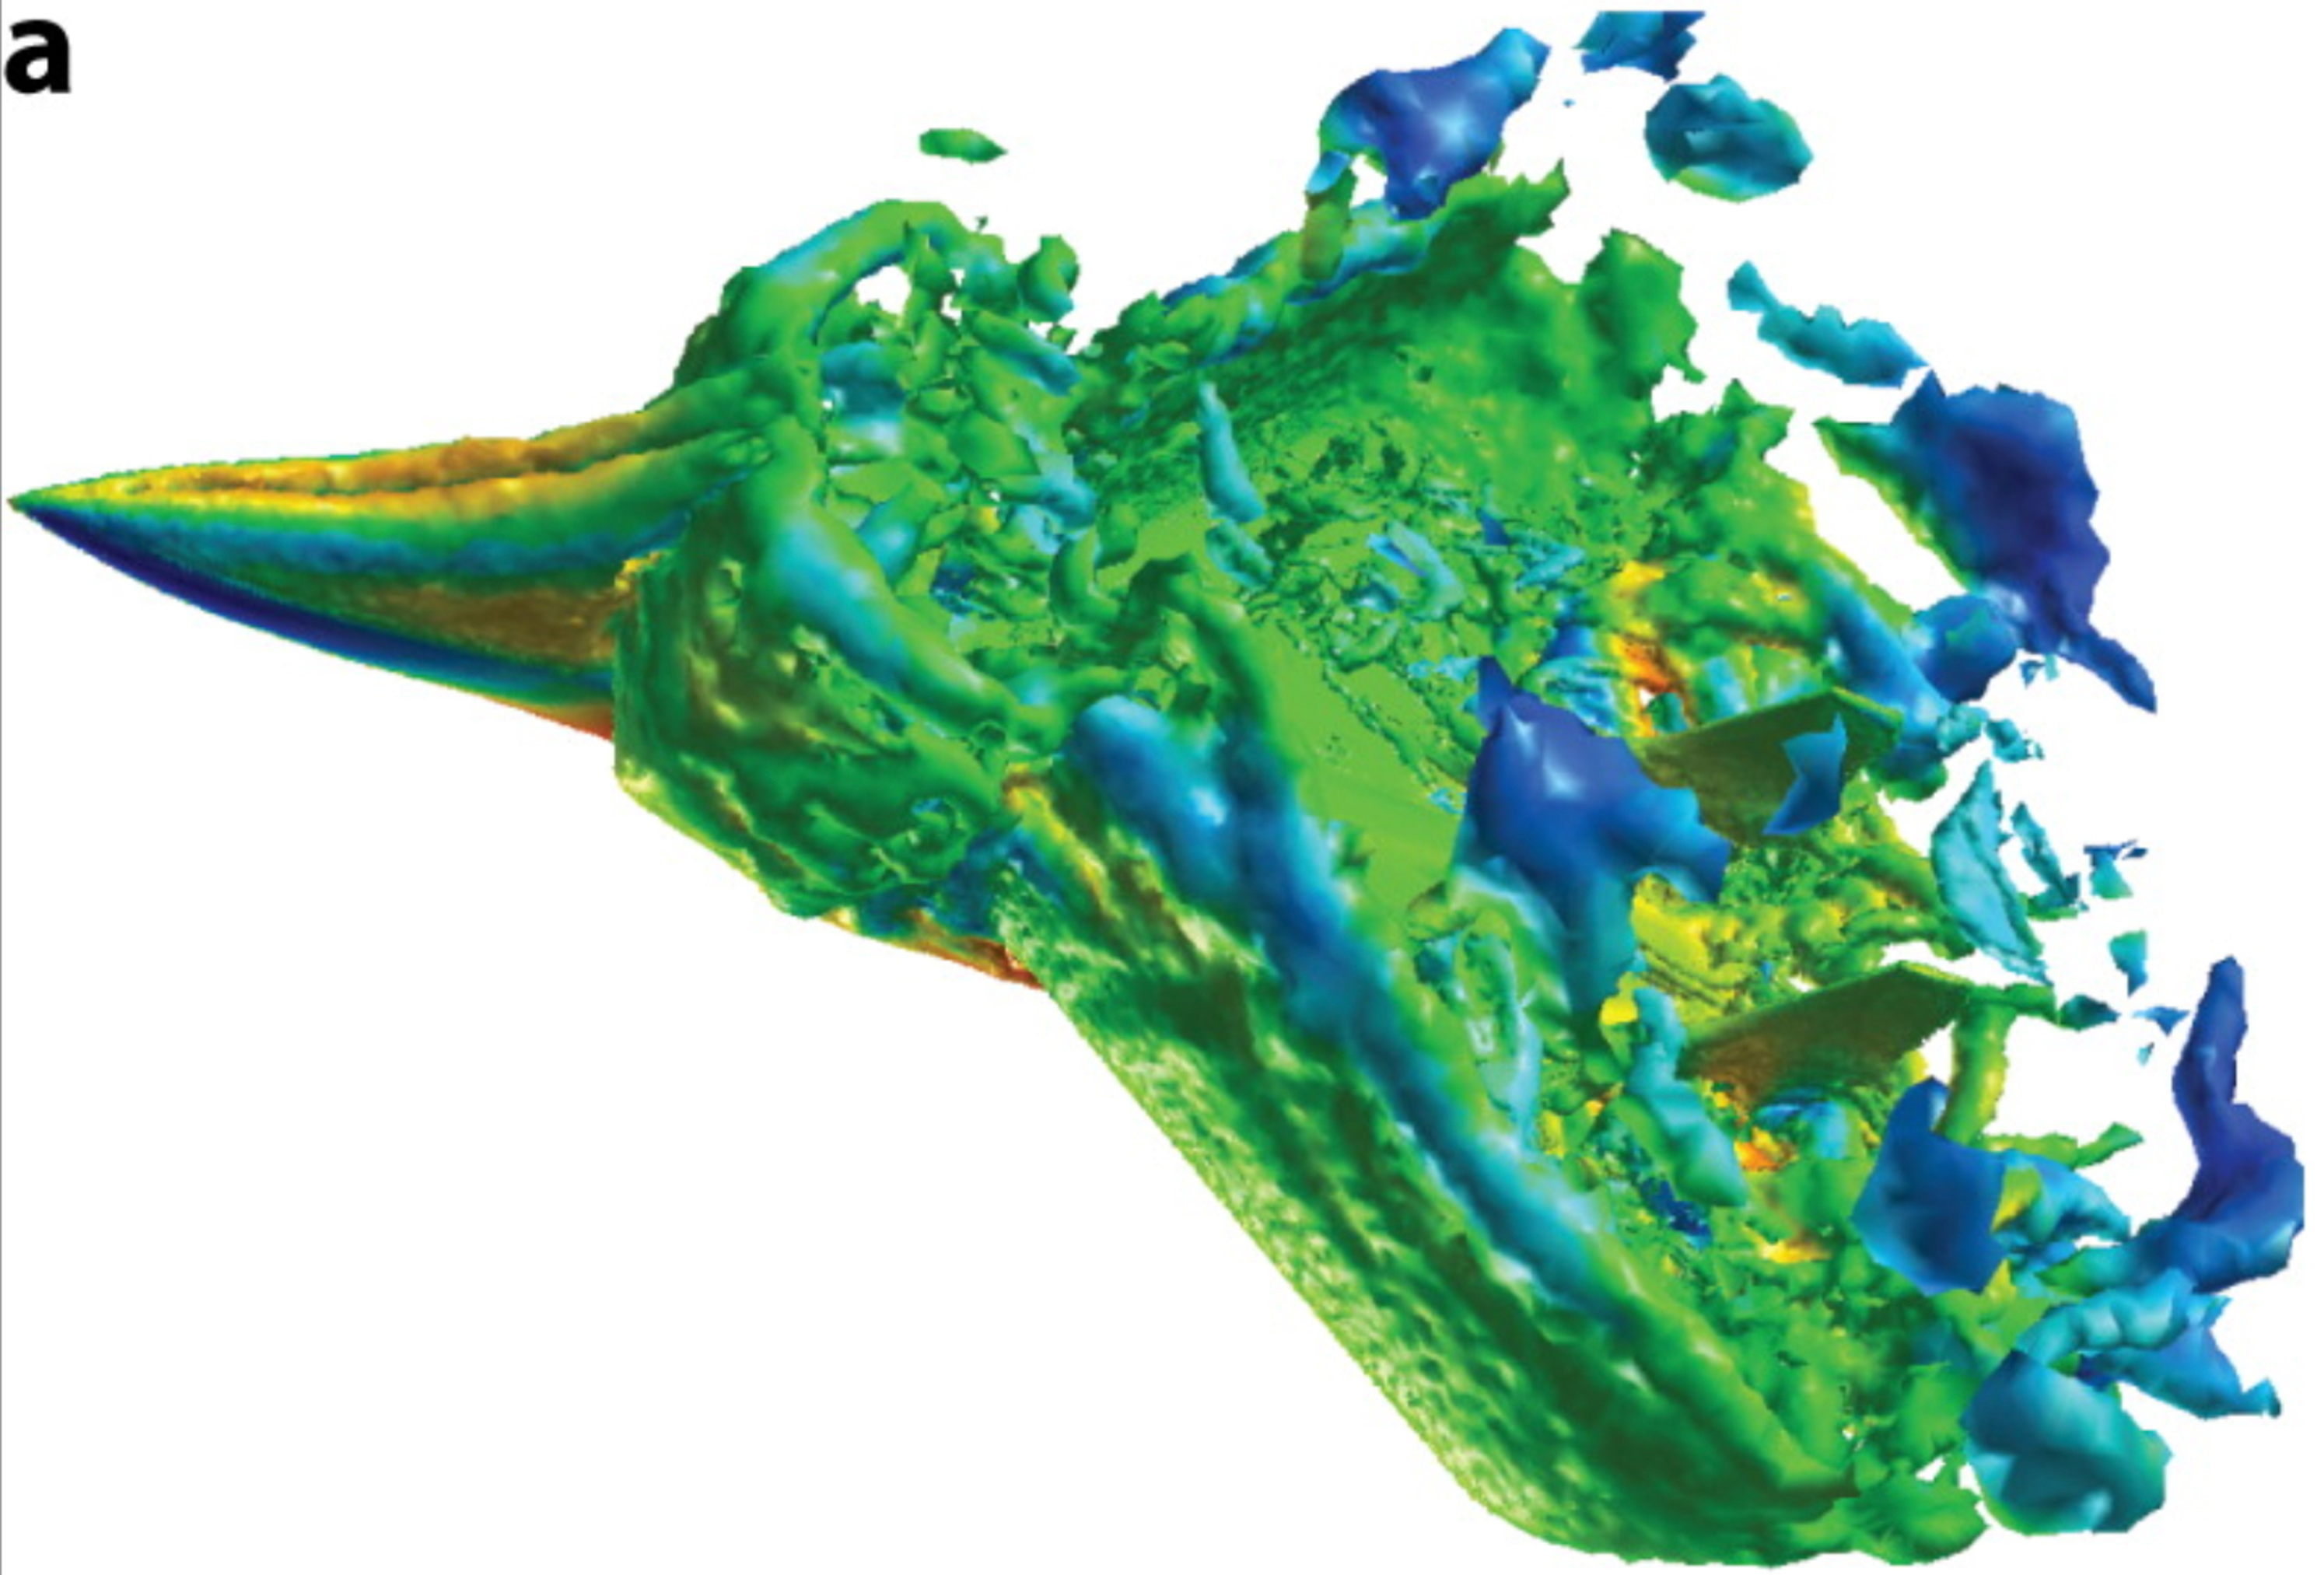
\includegraphics[width=0.45\textwidth]{Images/logan/spalart2009detachededdy_f15des.pdf}
\caption{ F-15 DES grid (left) \cite{forsythe2004detachededdy} vorticity isocontours (right) at $\alpha=65^o, \; Re_c=13.6\times10^6, \; M_{\infty}=0.3$ \cite{spalart2009detachededdy} }
\label{fig:f15des}
\end{center}
\end{figure}
%%\vspace{-2em}





DES methods have also been shown to be effective in multi-disciplinary applications such as Computational Aeroacoustics (CAA), which combines CFD and Computational Acoustics (CA) in order to simulate the acoustic effects of aerodynamic flows \cite{mendonca2002towards}. Acoustic effects occur on a wide range of scales and are very closely related to the turbulence in a flow, so for this reason, it is advantageous to resolve turbulent structures directly with LES-like methods such as DES rather than relying on the often incorrect estimation of RANS turbulence models. The study by Mendonca et al. (2002) demonstrates the effectiveness of DES coupled with CA methods in noise prediction for a representative passenger vehicle, as shown in Fig~\ref{fig:cardes}. Acoustic signature results computed from LES and DES data were compared to experiment, and DES-based predictions were shown to be superior as they were run on higher-fidelity grids due to the lower computational demand of DES. This example again highlights the importance of computational efficiency, as LES was shown to be more realistic than DES by this study for an individual test case, but was infeasible to run at this level of fidelity for the actual application.






%%% CAR DES
%%\vspace{-2em}
% \begin{figure}[htb]
\begin{figure}[H]
\begin{center}
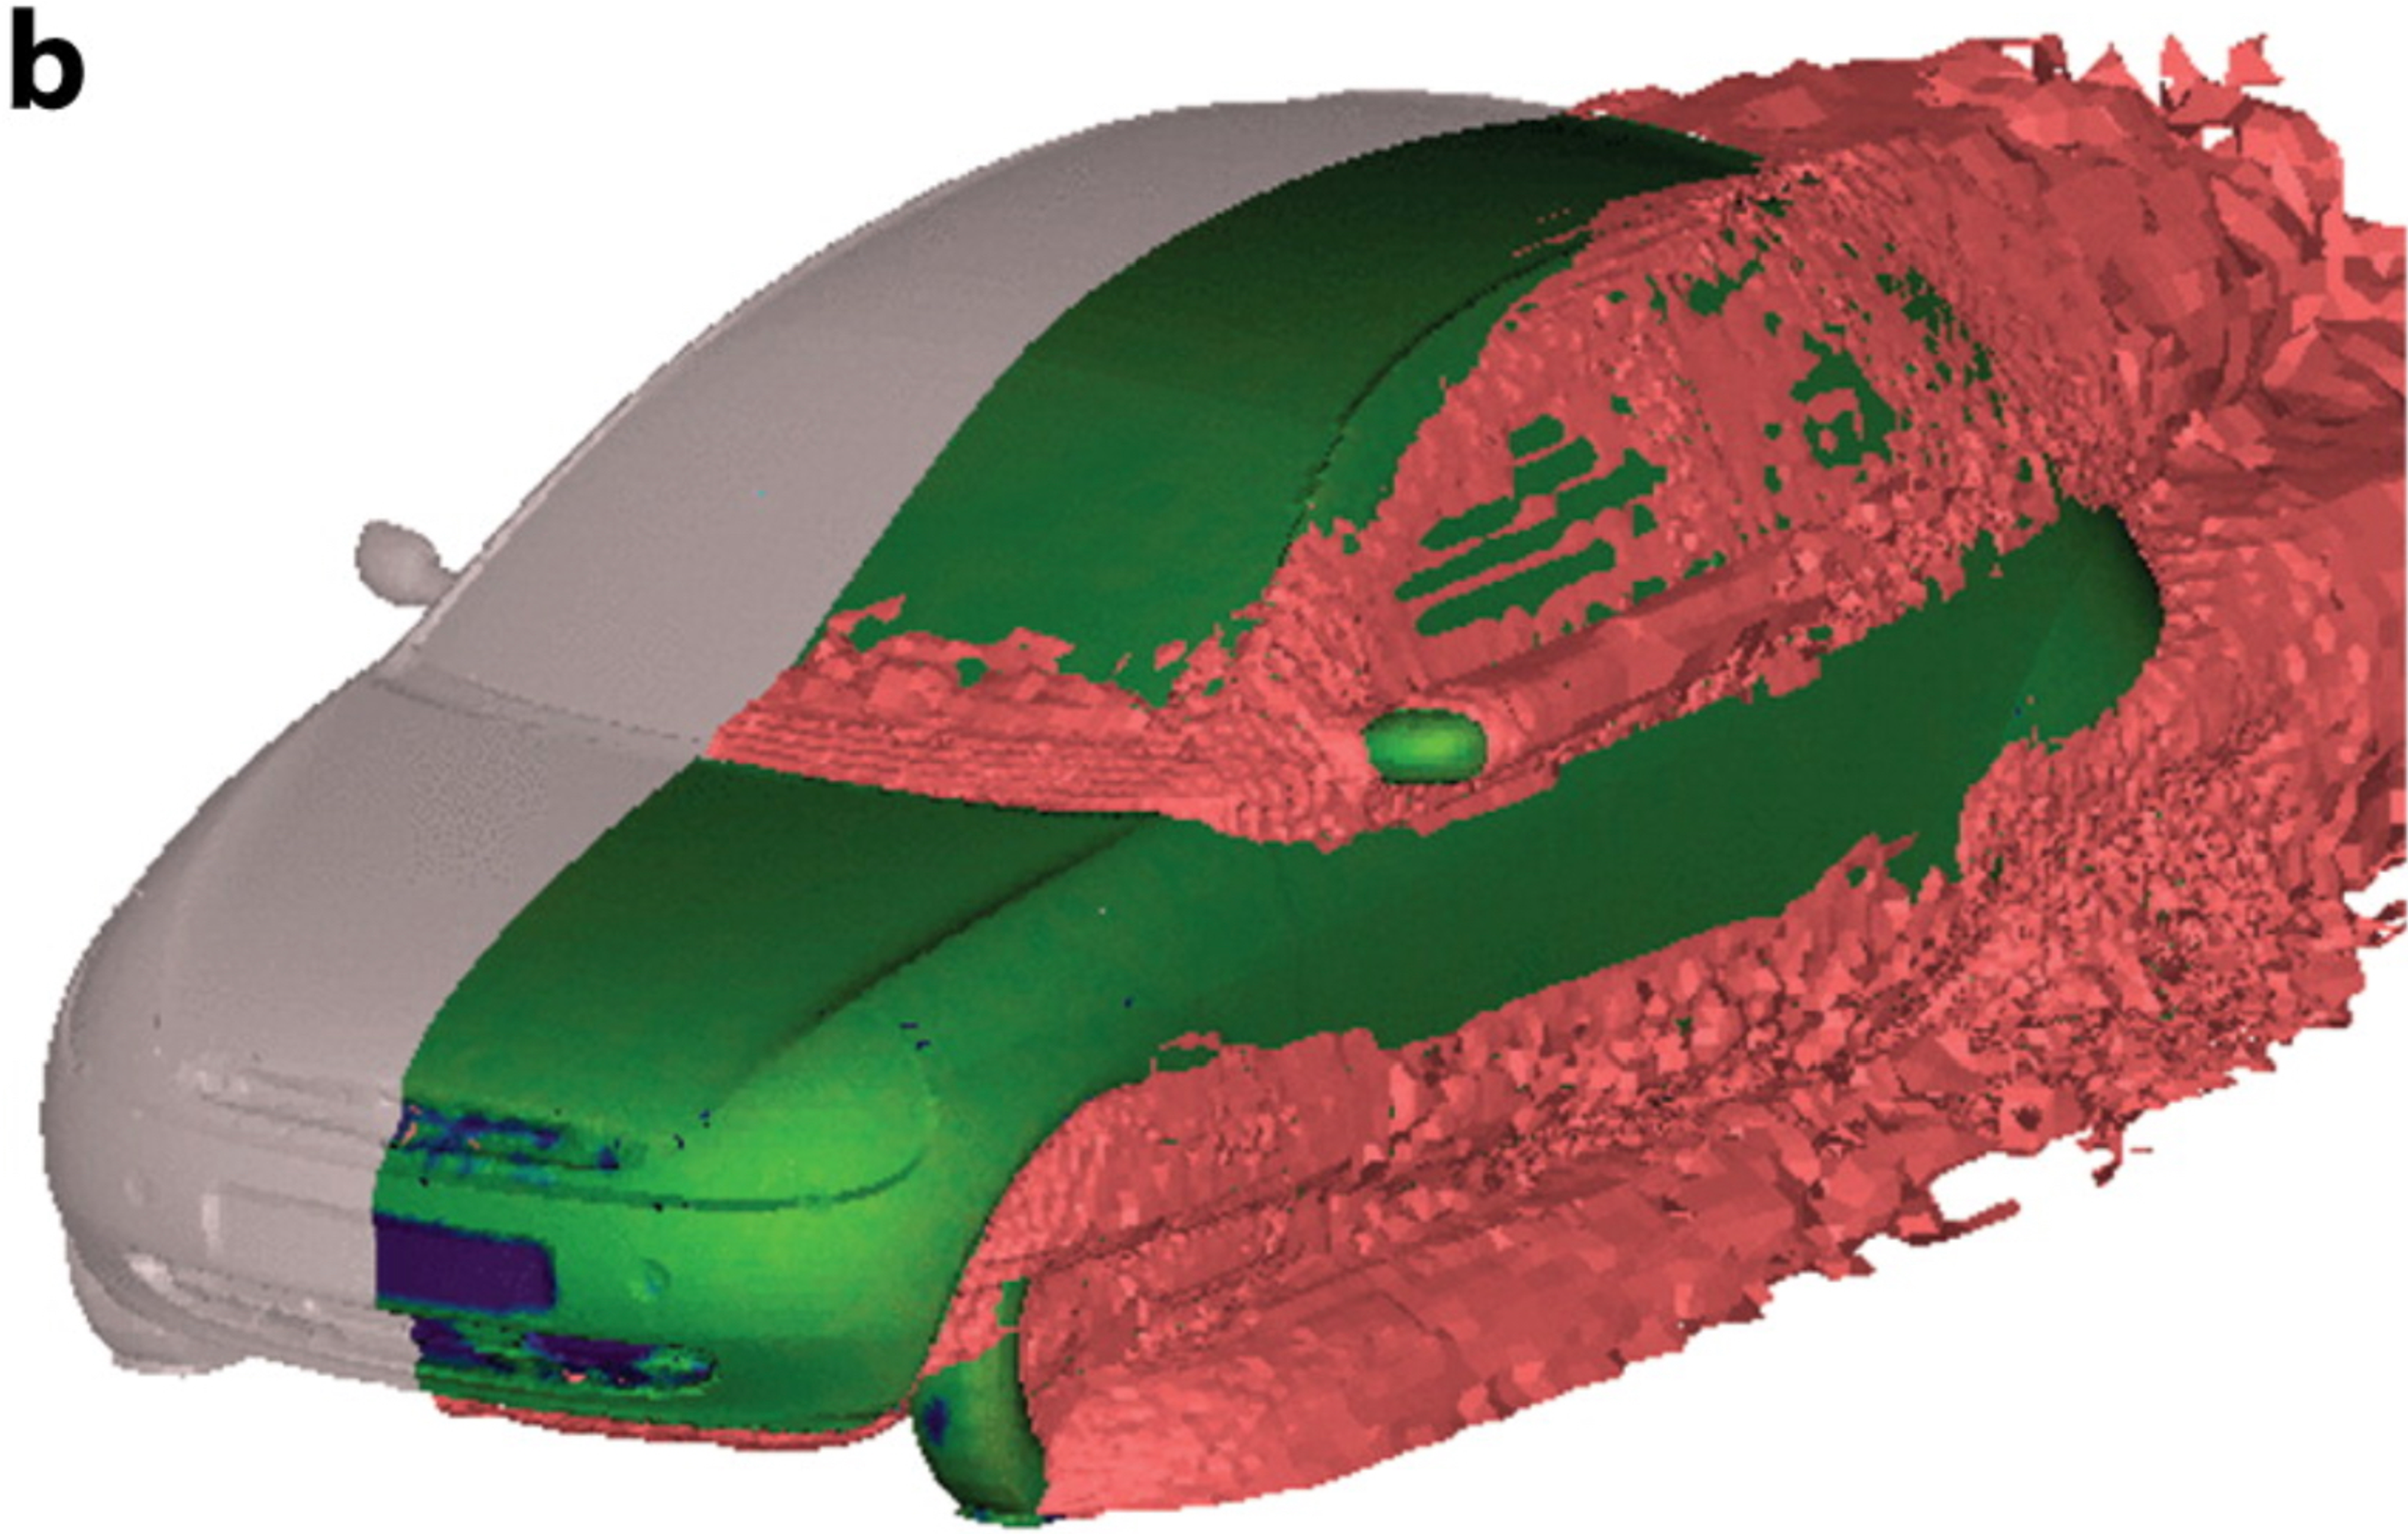
\includegraphics[width=0.5\textwidth]{Images/logan/spalart2009detachededdy_carDES.pdf}
\caption{ Acoustic source isocontours resulting from the DES-simulated flow over a representative passenger vehicle \cite{mendonca2002towards} }
\label{fig:cardes}
\end{center}
\end{figure}
%%\vspace{-2em}




Despite these successes, DES is not the all-in-one solution for computational modeling of massively separated flow over bluff-bodies. A number of deficiencies are inherent even in the fundamental nature of DES as a hybrid method. Rules for the hand-off between RANS and LES methods in the ``gray-area'' are approximate and potentially nonobjective. This can result in the RANS turbulence model ``contaminating'' the DNS results of the LES solution in the gray-area \cite{spalart2009detachededdy}. In situations where the grid near the surface is spaced such that LES is performed on an insufficiently fine grid, flow separation can occur at non-physical locations for simulations in which a pure-RANS model might predict the correct location of separation, as shown in Fig~\ref{fig:desgridinducedseparation}. Grid-based misbehavior of DES can be compensated for by using comparable methodologies like SAS or more advanced (and computationally expensive) formulations of DES like Delayed DES (DDES), which detects boundary layer regions and delays the switch from RANS to LES in order to preserve the turbulence modeling of the shear layer.

Thus, DES cannot be used as a simple ``plug-and-play'' turbulence model option (though it can be chosen from a turbulence model menu as such). A DES user must be aware of non-physical flow behavior and common geometry and grid features that may lead to these failures. Finally, DES may prove insufficient for some applications that require high orders of numeric accuracy to avoid numeric dissipation or resolve fine acoustic signals. In a DES solution where both RANS and LES modeling is present, it is extremely difficult to propose an order of accuracy of the composite solution. Even at a minimum, a lack of quantification of accuracy creates a deficiency in the ability to quality control a DES solution \cite{spalart2009detachededdy}.


%%% GRID INDUCED SEPARATION FROM DES
%%\vspace{-2em}
% \begin{figure}[htb]
\begin{figure}[H]
\begin{center}
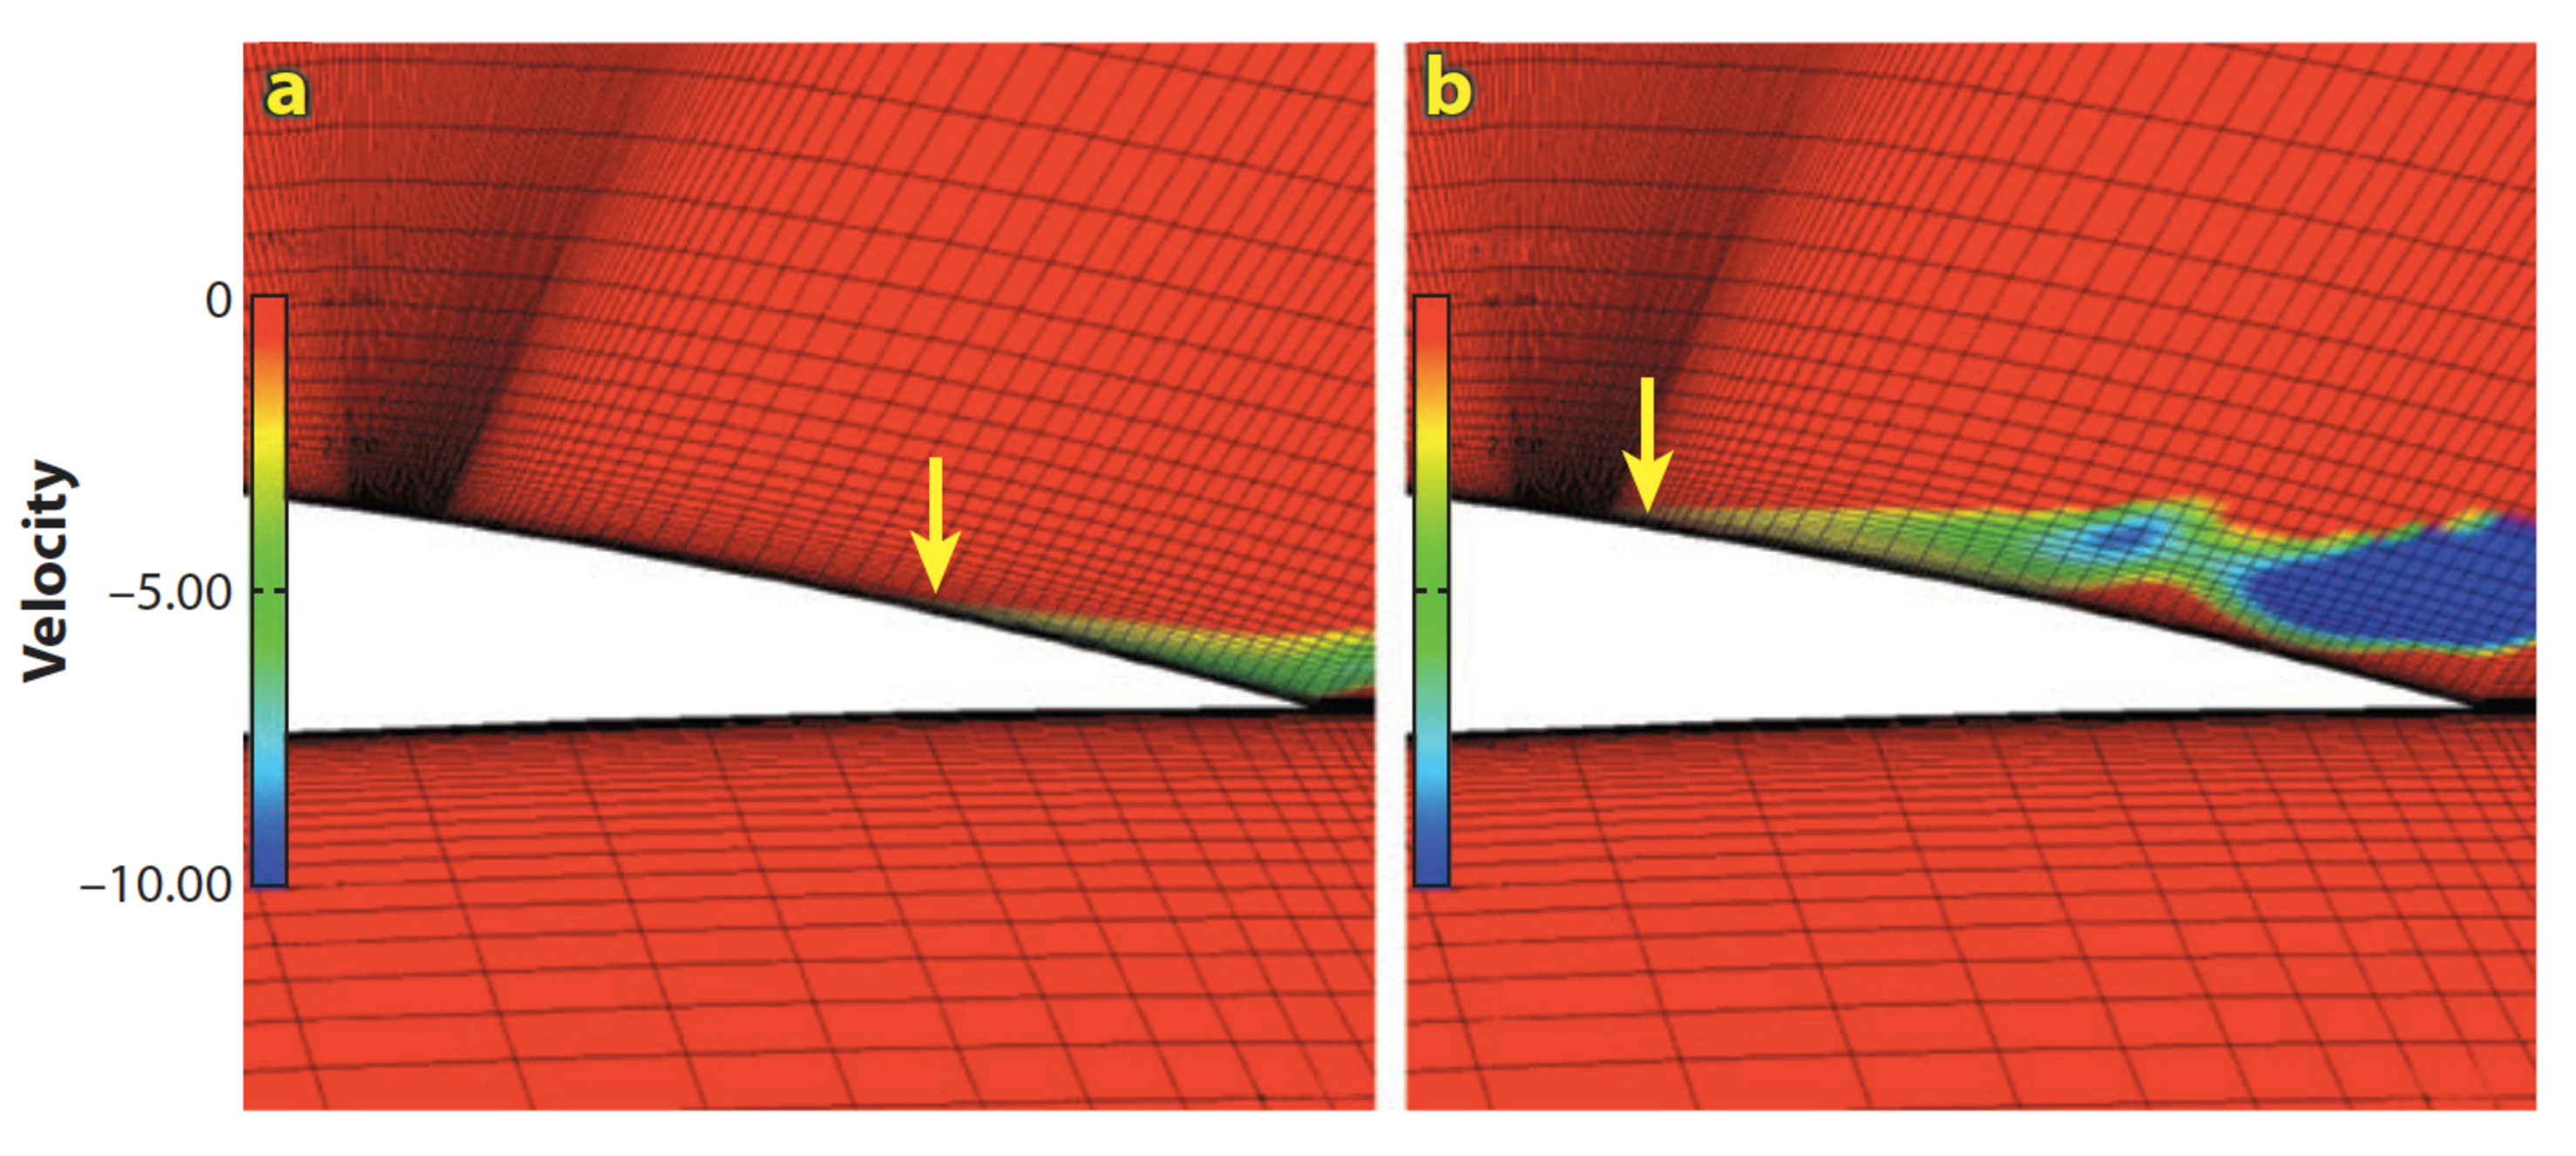
\includegraphics[width=0.6\textwidth]{Images/logan/spalart2009detachededdy_GridInducedSeparation.pdf}
\caption{ Vorticity contours over an airfoil for RANS (left) and DES (right) simulations showing an example of DES Grid Induced Separation (GIS) (indicated by arrow) from \cite{spalart2009detachededdy}, source: \cite{menter2004adaptation} }
\label{fig:desgridinducedseparation}
\end{center}
\end{figure}
%%\vspace{-2em}


In spite of its deficiencies, however, DES proves to be an extremely effective method for bluff-body simulations today, especially when compared to higher-order methods that alleviate the issues mentioned above. Non-hybrid LES methods offer improvements in accuracy and fidelity but come at a higher computational cost and with demand for more specialized grids and SGS modeling.

Even so, LES can still be thought of as a hybrid method of sorts, so an even more stark improvement in accuracy can be obtained by making the jump to full DNS: the ultimate end of the spectrum in high-fidelity CFD methodologies. In practice, however, this leap more often than not demands unattainable computational results. DNS results for flow over a sphere are presented in Fig~\ref{fig:dnssphere} from a study by Rodriguez et al. (2011) and compare well to experimental results \cite{rodriguez2011direct}. The only caveat is that these results are for a Reynolds number that is three orders of magnitude below that of the turbulent separation case achieved by DES in Fig~\ref{fig:desspherevalidation}. This low Reynolds number flow can prove useful as a testbed for other turbulence or empirical models, but is representative of only a small fraction of flow applications that can be found in the real-world.

%%% SPHERE DNS
%%\vspace{-2em}
% \begin{figure}[htb]
\begin{figure}[H]
\begin{center}
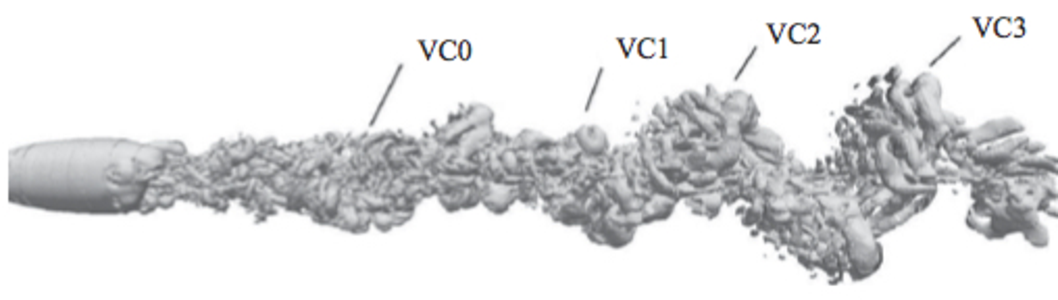
\includegraphics[width=0.45\textwidth]{Images/logan/rodriguez2011direct_DNSsphereWake.pdf}
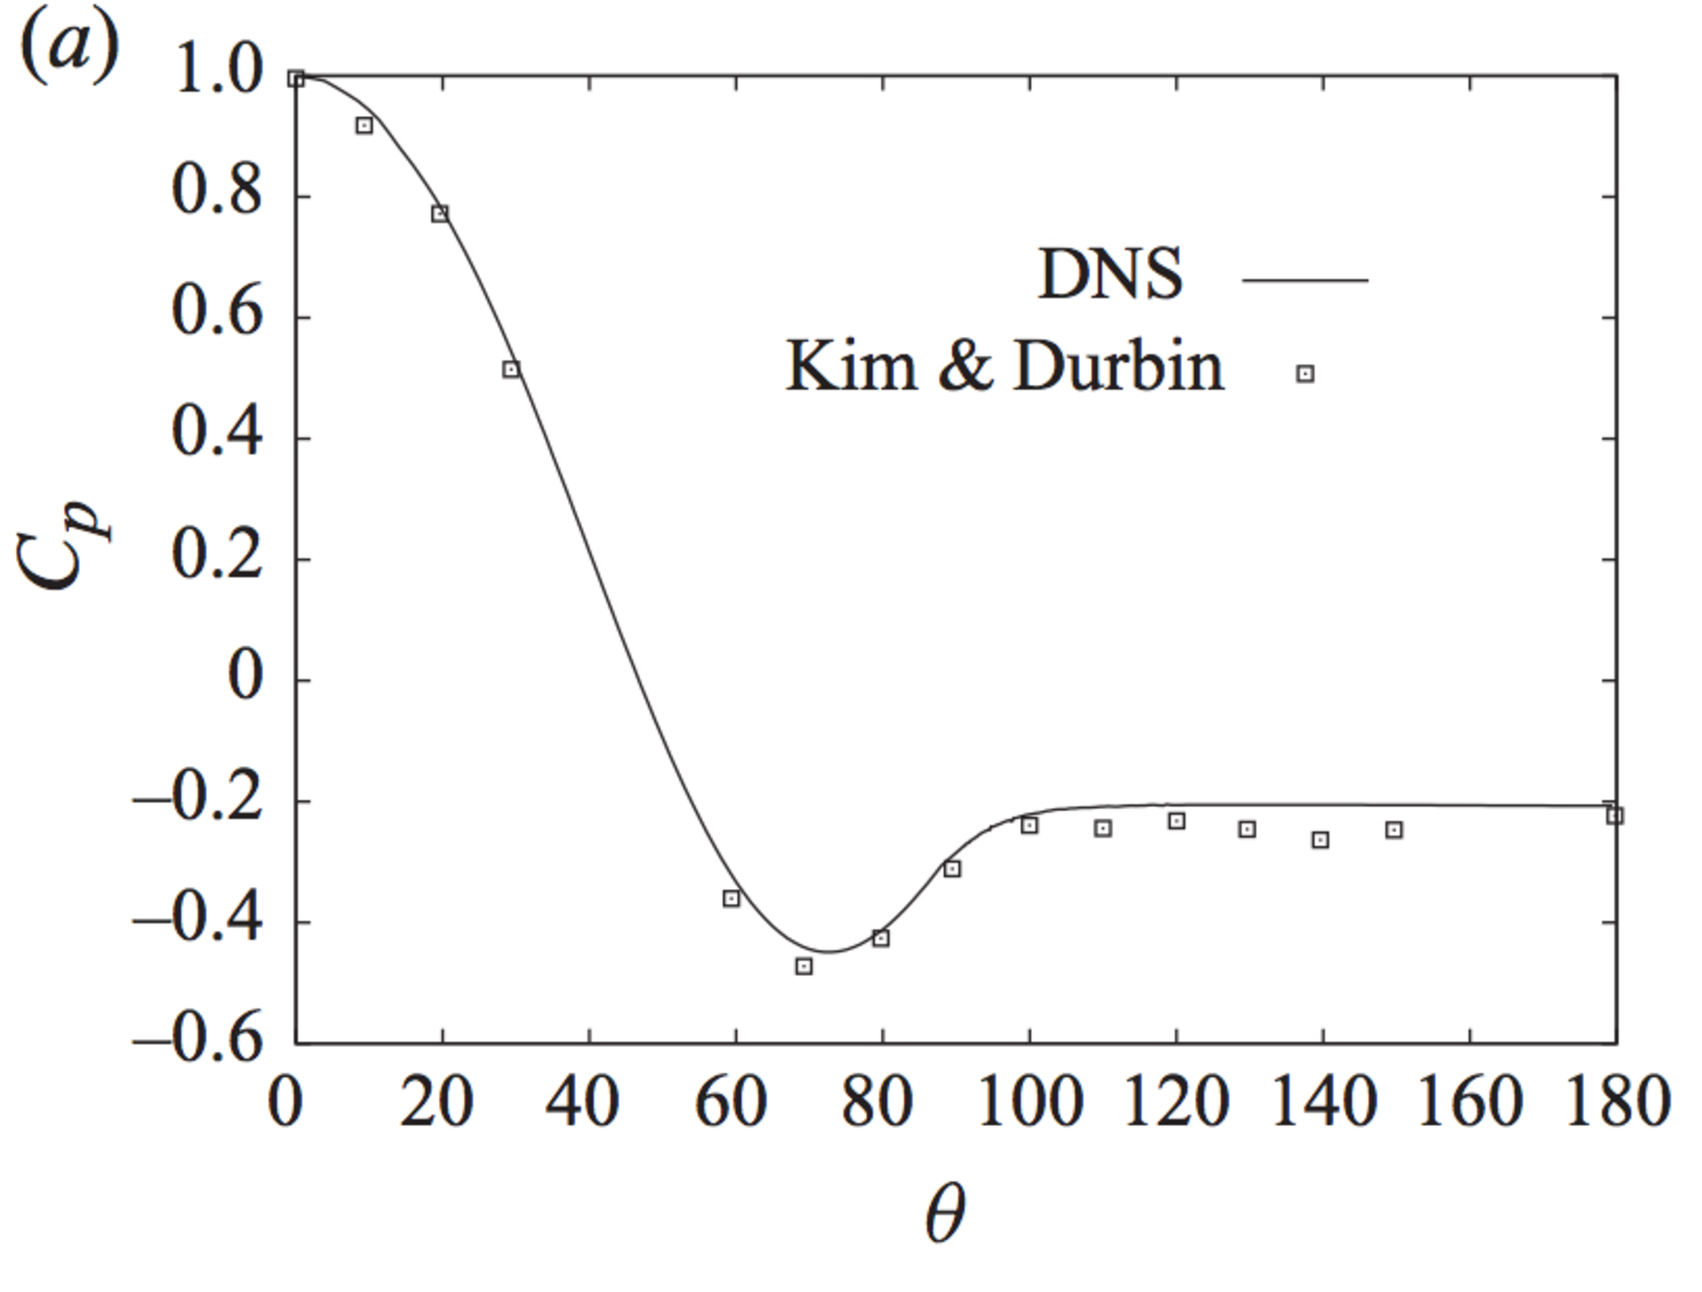
\includegraphics[width=0.45\textwidth]{Images/logan/rodriguez2011direct_DNSsphereCp.pdf}
\caption{ Instantaneous vortical structures (right) and mean surface pressure comparison (left) for DNS flow over a sphere ($Re_D = 3700$) \cite{rodriguez2011direct} }
\label{fig:dnssphere}
\end{center}
\end{figure}
%%\vspace{-2em}


DNS has been applied to more realistic bluff-body flows, such as the fabled dimpled golf ball, shown in Fig~\ref{fig:dnsgolfball} from Smith et al. (2010), and qualitative comparisons show that the results are reasonably realistic \cite{smith2010numerical}. From the figure, however, one can note the extreme fineness of the grid required to resolve DNS flow over a non-rotating golf ball at a Reynolds number still one order of magnitude below the DES example. Extrapolating this resolution of discretization to a complex case like the F-15 in Fig~\ref{fig:f15des} would be simply impossible to solve with today's computational technology.






%%% GOLF BALL DNS
%%\vspace{-2em}
% \begin{figure}[htb]
\begin{figure}[H]
\begin{center}
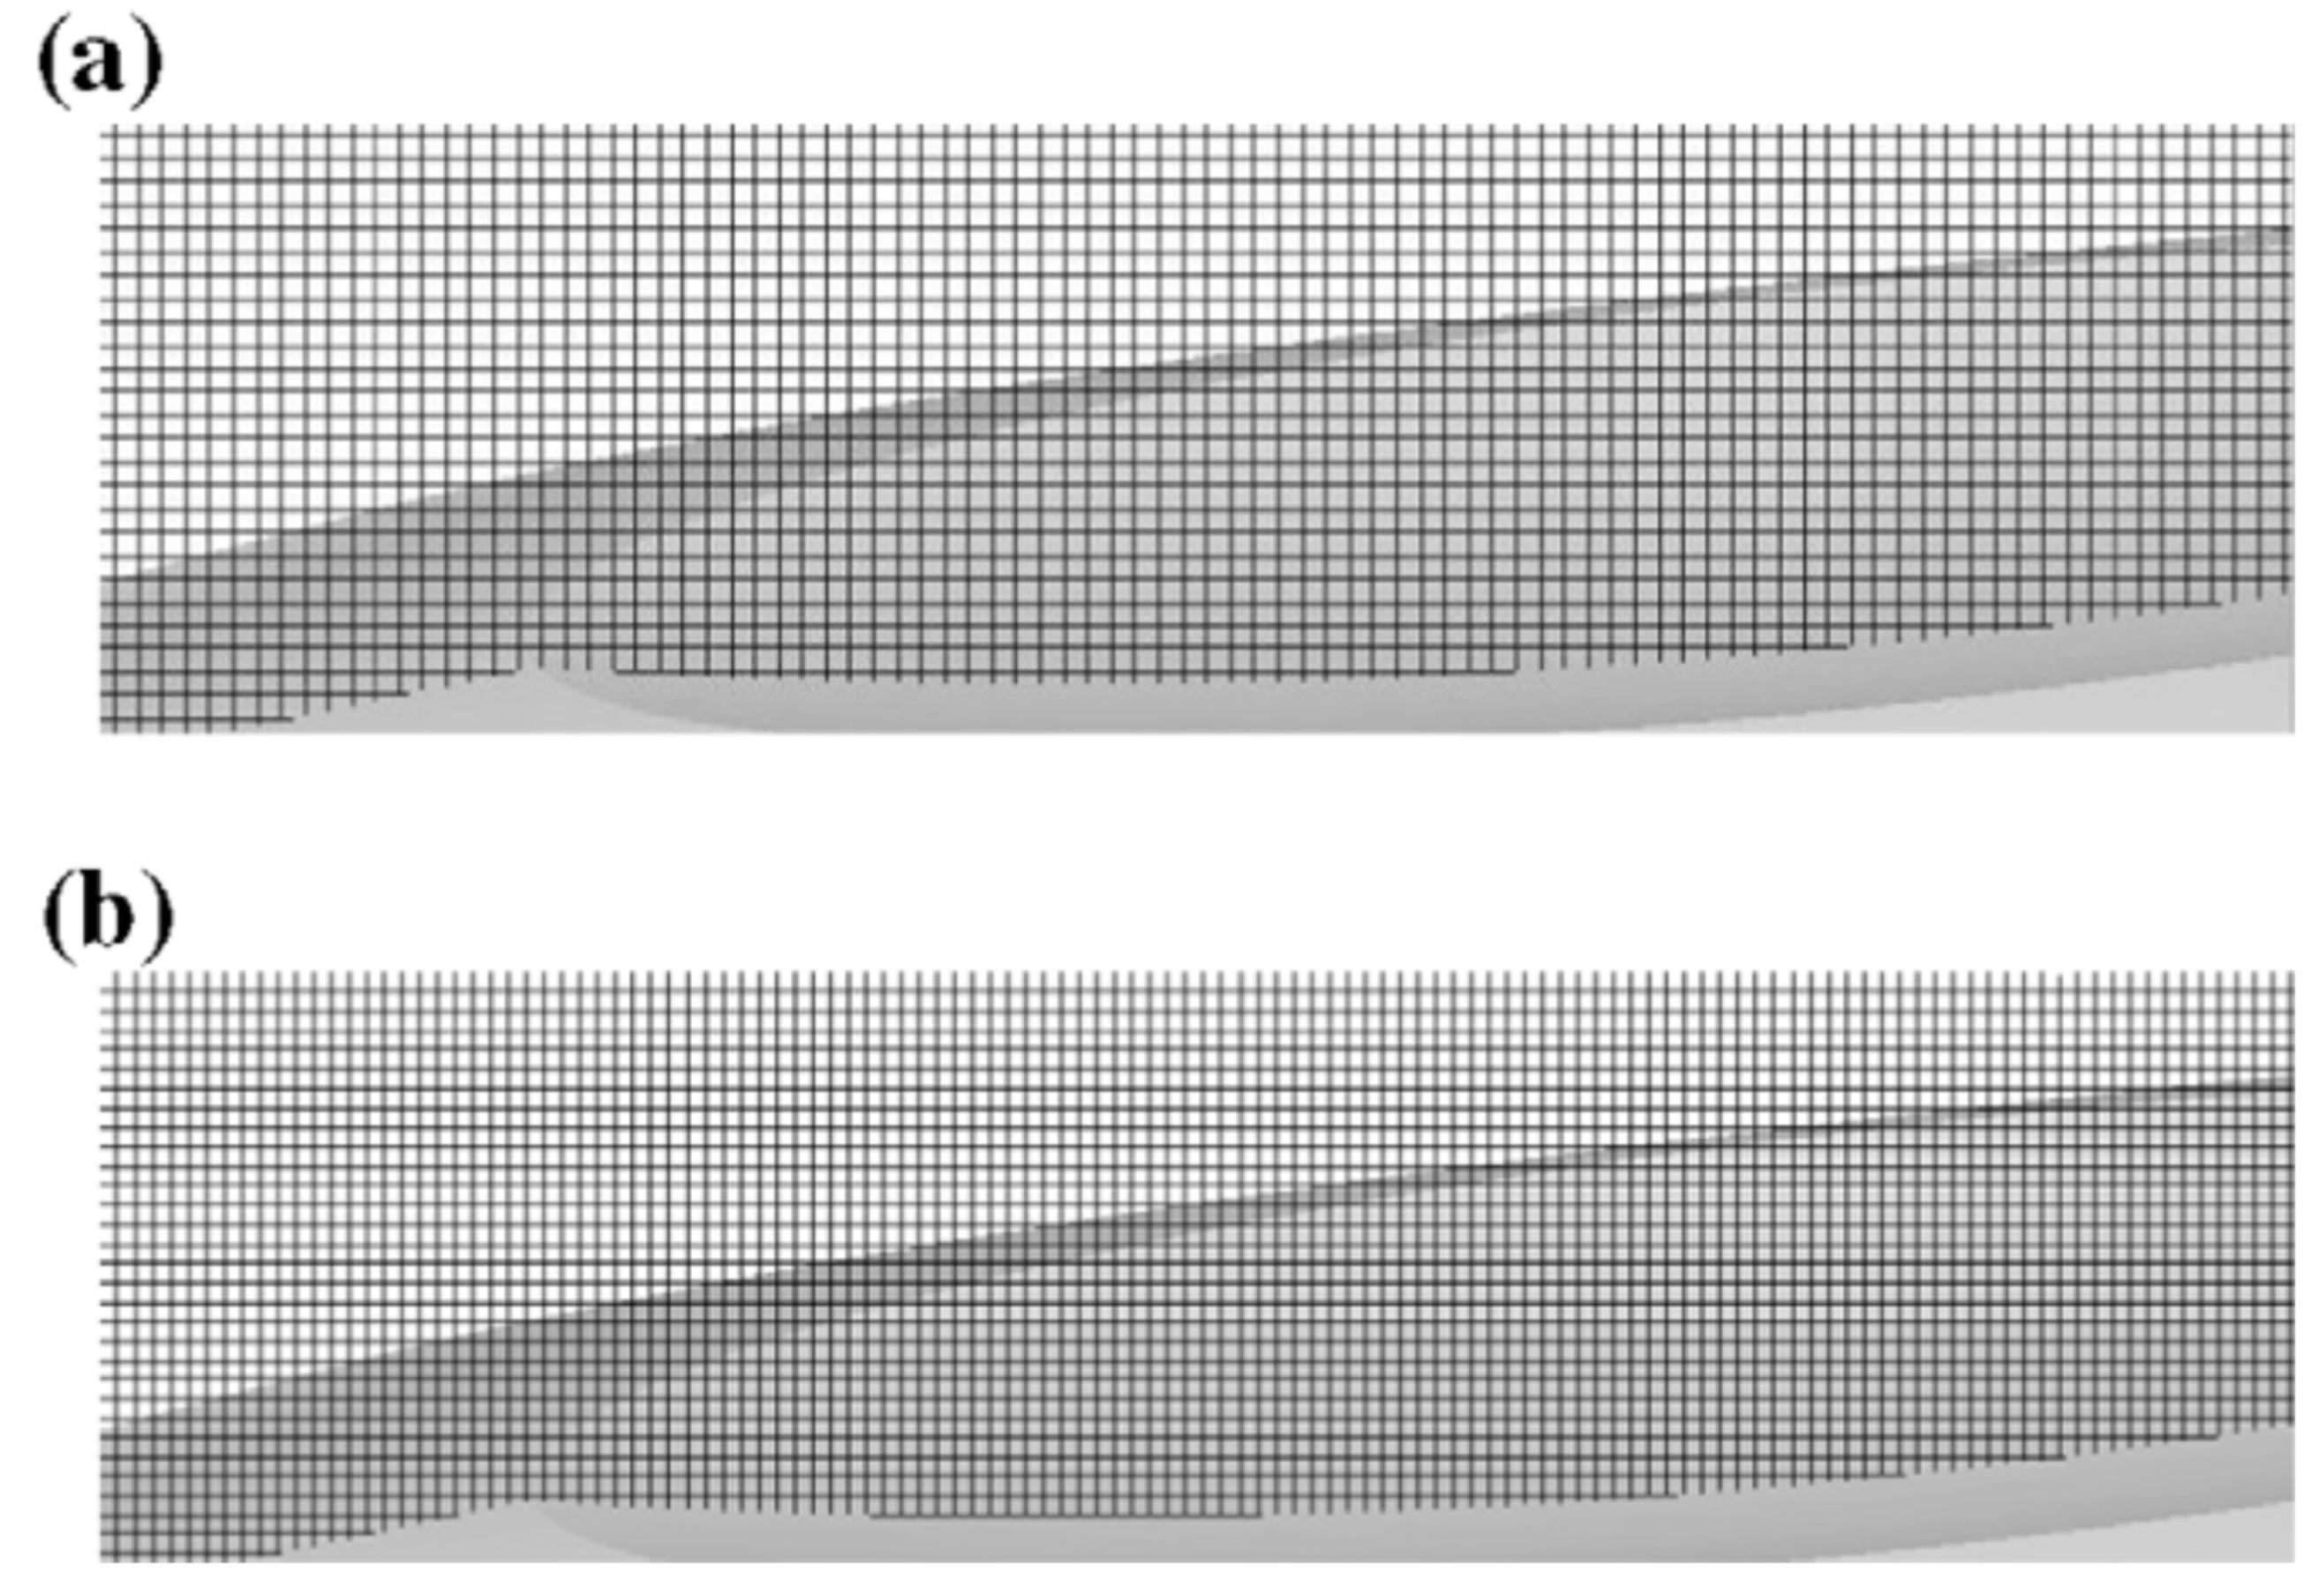
\includegraphics[width=0.40\textwidth]{Images/logan/smith2010numerical_golfballgrid.pdf}
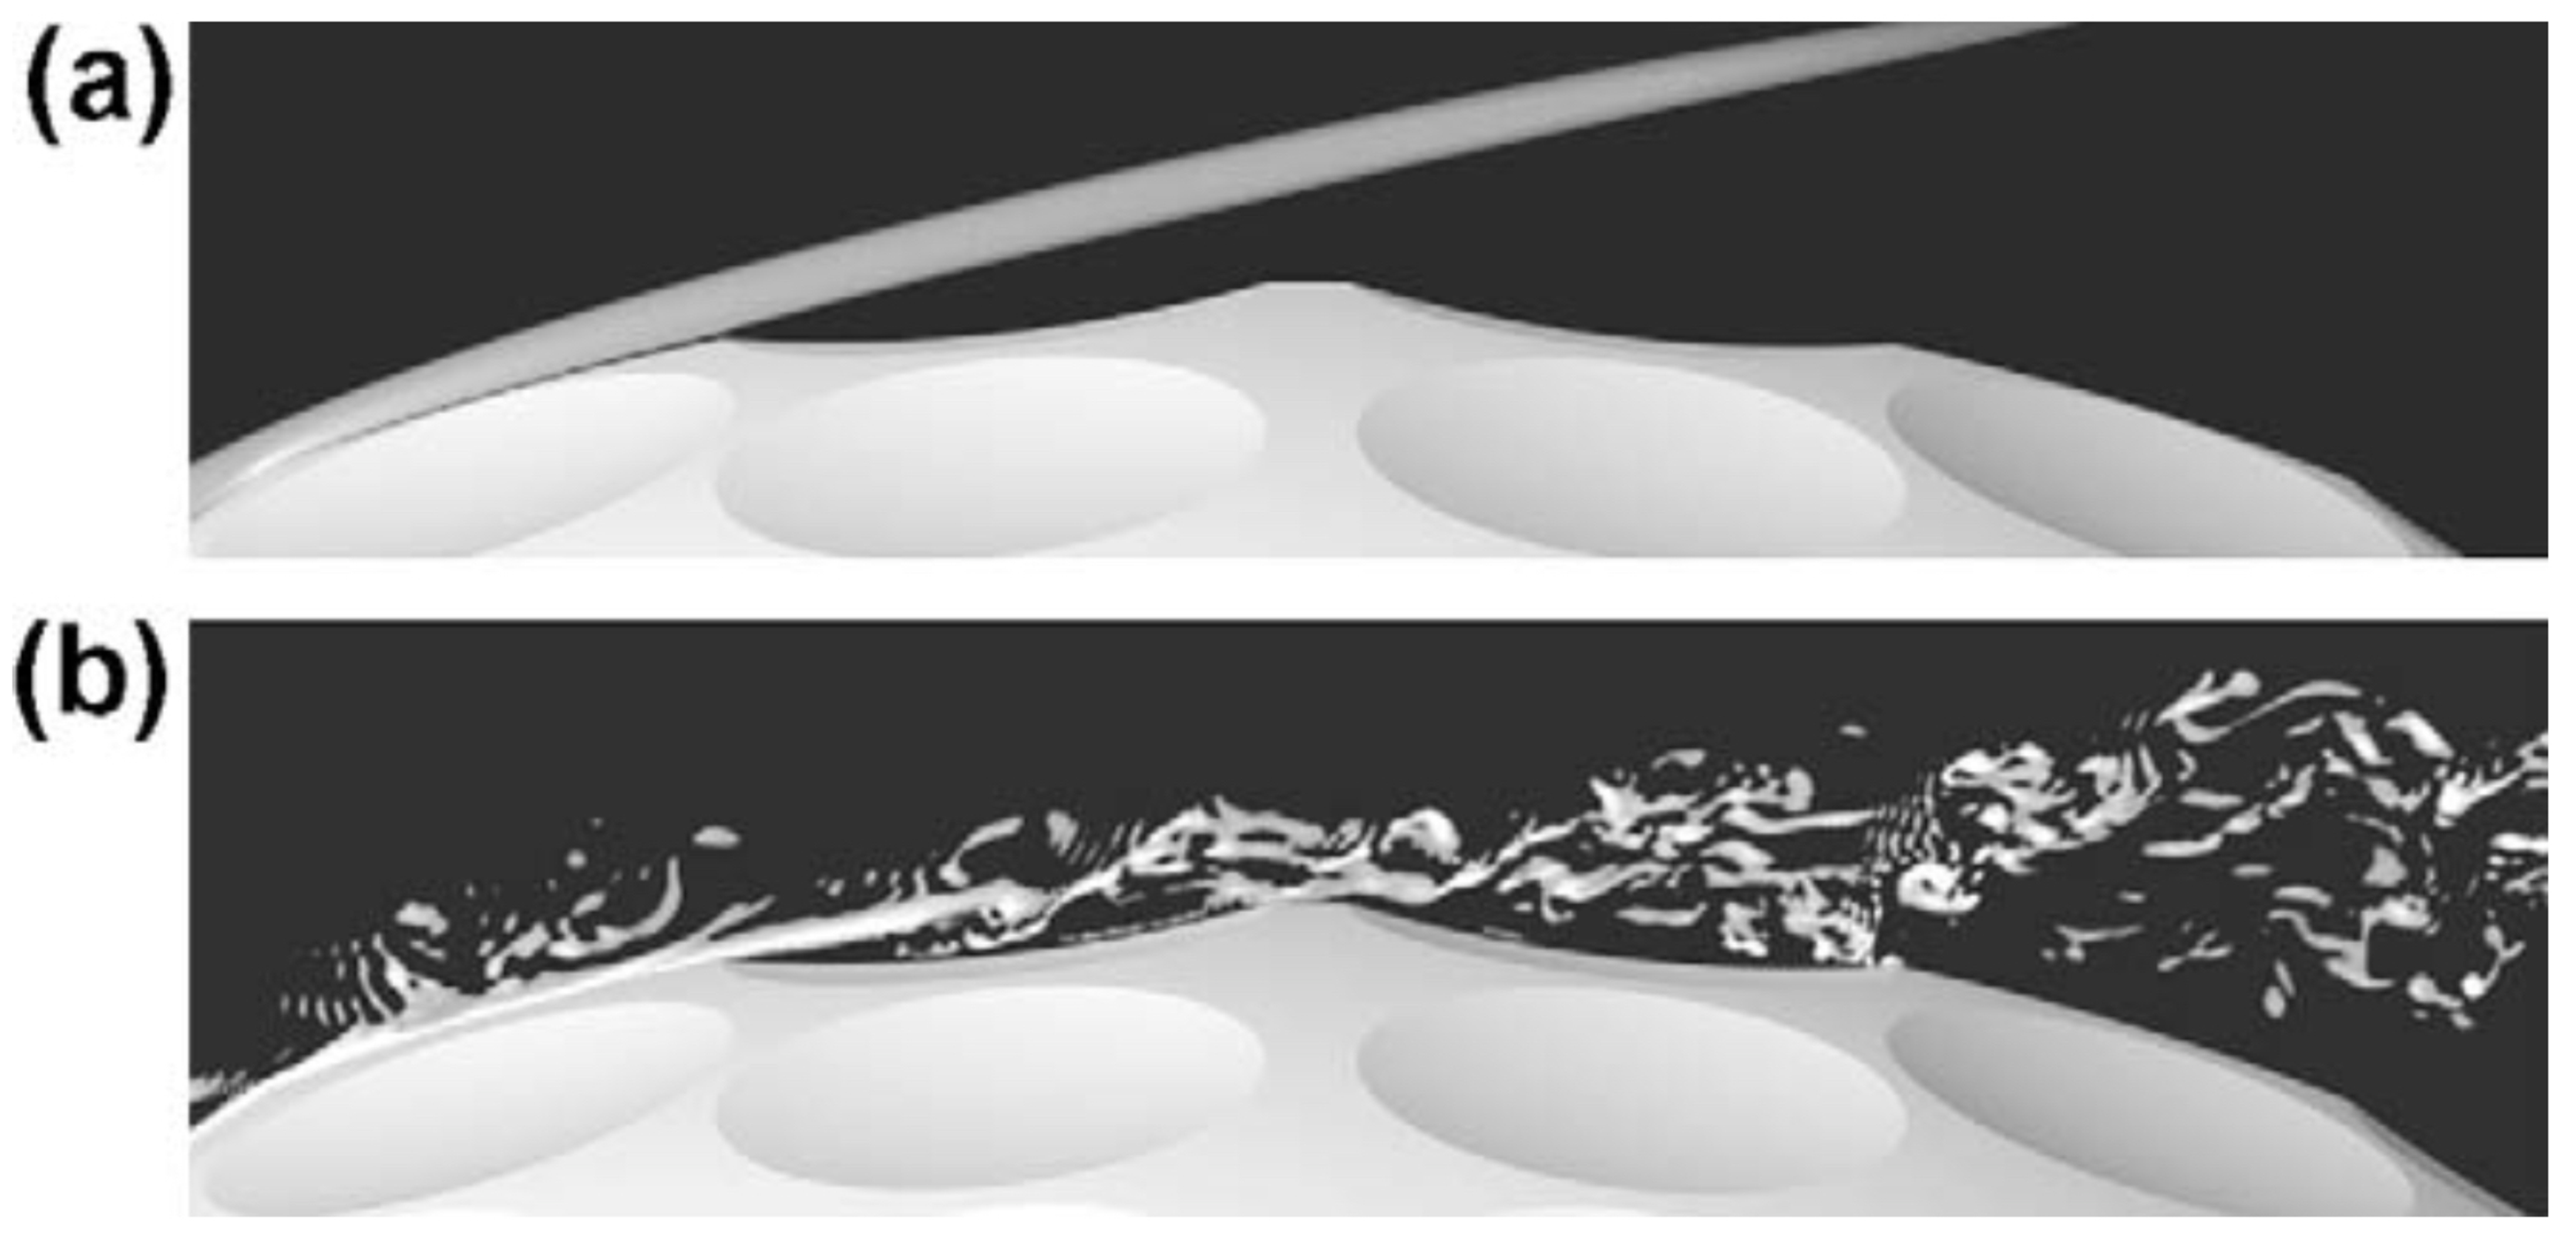
\includegraphics[width=0.55\textwidth]{Images/logan/smith2010numerical_golfballvorticity.pdf}
\caption{ DNS grid (left) and vorticity contours (right) for a non-rotating golf ball with dimples (a: $Re_D = 2.5\times10^4$, b: $Re_D=1.1\times10^5$) \cite{smith2010numerical} }
\label{fig:dnsgolfball}
\end{center}
\end{figure}
%%\vspace{-2em}















In summary, the current state-of-the-art in bluff-body flow simulation is a combination of CFD methodologies and greatly depends on the specific application. URANS simulations have been shown to match time-averaged loading and flow feature results of both experiment and more advanced computational methods under the correct geometry and flow conditions. A user aware of the limitations of URANS should be able to use this method in the appropriate applications as an extremely cost-saving alternative to higher-fidelity methods.

Still, in situations where the fine turbulent features of the massively separated flow behind a bluff-body is impossible to model with RANS or when higher accuracy is required in resolving unsteady flow behavior, the hybrid RANS/LES methodology of DES is preferable as the most mature and feasible implementation of direct simulation. This method combines the robustness of RANS in the boundary layer with the accuracy of DNS for the large turbulent structures in a formulation efficient enough to run accurately for complex bluff-bodies on today's computers.

Though more user-friendly than LES, DES is far from automatic. Ambiguous behavior with respect to geometry and grid refinement requires the user to be well trained in the correct application of DES. Other methodologies including DDES and SAS exist to alleviate some of these shortcomings, but come at their own cost of computational expense or reduction in accuracy. Solver selection between DES and SAS is, again, a decision that must be made with engineering judgment.

% SPALART TABLE OF TURBULENCE MODEL READINESS
%%\vspace{-2em}
% \begin{figure}[htb]
\begin{figure}[H]
\begin{center}
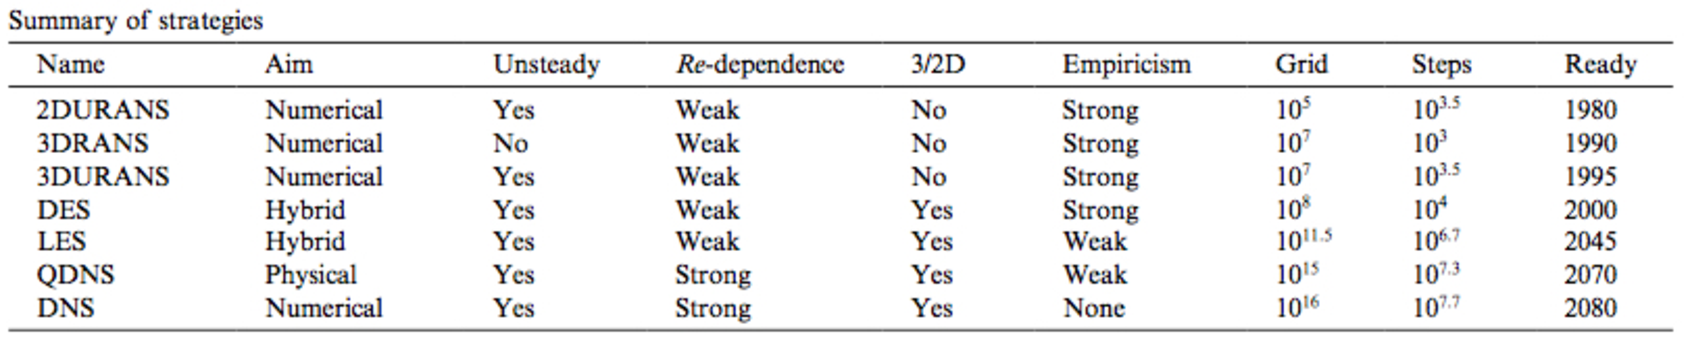
\includegraphics[width=0.95\textwidth]{Images/logan/spalart2000strategies_TurbModelTable.pdf}
\caption{ Spalart's review of turbulence model readiness (2000) \cite{spalart2000strategies} }
\label{fig:turbulencemodelreadiness}
\end{center}
\end{figure}
%%\vspace{-2em}

In the future, we can look forward to computational power improvements and LES methodology maturation. Artificial intelligence in grid refinement and solver selection may improve the hybridization of LES-like solutions, making them both more accurate and user-friendly \cite{spalart2000strategies}. DNS will continue to be important for RANS turbulence model calibration, but its true feasibility remains in the distant future, as roughly estimated by Spalart in Fig~\ref{fig:turbulencemodelreadiness} based on on the ``rule of thumb'' that computer power increases by a factor of five every five years. Based off of predictions like these, DNS is hardly a technology to wait on in today's industry, and RANS and DES will continue their reign, supplemented with experimental validation.






















% %%% LES VS RANS CYLINDER
% %%\vspace{-2em}
% % \begin{figure}[htb]
% \begin{figure}[H]
% \begin{center}
% 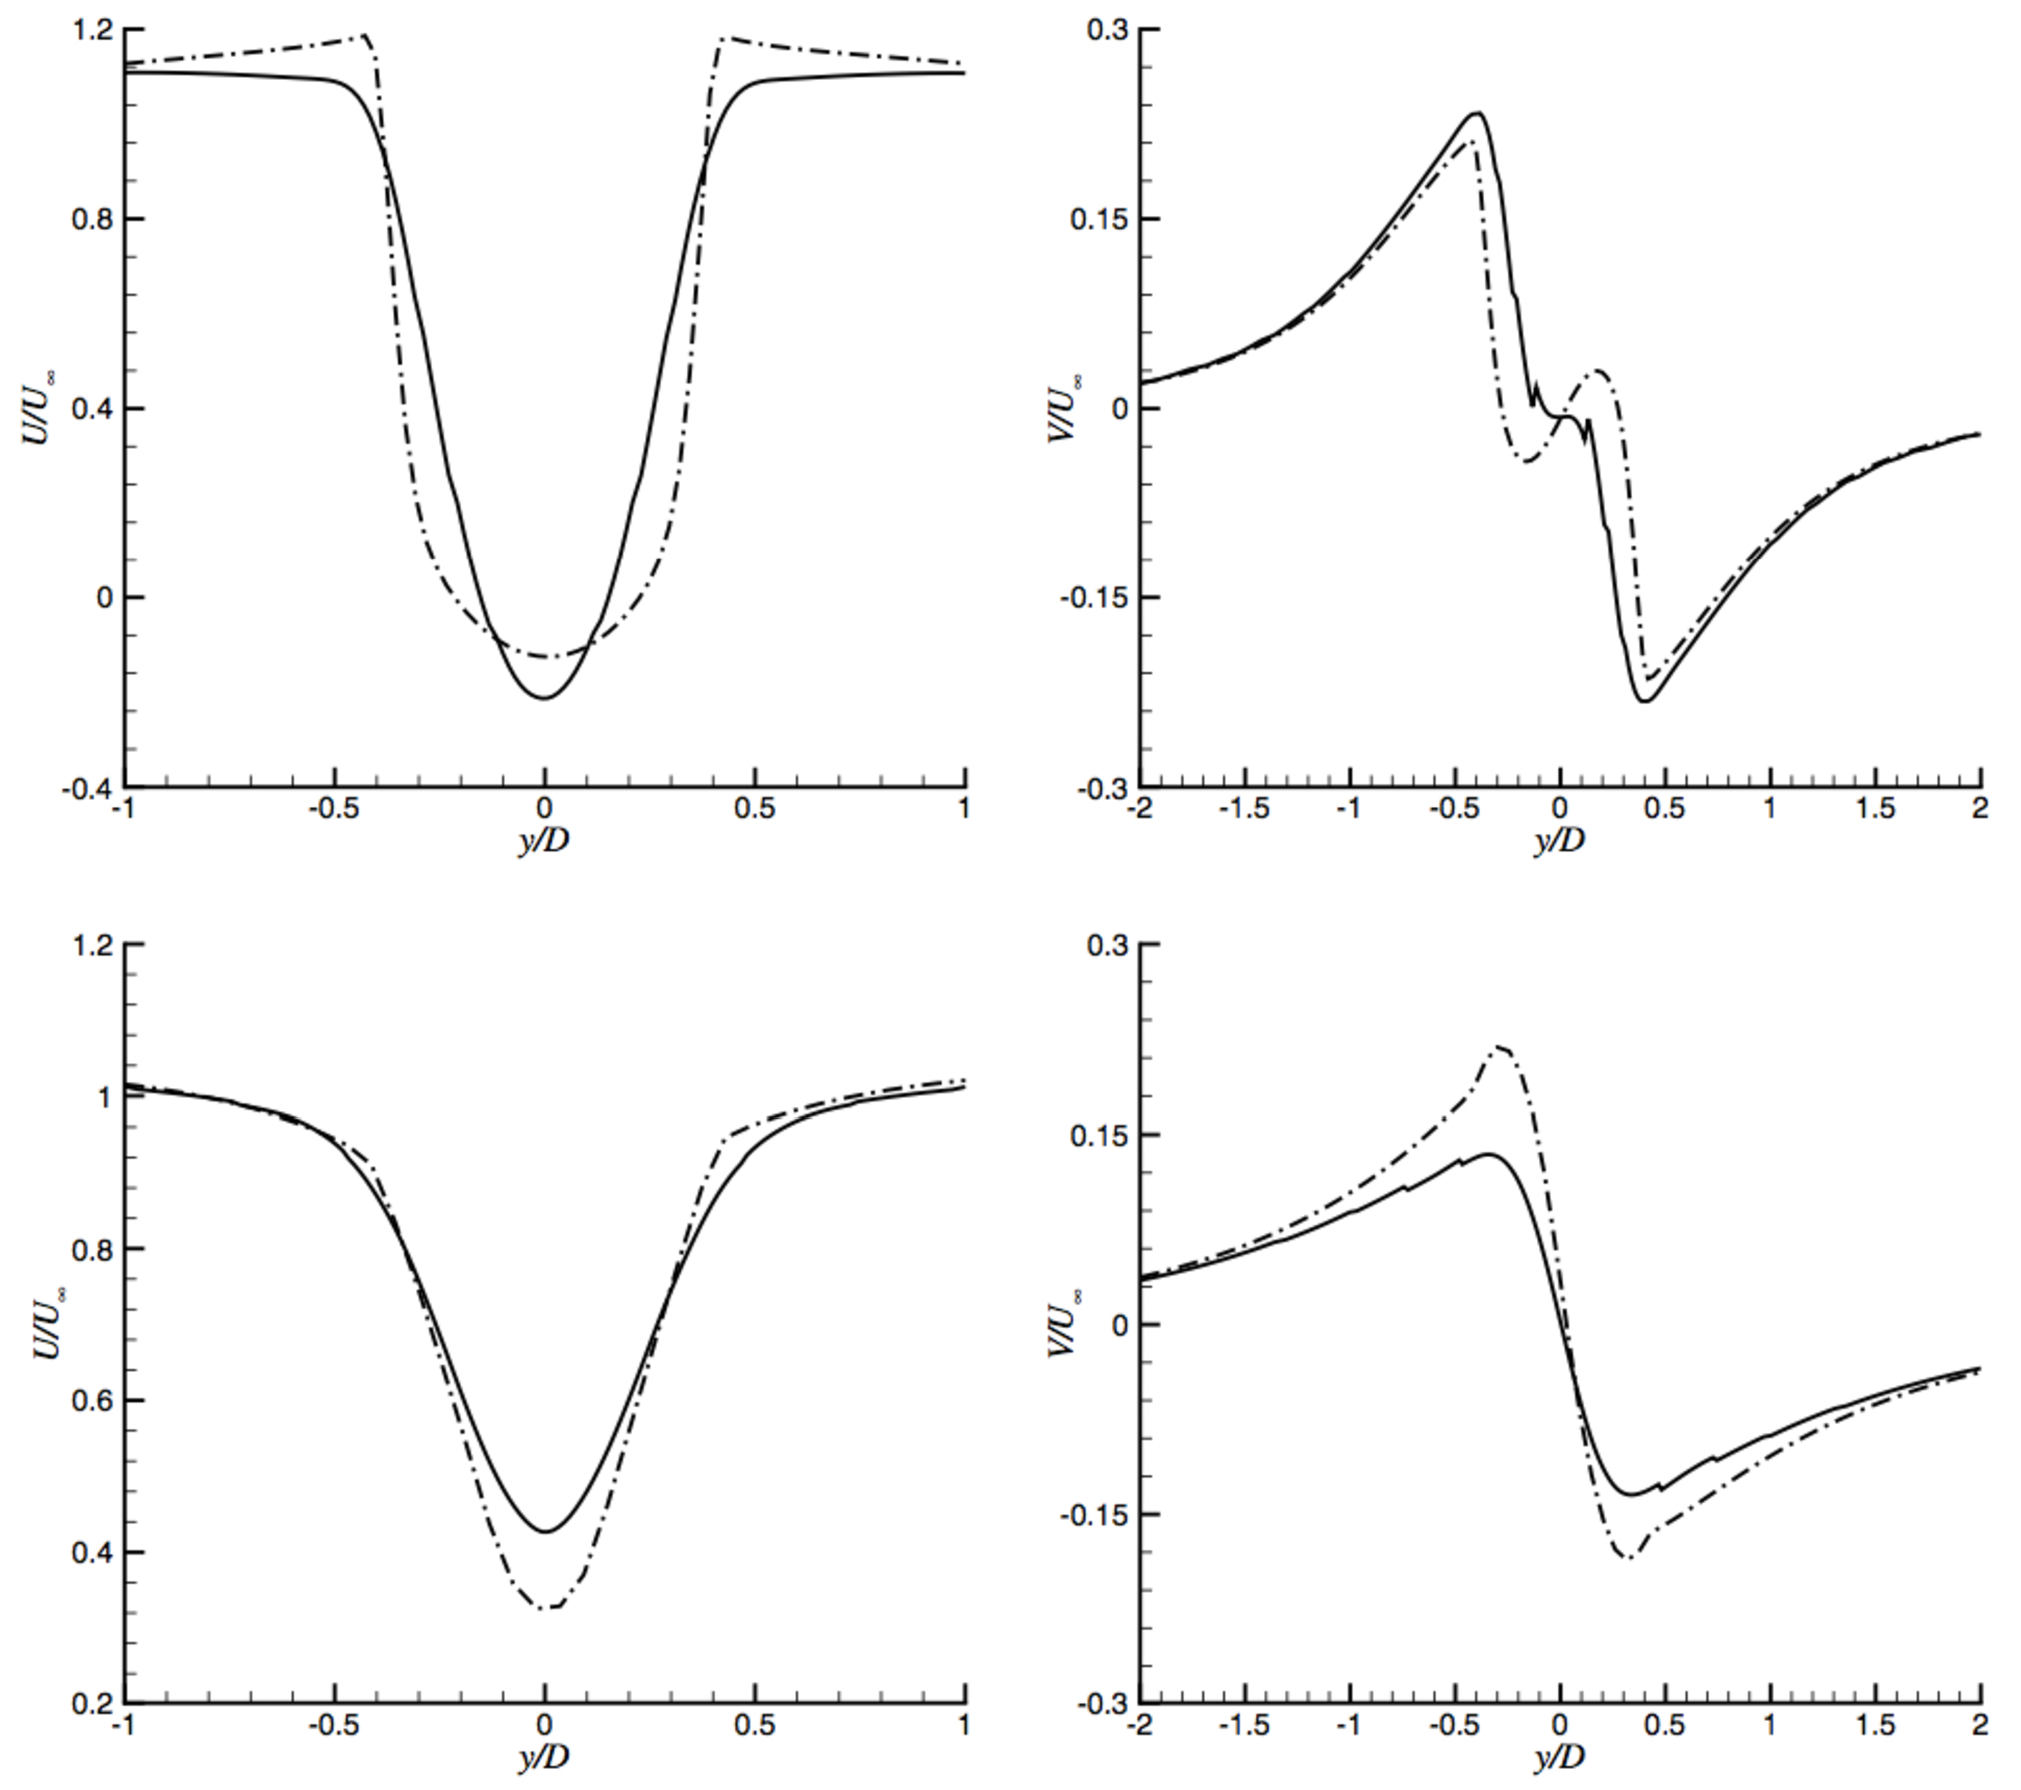
\includegraphics[width=0.5\textwidth]{Images/logan/catalano_2003numerical_VelocityProfiles.pdf}
% \caption{ cylinder les vs urans velocity profiles \cite{catalano2003numerical} }
% \label{fig:lesvsuranscylindervelprofile}
% \end{center}
% \end{figure}
% %%\vspace{-2em}

% Fig. 6. Mean streamwise and vertical velocities at x=D 1⁄4 0:75 (upper figures) and x=D 1⁄4 1:50 (lower figures): (—) LES; (– –) URANS



% %%%%%%%%%%%%%%%%%%%%%%%%%%%%%%%%%%%%%%%%%%%%%%%%%%%%%%%%%%%%

% %%% LES VS RANS CYLINDER GRID
% %%\vspace{-2em}
% % \begin{figure}[htb]
% \begin{figure}[H]
% \begin{center}
% 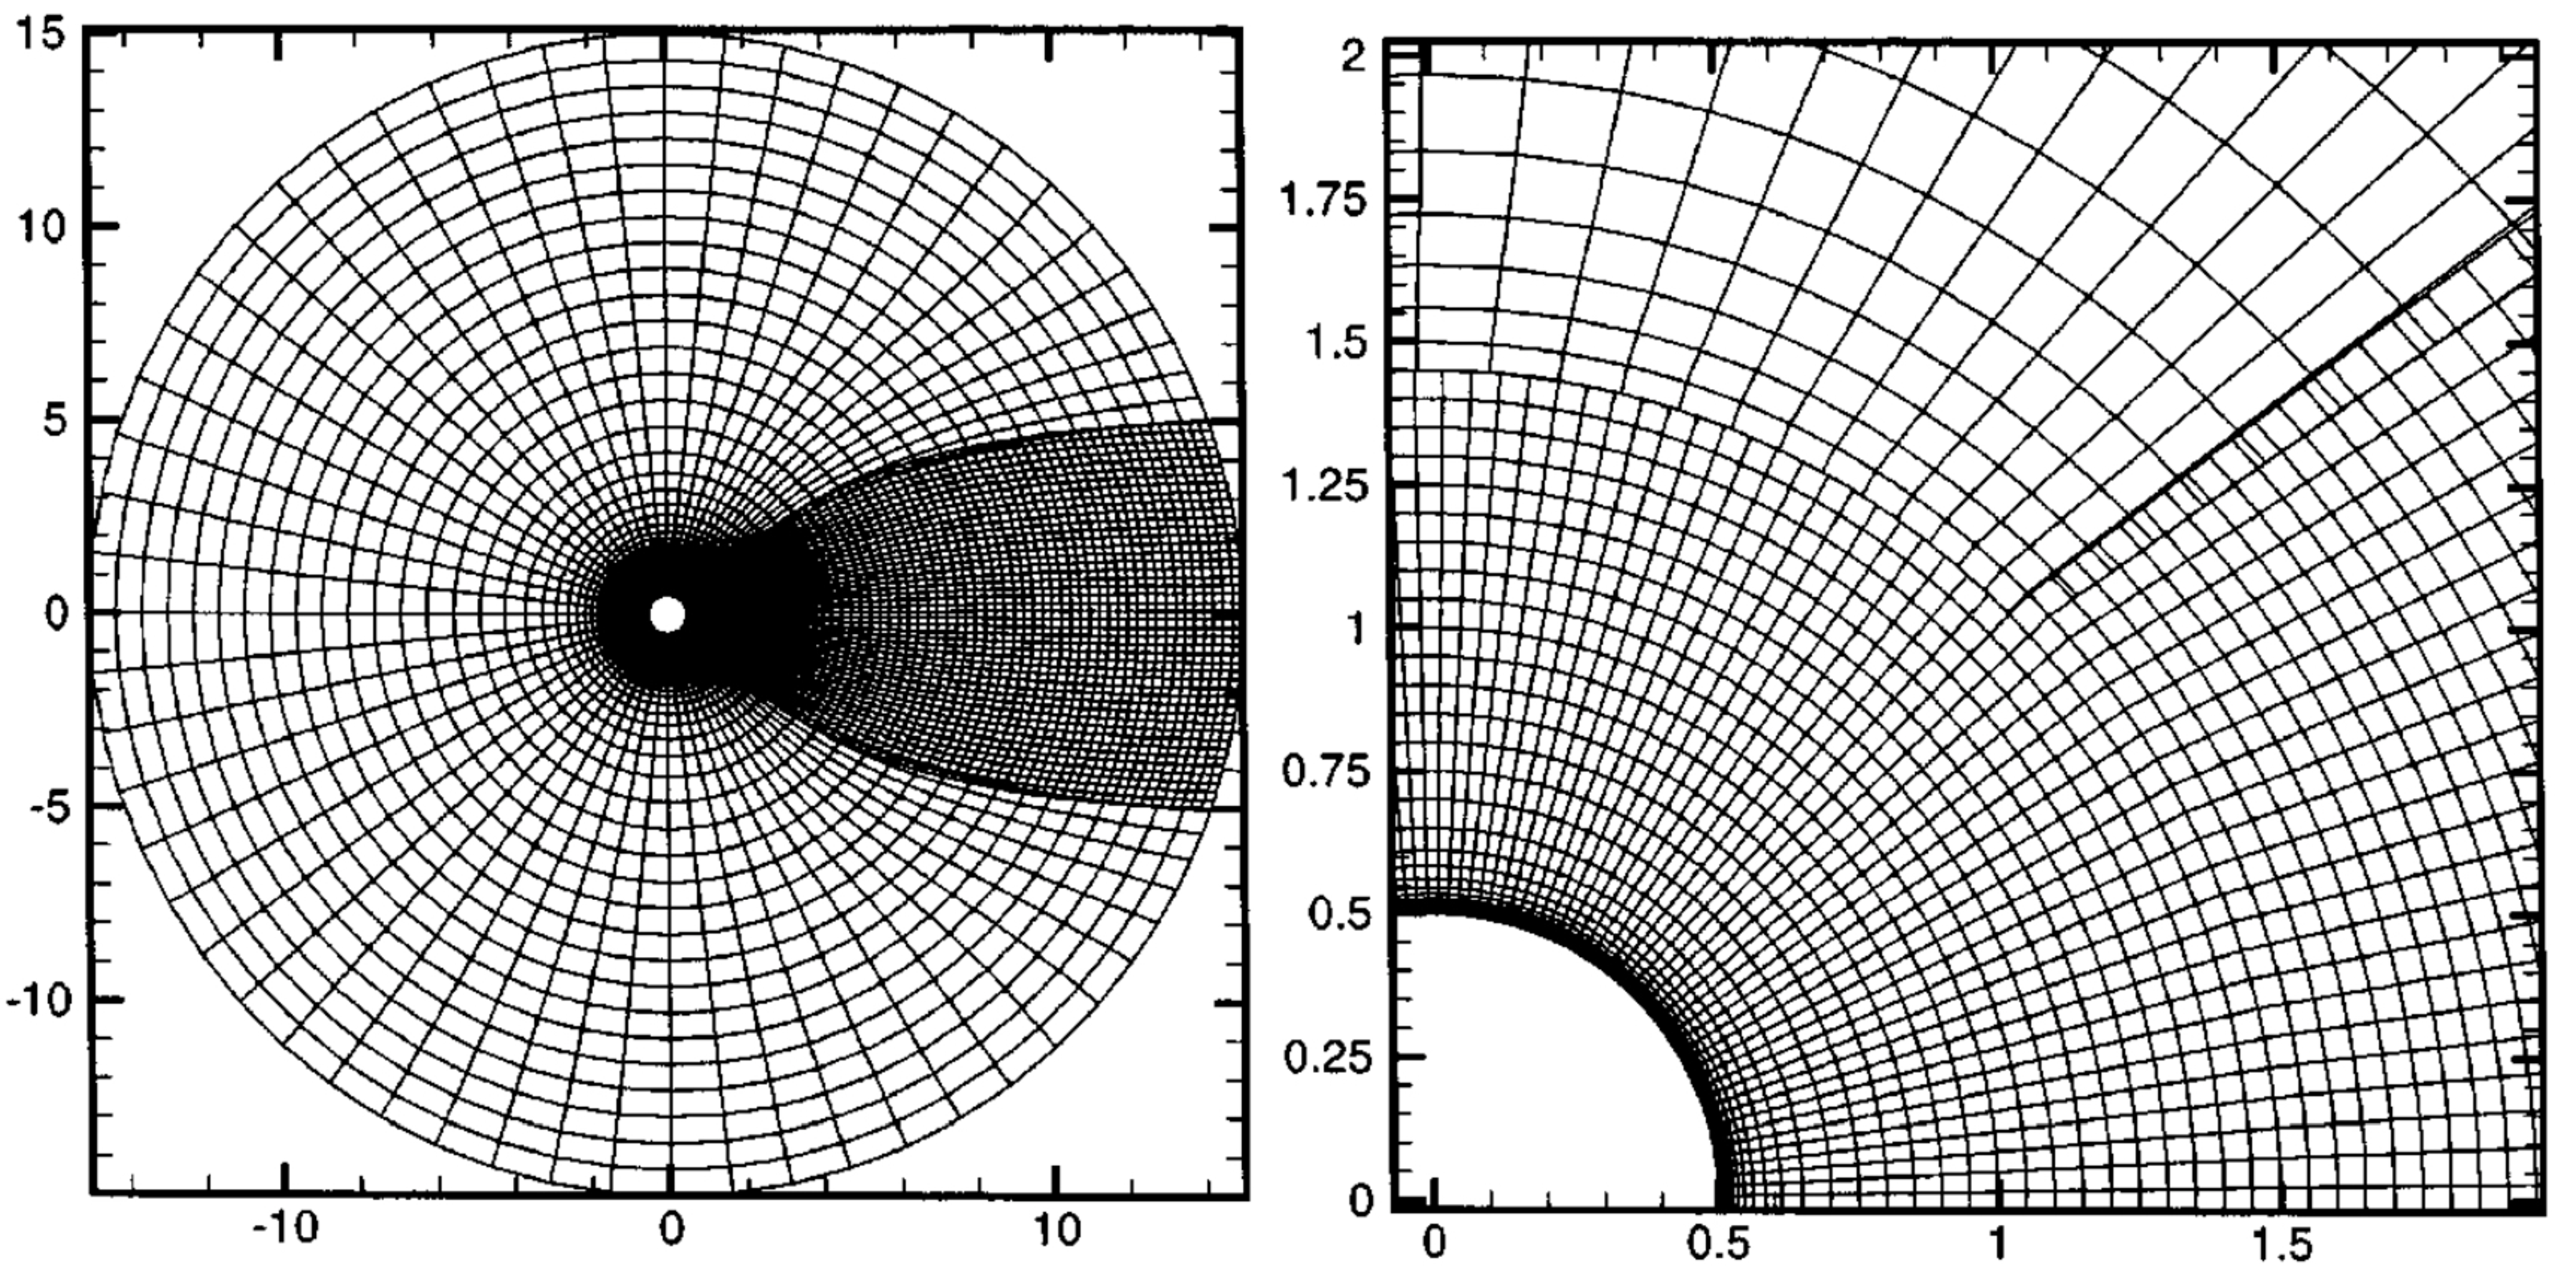
\includegraphics[width=0.5\textwidth]{Images/logan/travin2000detachededdy_grid.pdf}
% \caption{ cylinder les vs rans grid \cite{travin2000detachededdy} }
% \label{fig:lesvsranscylindergrid}
% \end{center}
% \end{figure}
% %%\vspace{-2em}

% Figure1. Medium computational grid, CaseTS2.Innerblock150×36,wakeblock74×36, outer block 59 × 30. The three blocks meet near x = 1.06, y = 1.03.  Grid for spalart cylinders.


% %%% LES VS RANS CYLINDER
% %%\vspace{-2em}
% % \begin{figure}[htb]
% \begin{figure}[H]
% \begin{center}
% 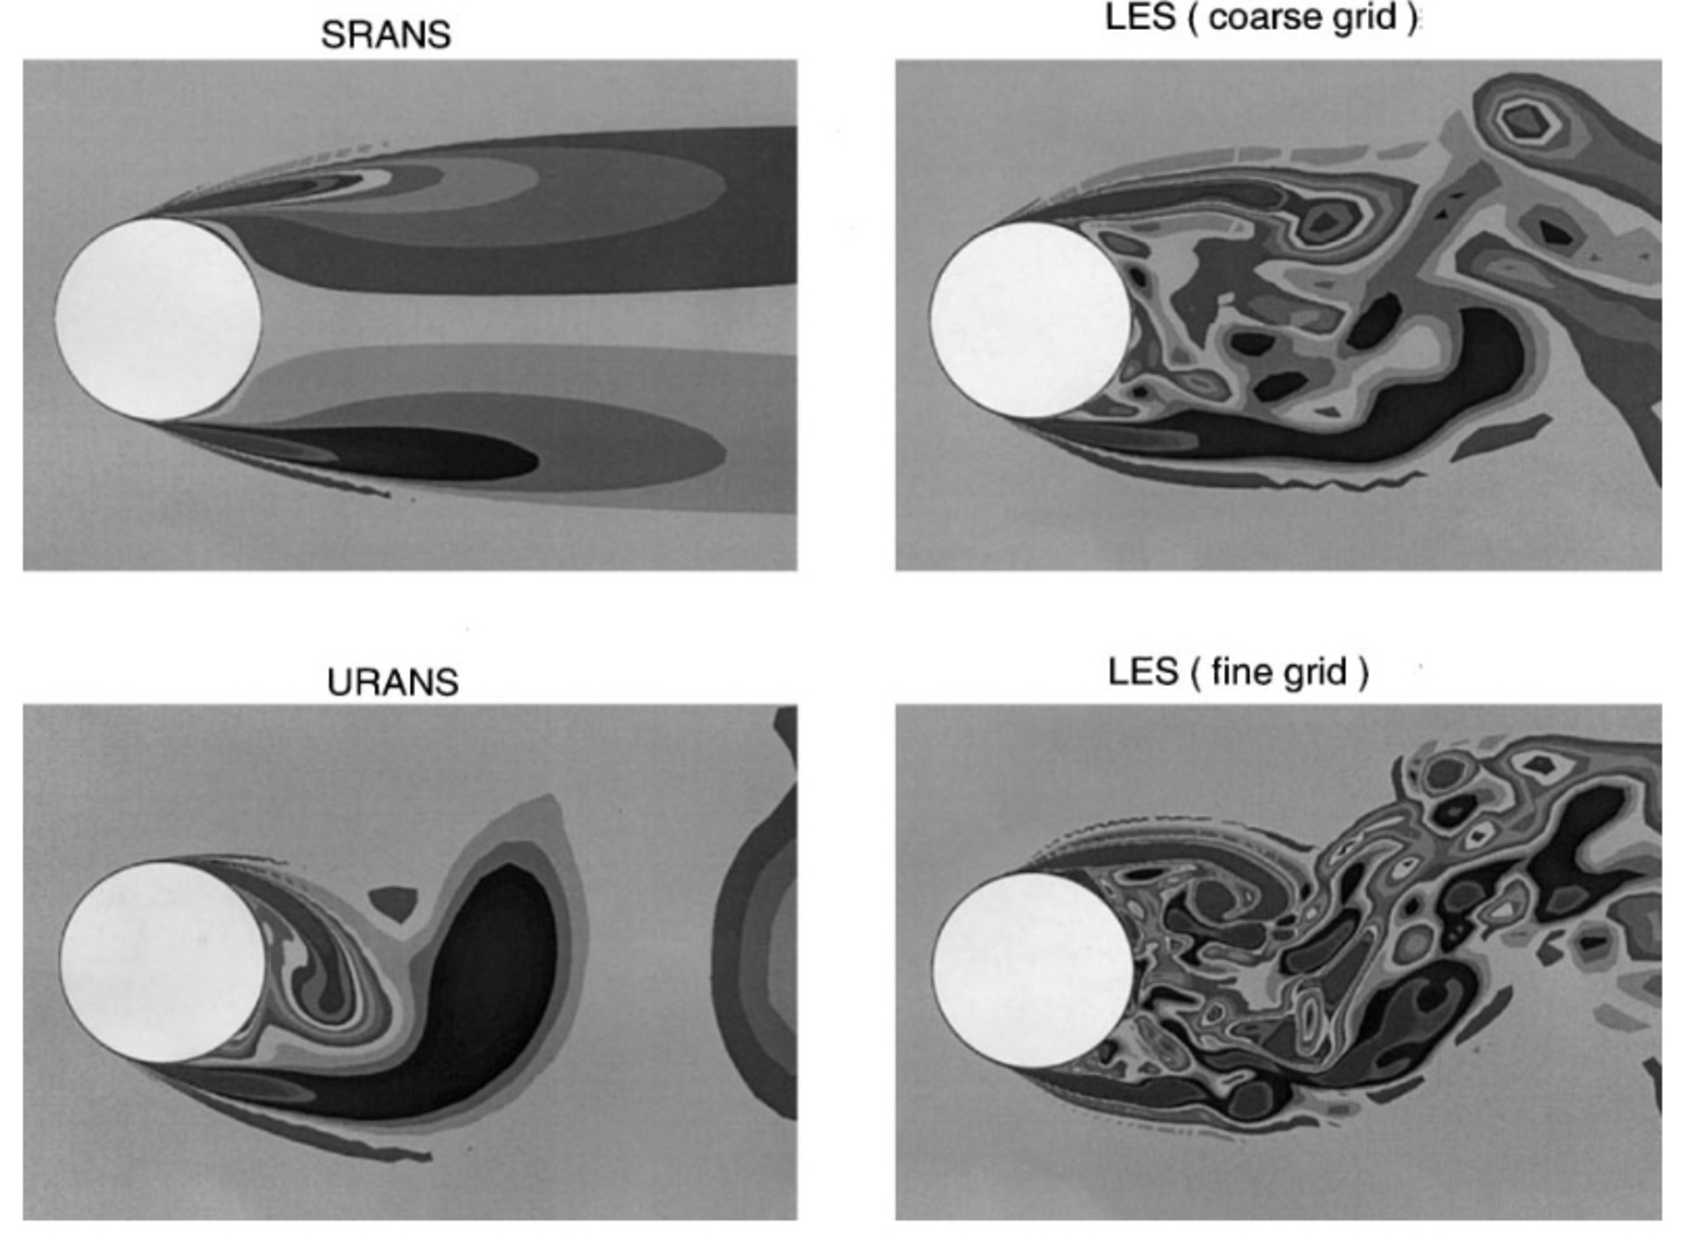
\includegraphics[width=0.5\textwidth]{Images/logan/spalart2000strategies_CylinderLESvsRANS.pdf}
% \caption{ cylinder les vs rans \cite{spalart2000strategies} }
% \label{fig:lesvsranscylinder}
% \end{center}
% \end{figure}
% %%\vspace{-2em}


% grid for LES shown above (actual simulations were DES)






%%%%%%%%%%%%%%%%%%%%%%%%%%%%%%%%%%%%%%%%%%%%%%%%%%%%%%%%%%%%


% %%% CURVE BACKSTEP VELOCITY PROFILE LES VS RANS
% %%\vspace{-2em}
% % \begin{figure}[htb]
% \begin{figure}[H]
% \begin{center}
% 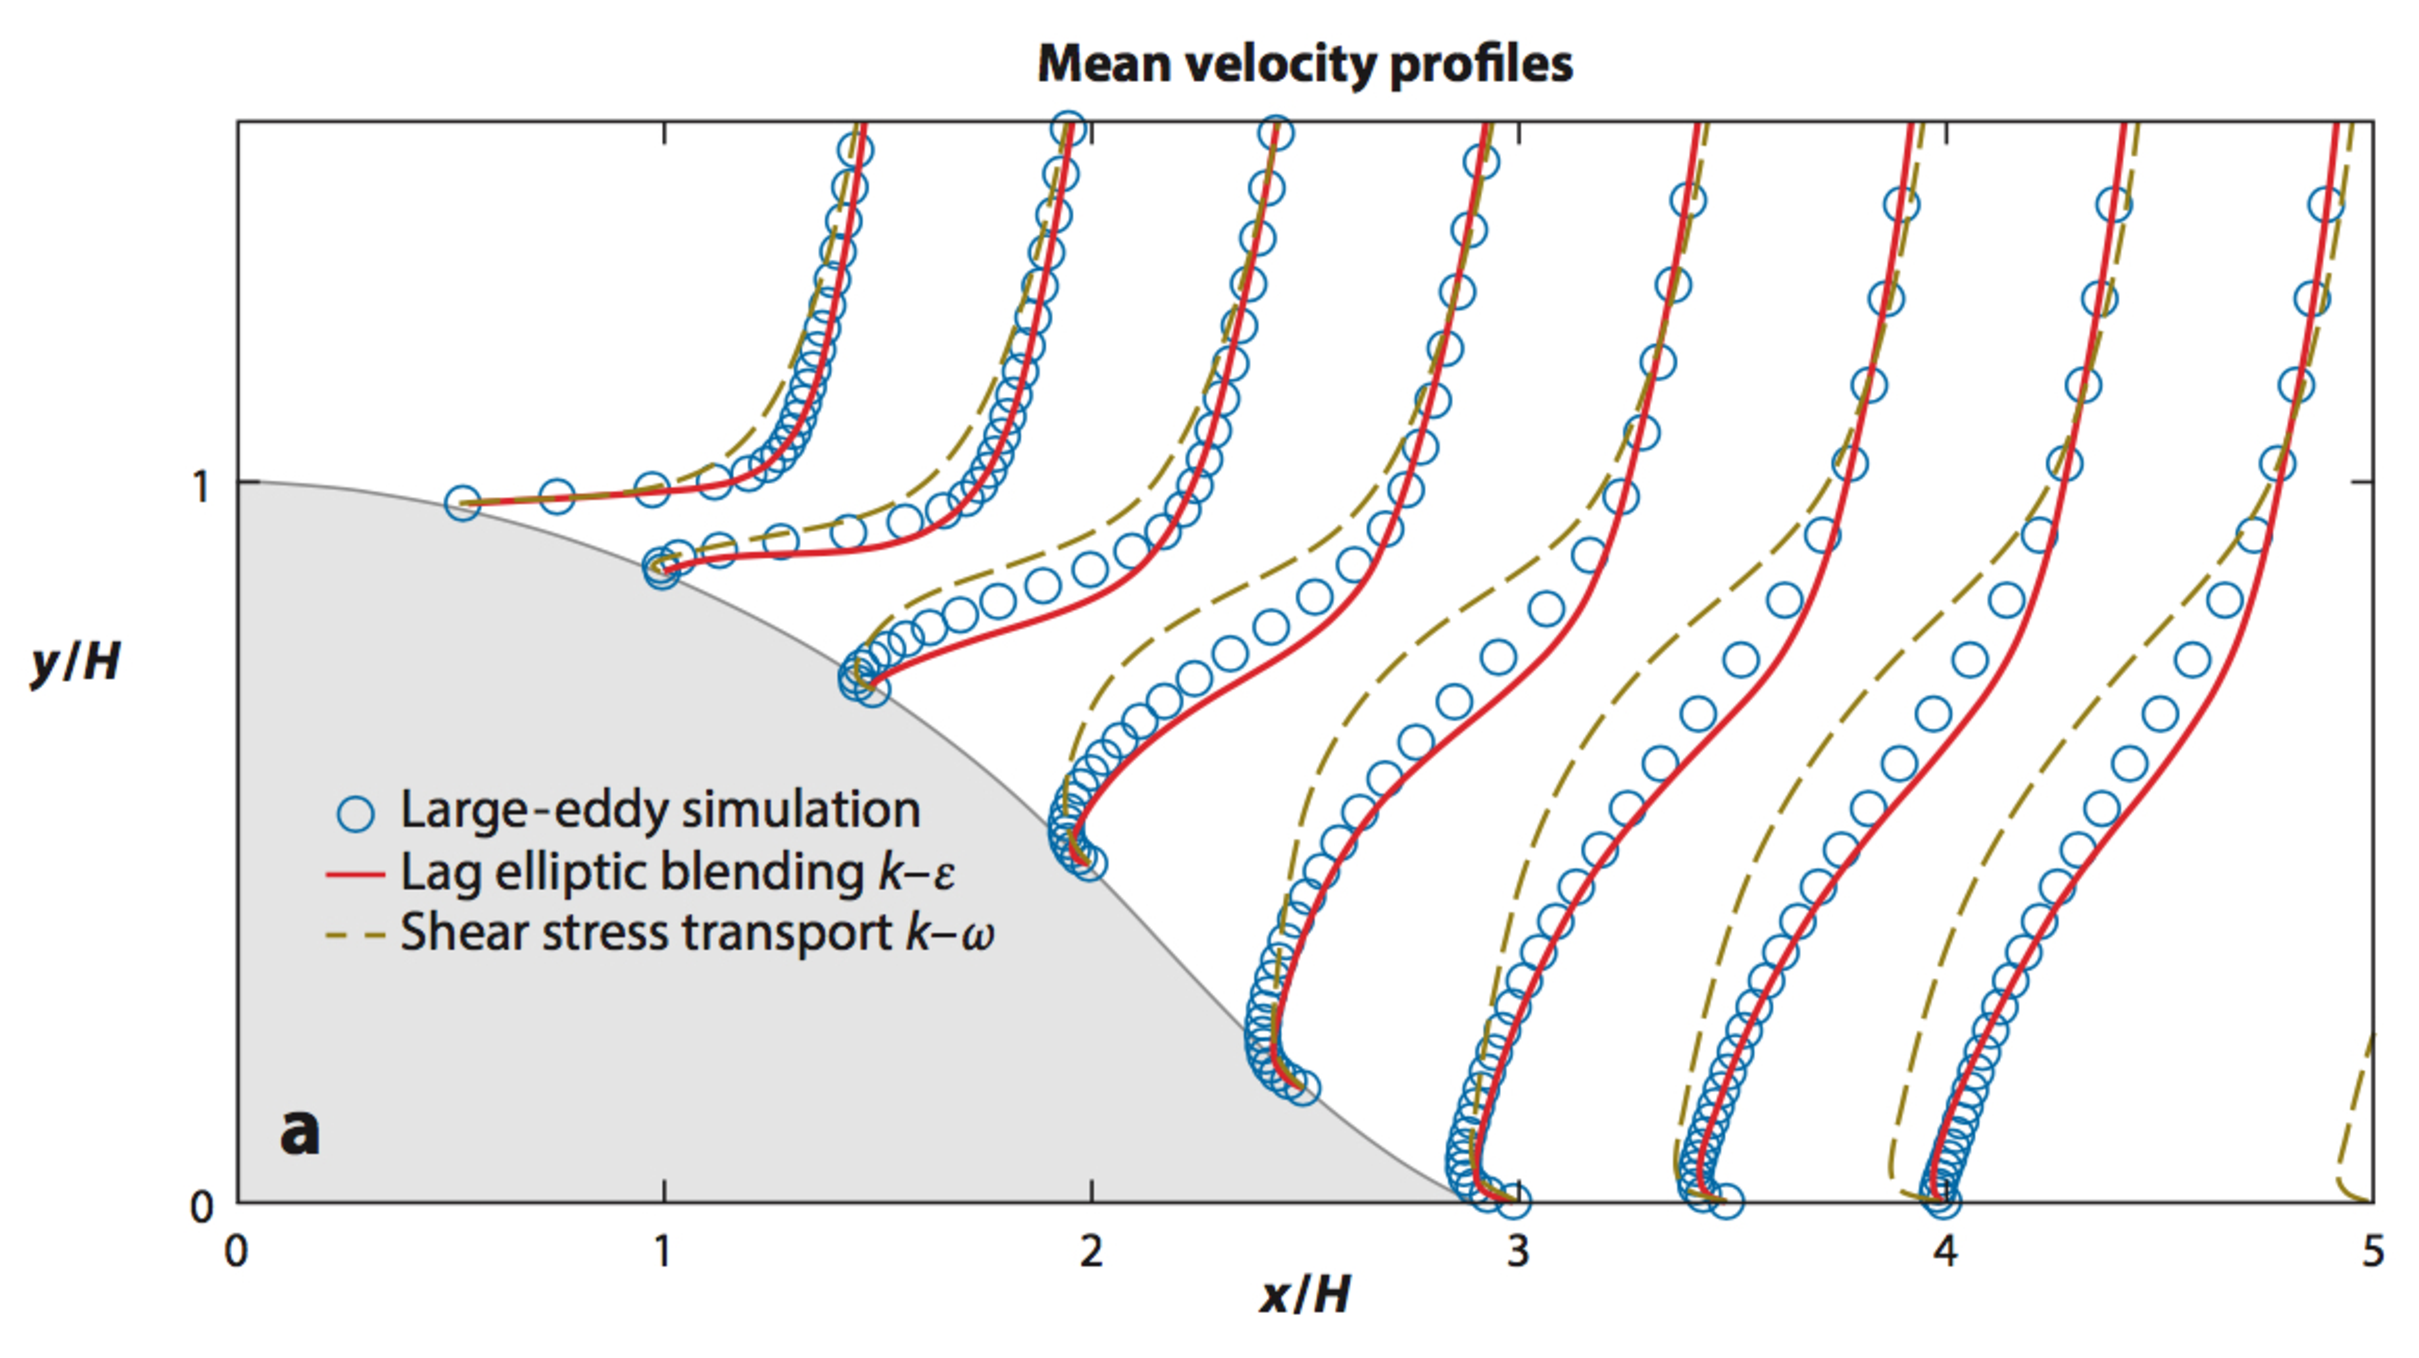
\includegraphics[width=0.5\textwidth]{Images/logan/durbin2018some_BackstepLESvsRANS.pdf}
% \caption{curve backstep velocity profile les vs rans \cite{durbin2018some}}
% \label{fig:lesvsransbackstep}
% \end{center}
% \end{figure}
% %%\vspace{-2em}










% %%% RECTANCULAR CYLINDER DNS
% %%\vspace{-2em}
% % \begin{figure}[htb]
% \begin{figure}[H]
% \begin{center}
% 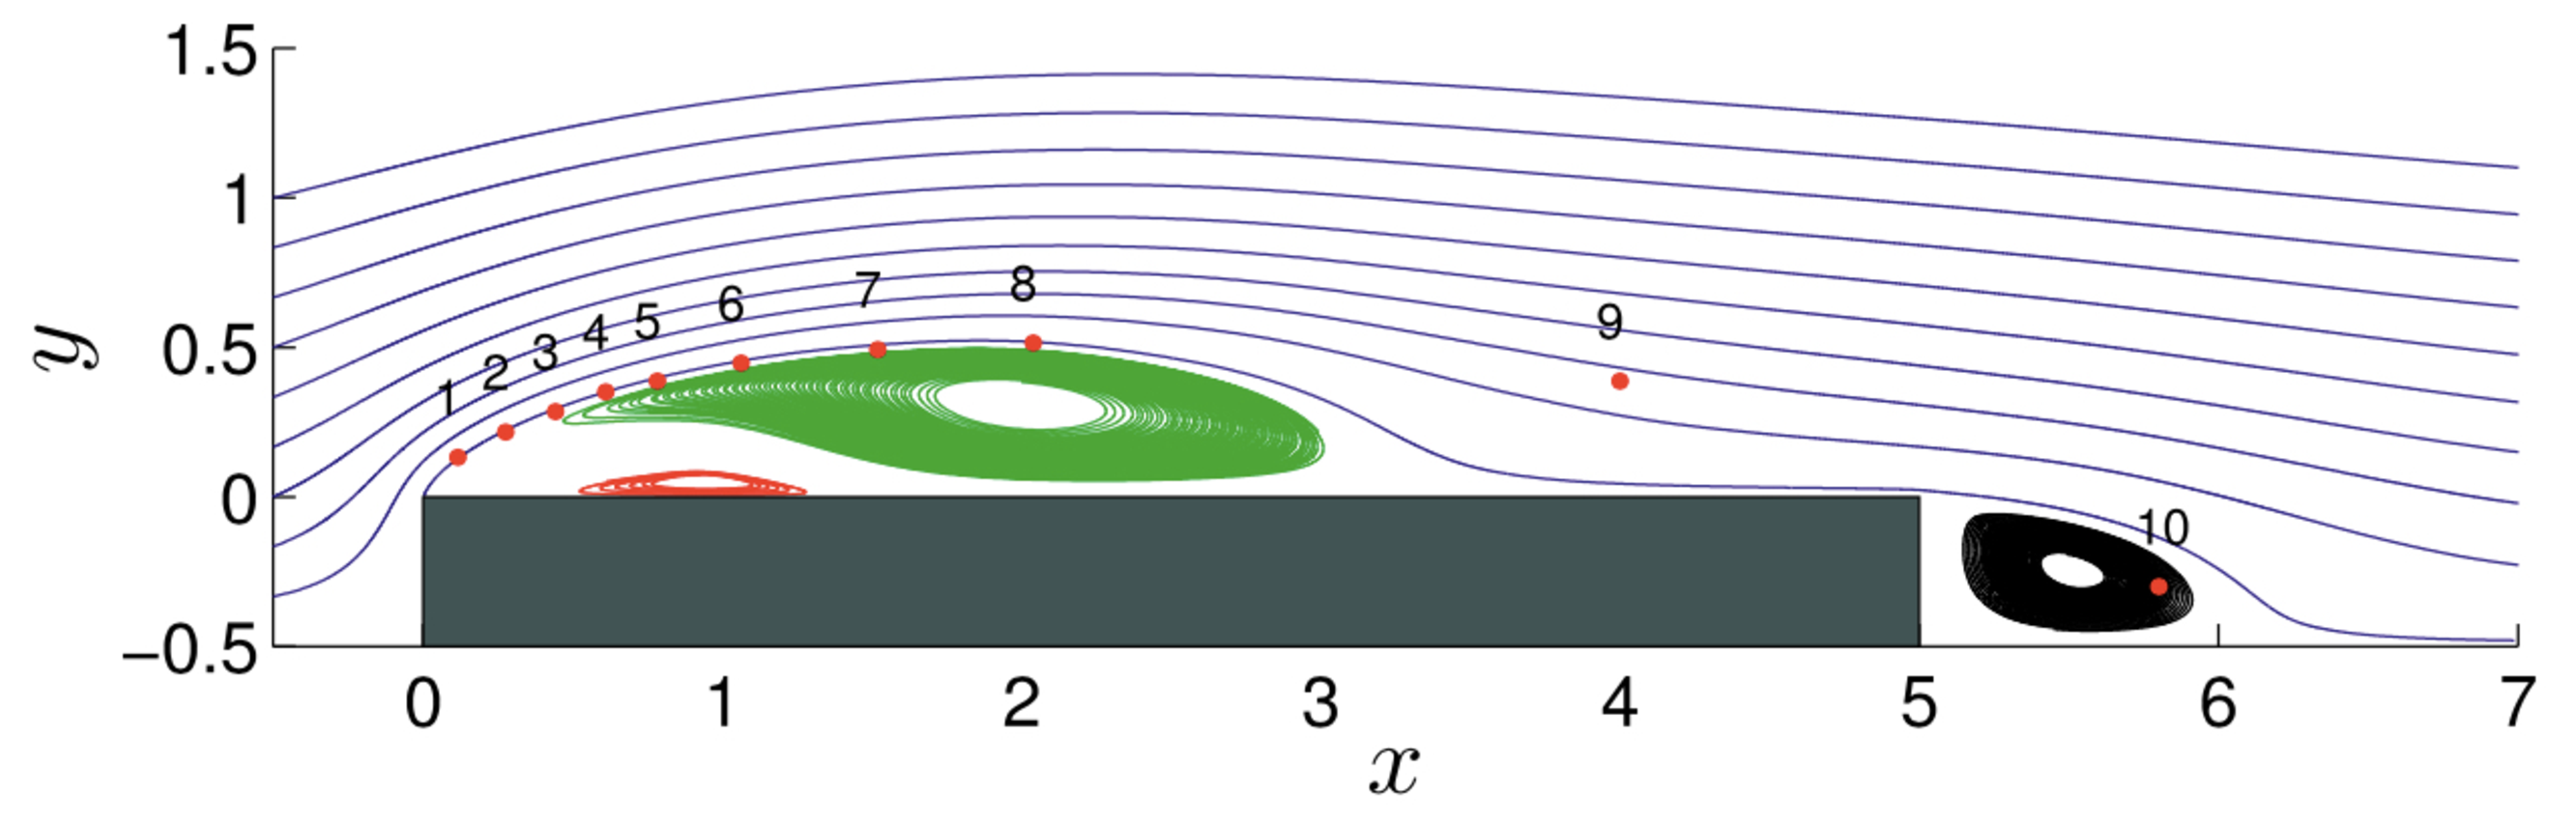
\includegraphics[width=0.45\textwidth]{Images/logan/cimarelli2018direct_vortices.pdf}
% \caption{ DNS square cylinder vortex locations Re=3000 \cite{cimarelli2018direct} }
% \label{fig:dnsRectCylVortices}
% \end{center}
% \end{figure}
% %%\vspace{-2em}


% Fig. 4. Streamlines of the mean velocity field (U,V) (x,y)  The green lines show the primary vortex, the red lines mark the secondary vortex and the black lines denote the wake vortex. The red dots denote the locations of the probes used for the computation of time spectra in section x5. (For interpretation of the references to color in this figure legend, the reader is referred to the Web version of this article.)

% %%\vspace{-2em}
% % \begin{figure}[htb]
% \begin{figure}[H]
% \begin{center}
% 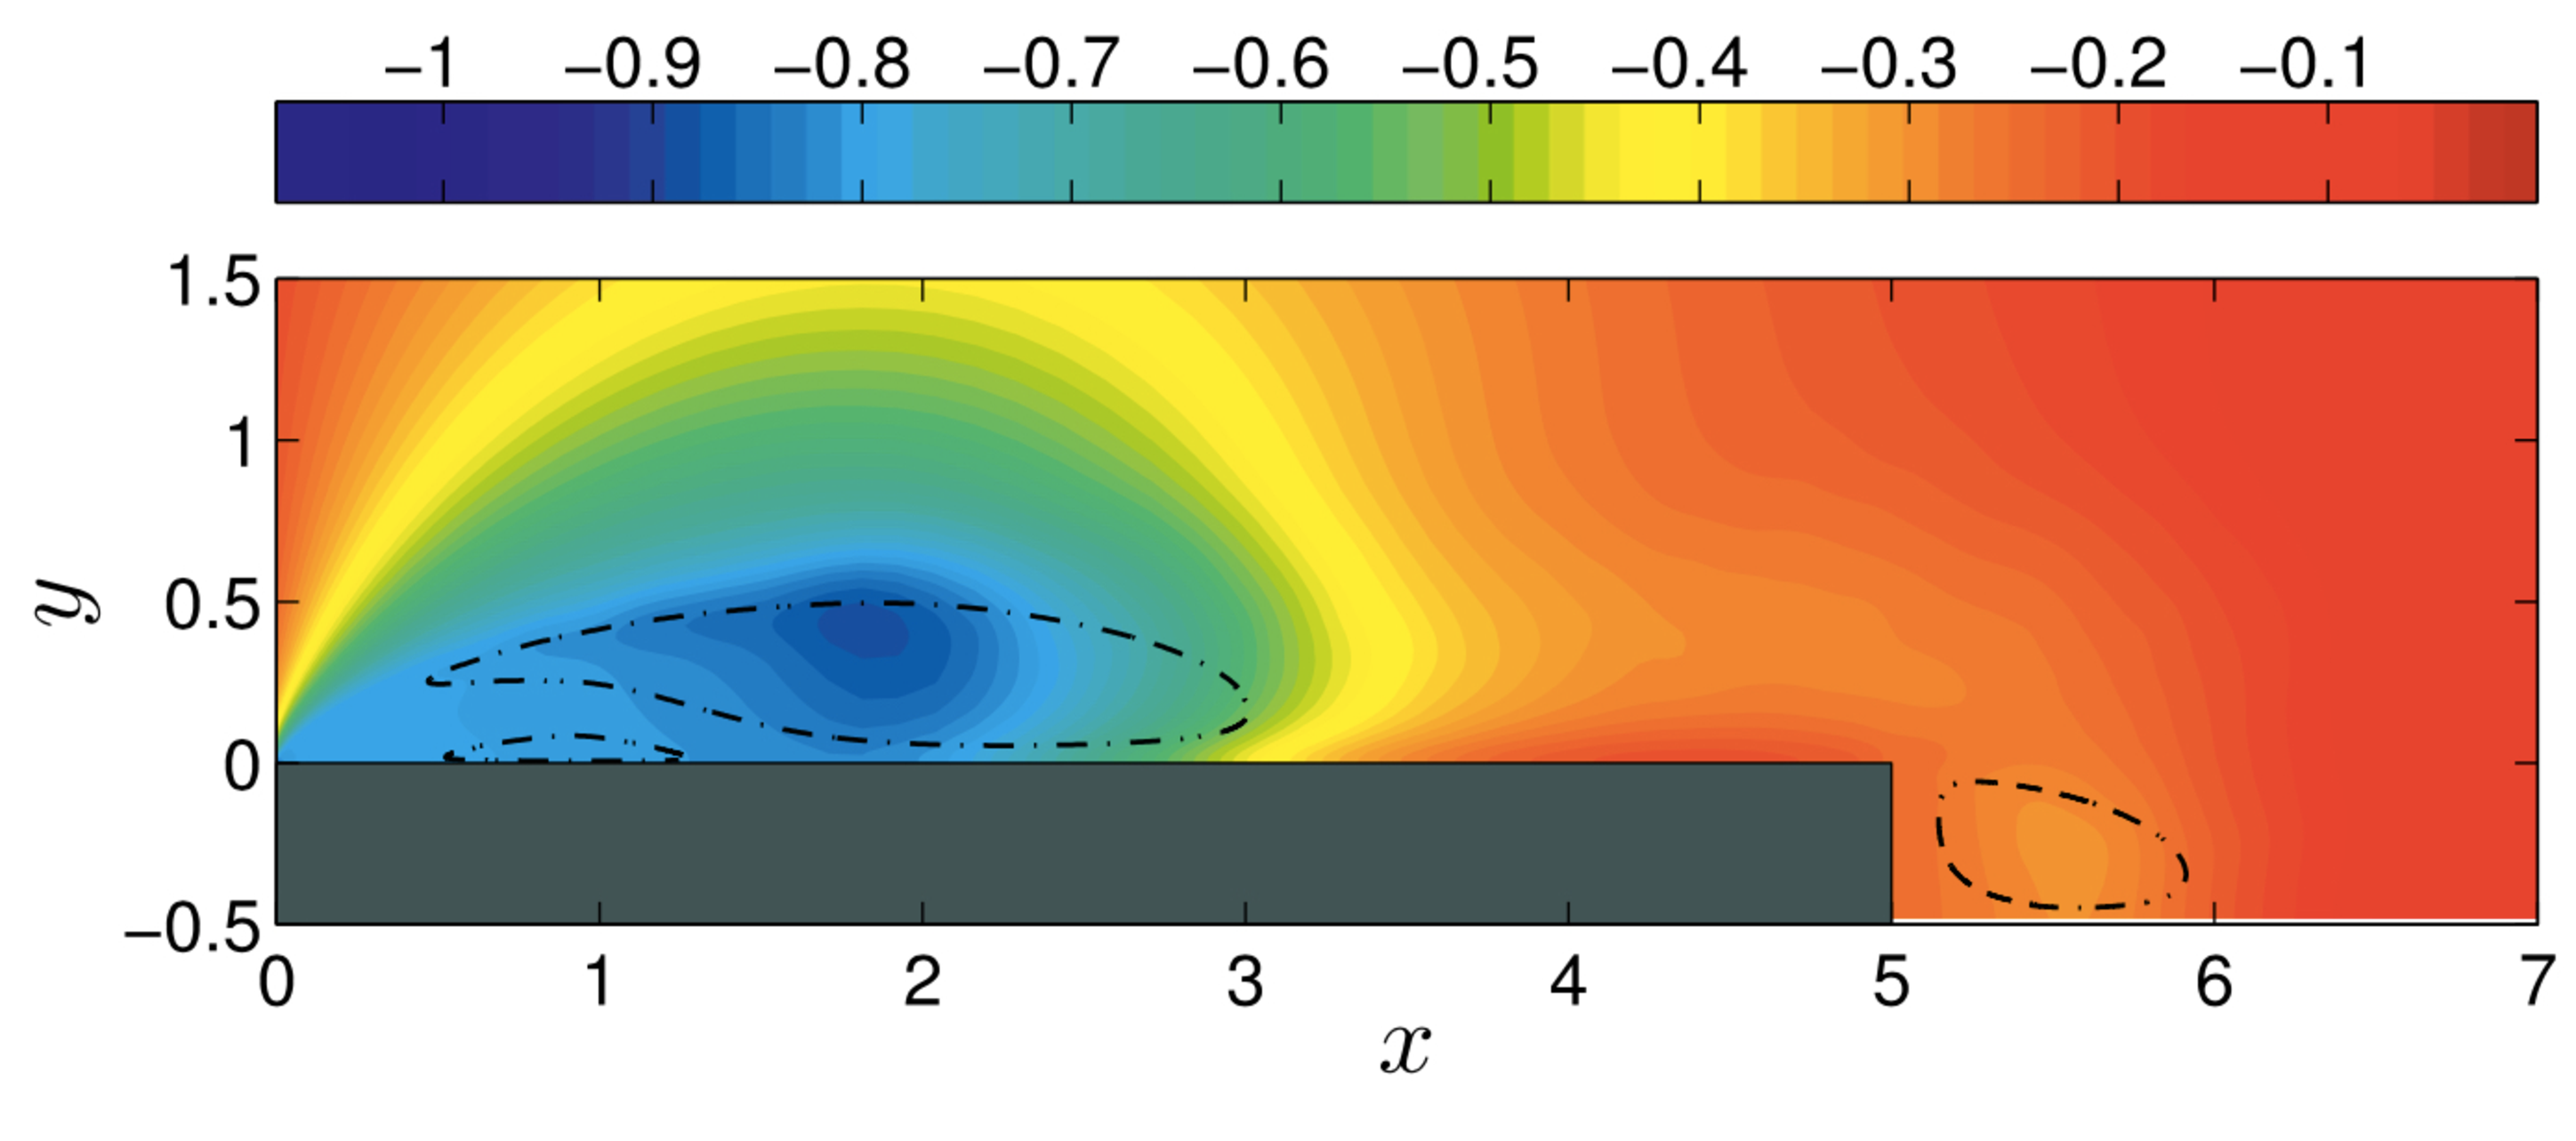
\includegraphics[width=0.45\textwidth]{Images/logan/cimarelli2018direct_pressure.pdf}
% \caption{ DNS square cylinder mean pressure distribution Re=3000 \cite{cimarelli2018direct} }
% \label{fig:dnsRectCylPressure}
% \end{center}
% \end{figure}
% %%\vspace{-2em}

% Fig. 5. Isocontours of the mean pressure field P(x,y). The dashed lines report the location of the primary vortex, secondary vortex and wake vortex.







% % DNS SQUARE CYLINDER FLOW
% %%\vspace{-2em}
% % \begin{figure}[htb]
% \begin{figure}[H]
% \begin{center}
% 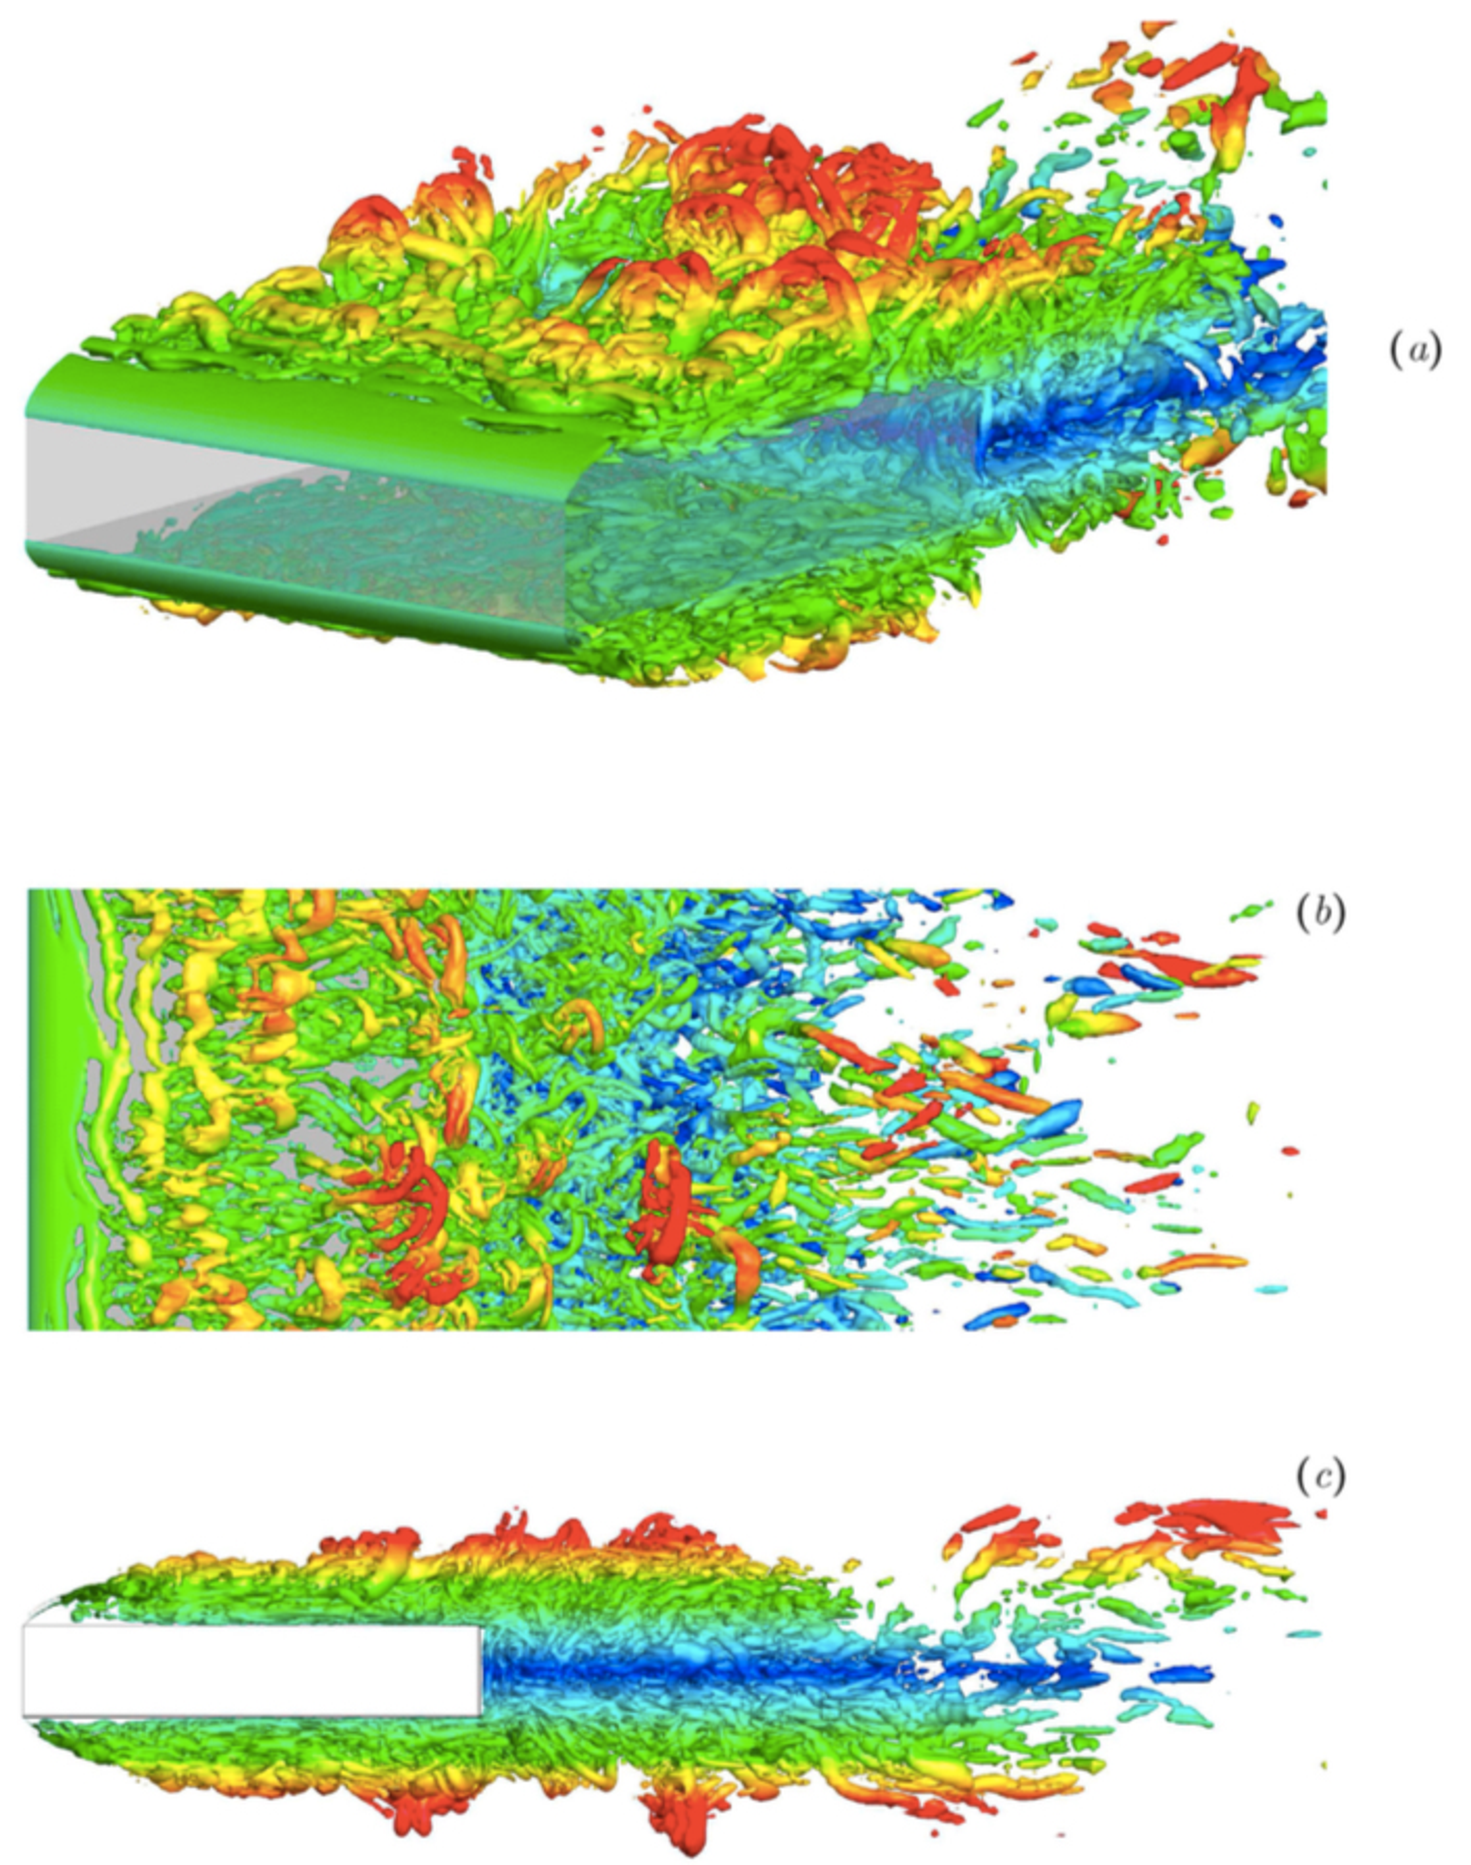
\includegraphics[width=0.5\textwidth]{Images/logan/cimarelli2018direct_vorticity.pdf}
% \caption{ DNS square cylinder vorticity contours Re=3000 \cite{cimarelli2018direct} }
% \label{fig:dnsRectCylPressure}
% \end{center}
% \end{figure}
% %%\vspace{-2em}

% Fig. 10. Instantaneous isosurfaces of $\lambda_2=-2$ colored with $y$. Perspective, top and lateral views in (a), (b) and (c) plots, respectively.










%%%%%%%%%%%%%%%%%%%%%%%%%%%%%%%%%%%%%%%%%%%%%%%%%%%%%%%%%%%%%%%%%%%%%%%%
\section{Conclusions}
%%%%%%%%%%%%%%%%%%%%%%%%%%%%%%%%%%%%%%%%%%%%%%%%%%%%%%%%%%%%%%%%%%%%%%%%

Bluff-body flow accounts for an innumerable amount of real-world applications, ranging from high-angle-of-attack fighter aircraft to buildings in a hurricane. Furthermore, flow over simple bluff-bodies like cylinders and spheres serve as common test cases for solver and experiment calibration. The complex nature of the massively separated wake behind a bluff body and the spectra of turbulence that develops within this flow region makes deciphering bluff-body flow through experiment and modeling both a difficult challenge and an essential task for understanding unsteady loading, stability characteristics, acoustics, and a number of other flow effects.

\textcolor{red}{\emph{FZ: Experimental methods summary/current state}}

This review has made the case for a combination of URANS and DES as the current state-of-the-art in bluff-body wake modeling. Pure DNS currently demands to much computational power for realistic bluff-body applications. URANS is cost-effective and suitable for obtaining time-averaged results for certain bluff-body geometries and conditions, but will prove insubstantial in some situations. DES provides higher-fidelity simulation of bluff-body turbulence but comes with its own set of guidelines and pitfalls. In short, simulations must still be designed with a deep understanding of the flow physics and methodology limitations to obtain reasonable results, but when this knowledge is applied and simulations are validated according to experimental examples, accurate representations of bluff-body flow for a wide range of conditions can be obtained numerically. In the future, advances in computational power and intelligent solver algorithms will continue to improve the usability and accuracy of CFD applied to bluff-body geometries.






% %%%%%%%%%%%%%%%%%%%%%%%%%%%%%%%%%%%%%%%%%%%%%%%%%%%%%%%%%%%%%%%%%%%%%%%%
% \section*{Acknowledgments} %%%%%%%%%%%%%%%%%%%%%%%%%%%%%%%%%%%%%%%%%%%%%
% %%%%%%%%%%%%%%%%%%%%%%%%%%%%%%%%%%%%%%%%%%%%%%%%%%%%%%%%%%%%%%%%%%%%%%%%

% \textcolor{red}{\emph{LH\&FZ}}

%%%%%%%%%%%%%%%%%%%%%%%%%%%%%%%%%%%%%%%%%%%%%%%%%%%%%%%%%%%%%%%%%%%%%%%%
%%% BIBLIOGRAPHY %%%%%%%%%%%%%%%%%%%%%%%%%%%%%%%%%%%%%%%%%%%%%%%%%%%%%%%
%%%%%%%%%%%%%%%%%%%%%%%%%%%%%%%%%%%%%%%%%%%%%%%%%%%%%%%%%%%%%%%%%%%%%%%%


%bibliography from .bib file, filename goes in {}
%NOTE: References must be cited with "\cite" command to appear in bibliography
%Types of Refs: article, book, conference=inproceedings, manual, mastersthesis, phdthesis, techreport, unpublished, misc (see "new-aiaa.bst")
%when you first initialize .bib file, might need to have plain text in front of \cite command to get sublime text to recognize bibliography file
\bibliography{BluffBodyTurb}

\end{document}
